\documentclass[12pt]{report}
\usepackage{graphicx}
\usepackage{hyperref}
\usepackage{fancyhdr}
\usepackage{graphicx}
\usepackage{caption}
\usepackage{subcaption}
\usepackage{amssymb,amsmath}
\usepackage[]{algorithm2e}
\usepackage{listings}
\usepackage{dashrule}
\usepackage{tikz}
\usepackage{forest}
\usepackage{nameref}
\usepackage{amsthm}
\theoremstyle{definition}
\newtheorem{definition}{Definition}[section]
\graphicspath{ {images/} }
\usepackage{array}
\newcolumntype{L}[1]{>{\raggedright\let\newline\\\arraybackslash\hspace{0pt}}m{#1}}




\newcommand{\myrule} [3] []{
    \begin{center}
        \begin{tikzpicture}
            \draw[#2-#3, ultra thick, #1] (0,0) to (1.0\linewidth,0);
        \end{tikzpicture}
    \end{center}
}

\pagestyle{fancy}
\fancyhead[LE,RO]{\itshape \nouppercase \rightmark}
\fancyhead[LO,RE]{\itshape \nouppercase Chapter \arabic{chapter}}

\begin{document}
\begin{titlepage}
  \begin{flushleft}
   
\includegraphics[width=0.5\textwidth]{tulogo.png}\par\vspace{1cm}
  \end{flushleft}
  \centering
	\myrule{}{}
	{\huge\bfseries Elastic Load Scaling for Audio/Video Conferencing Services\par}
	\myrule[double]{}{}
	\vspace{2cm}
	{\scshape\Large Subramanya Umashankar Joshi\par}
	\vspace{1.5cm}
  \begin{flushleft}
  {\textit{Professor:}\hspace{0.7cm}Prof. Dr. rer. nat. habil. Dr. h. c. Alexander Schill\par}
	{\textit{Supervisor:}\hspace{0.5cm}M.Sc. Kateryna Rybina\par}
  \end{flushleft}
	\vspace{1.5cm}
  \centering
  {Master thesis submitted in fulfilment of the requirements for the degree of M.Sc. Distributed Systems Engineering in the Chair of Computer Networks, Faculty of Computer Science.\par}
  \vspace{0.2cm}
	{\large \today\par}
\end{titlepage}

\bibliographystyle{abbrv}

\chapter*{}
\thispagestyle{empty}

\chapter*{Abstract}

Recently cloud computing is know to change the way applications are designed and deployed. Cloud systems use virtualization technologies (such as Xen, KVM etc.) to allocate on-demand IT resources in terms of virtual machines (VM). This on-demand allocation is called scaling. Scalability is a critical issue to the success of application involved in using cloud as hosting platform. Organizations which use cloud for hosting their application have Quality of Service (QoS) guaranties to fulfill in accordance with service level agreements with their customers. Automated scaling mechanisms hold the promise of assuring QoS properties to the applications while simultaneously making efficient use of resources and keeping operational cost low.
\\
\\
Despite the advantages of automated scaling, realizing the full potential of automated scaling is hard due to the challenge of precisely estimating the resource need when system has arbitrary workload. Along with arbitrary workload, Infrastructure-As-A-Service (IaaS) cloud providers (such as Amazon AWS) offer diverse virtual machine instance purchasing options, such as on-demand instances, reserved instances, and spot instances. Such diverse pricing models make it challenging to determine how to optimally provision the required number of VM instances in different types to satisfy arbitrary workload demands. Given the limited budget, service providers need to carefully balance the VM provisioning cost and achieve QoS for end users.
\\
\\
This thesis introduces a threshold based automated scaling algorithm, named AppElastic. AppElastic algorithm deals with the horizontal scalability in IaaS mode. It address the trade-off problem between cost and QoS guaranties by employing very popular threshold based rules to automate scaling. AppElastic employs time series forecasting to proactively provision VM needed to satisfy the QoS guaranties. Furthermore, to mitigate rapid starting and stopping of VM's due to arbitrary workload, AppElastic algorithm is developed to terminate the VM's which are nearing instance-hour. The developed system is a customer oriented solution that could be extended to any cloud application to achieve horizontal scalability.

\pagestyle{fancyplain}
\fancyhf{}

\chapter*{}
\thispagestyle{empty}

\chapter*{Declaration}
I, Subramanya Umashankar Joshi, hereby declare that this thesis is my original and independent work. It has never been published and/or submitted for any award of degree to any other institution. All source of information have been acknowledged by references.
\\
\\
\\
\\
\\
\\
\\
\\
\\
\\
\\
\hdashrule{4cm}{1pt}{1pt} \\
Subramanya Umashankar Joshi\\
Dresden, 09.06.2016

\thispagestyle{empty}

\chapter*{}
\tableofcontents
\thispagestyle{empty}

\pagestyle{fancy}
\fancyhead[LE,RO]{\itshape \nouppercase \rightmark}
\fancyhead[LO,RE]{\itshape \nouppercase Chapter \arabic{chapter}}
\fancyfoot[CE,CO]{\thepage}
\setcounter{page}{0}
\chapter{Introduction}
\label{chap:Introduction}


Cloud computing\cite{mell2011nist} is a technology that is becoming extensively popular and usually is referred to being massively scalable. This is primarily due to the fact of cloud computing's elastic nature. Elasticity in cloud is generally referred for the usage of cloud resources on-demand\cite{mell2011nist}, and pay only for the resources being used. The resources provisioning are usually in the form of virtual machines (VM). Provisioning of VM is made possible through distributed, large-scale computing clusters, often driven by server virtualization software, like VMware ESX Server\cite{vmwareesx}, Xen\cite{xenhyper} or KVM\cite{kvmhyper}. Organizations which use or migrate to cloud, use cloud for different purposes such as running batch jobs, hosting web application or for storage and backup.
\\
Cloud hosted applications are likely to deliver high quality of service (QoS). The workload of an hosted application varies according to the time of the day and rises sharply on certain trends. For example, an online retailer faces spikes of workload on a new launch of smartphone and a daily cyclical workload variations\cite{dawoud2013scalability}. On the other hand, a video on demand provider anticipate peak workload on a video going viral\cite{niu2012quality}. However, the cloud infrastructure provides an elastic environment for these applications to scale up and down according to workload variations.

\section{Motivation}
\label{sec:Motivation}
Cloud computing architecture enables an application to cope with rapidly varying workloads. Timely provisioning VM's in the cloud implies an overhead. The overhead can lead to period of over-utilization of the VM's which degrades the QoS. Moreover, due to workload consolidation in cloud infrastructures, the performance of an application can be influenced by other co-located VM's. Few of the several challenges faced while managing the performance of an application while maintaining high QoS are listed below:
\begin{itemize}
  \item \textbf{Resource Acquisition} The overhead of provisioning a right VM instance type and right number of VM instances in public or private cloud is a problem. The overhead is attributed to the IaaS cloud vendors, such as Amazon EC2\cite{amazon2010amazon}, Rackspace\cite{rackspace2010inc},etc., apply diverse VM instance pricing models at different commitment levels. At one level, cloud users launch on-demand instances and pay only for instance-hours, without making any long-term upfront commitments. At the other level, there are reserved instances wherein users prepay a one-time/partial upfront fee and then reserve an instance either for 1-year or 3-years, where in the instance prices have a significant discount. Table~\ref{table:cost}\footnote{Latest price from : \url{https://aws.amazon.com/ec2/pricing/}} gives a pricing example of on-demand and reserved instances in Amazon EC2.
  \item \textbf{VM Start \& Shutdown Time} Scalability in cloud involves acquiring and release of resources based on application workloads\cite{roy2011efficient}. Task of scaling the resources in cloud require programming against cloud service provider API's. Acquiring and releasing of resources incur performance overhead steaming in: API requests, communication overhead, scheduling delay, VM startup time, application startup time and update of application state if any\cite{roy2011efficient}. Mao \& Humphrey\cite{mao2012performance} has studied VM startup time in various cloud services provider like Amazon AWS, Microsoft Azure, and Rackspace. The startup time of various VM instances are showed in the Figure~\ref{figure:vmstartuptimes} . The Table~\ref{table:avgvmtime} shows the average startup times for various VM instance types. For example, on Amazon AWS average Windows startup time is 810.2 seconds. This long unpredictable VM startup time make it hard in resource acquisition and making it available for the applications. This leads to another problem of understanding VM startup and shutdown times, to help cloud hosted applications to plan ahead and make resource available on time.
  \item \textbf{Forecasting Future Workloads} Due to the above mentioned VM Start and Shutdown time delays, it is desirable to acquire VM's needed before hand than acquiring the resources just-in-time when workload increases\cite{roy2011efficient}. This can be possibly solved by predicting future workloads, by developing a forecast model from historical data\cite{roy2011efficient}.
  \item \textbf{QoS \& Rapid Workload Changes} The workload of a cloud hosted application varies dynamically over multiple period of time. A period of sudden increase in workload can lead to over-utilization of VM's. During overload periods the QoS may degrade to a very low levels or may have total denial of service. In production environments, such behavior is harmful for the reputation of the application providers. For example, consider Figure~\ref{figure:citrixworkloadsample} which depicts a real-world workload trace of user requests to Audio conferencing application from Citrix Inc. VM provisioning for such a system is not easy. VM's can be provisioned for the average load or for the peak load periods. Each approach has its disadvantages. When planning with average load, there is less cost incurred due to less number of VM's provisioned, but VM's will be over-utilized under peak load hence violating SLA. Whereas, planning for peak load will lead to VM's being under utilized or idle in non peak load and hence incurring high cost.
\end{itemize}

\begin{figure}[h]
  \begin{center}
    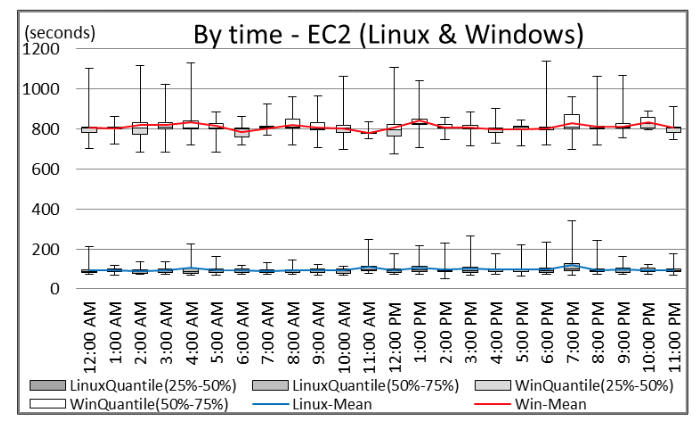
\includegraphics[scale=0.8]{vmstarttimes.png}
    \caption{EC2 VM startup time by time of the day (From\cite{mao2012performance})}
    \label{figure:vmstartuptimes}
  \end{center}
\end{figure}

\begin{flushleft}
  \begin{table}
    \begin{tabular}{ | l | l | l |}
      \hline
      Cloud & OS & Average VM startup time (in Seconds) \\ \hline
      EC2 & Linux & 96.9 \\ \hline
      EC2 & Windows & 810.2 \\ \hline
      Azure & WebRole & 374.8 \\ \hline
      Azure & WorkerRole & 406.2 \\ \hline
      Azure & VMRole & 356.6 \\ \hline
      Rackspace & Linux & 44.2 \\ \hline
      Rackspace & Windows & 429.2 \\ \hline
    \end{tabular}
    \caption{Average VM startup times (From\cite{mao2012performance})}
     \label{table:avgvmtime}
\end{table}
\end{flushleft}

Acquiring instances at the cost-optimal commitment level plays a central role for QoS versus cost management. This drives the motivation to build an efficient and flexible algorithm for provisioning and managing the VM instances.
\begin{flushleft}
  \begin{table}
    \begin{tabular}{ | L{2cm} | L{2cm} | L{2cm} | L{2cm} | L{2cm} | L{2cm} |}
      \hline
      Name & Upfrom Cost & Effective hourly cost & Effective montly cost & 1 year cost & 3 year cost \\ \hline
      On-demand & --- & 0.95 & 613.42 & 7361.04 & 22083.12 \\ \hline
      1-year reserved No upfront & 0.0 & 0.65 & 453.33 & 5439.96 & 16319.88 \\ \hline
      1-year reserved partial upfront & 2361.0 & 0.537 & 391.66 & 4699.92 & 14099.76 \\ \hline
      3-year reserved full upfront & 8580.0 & 0.327 & 238.34 & --- & 8580.0 \\ \hline
    \end{tabular}
    \caption{Instance Pricing Option for c4.4xlarge Linux instance type (prices in USD)}
     \label{table:cost}
\end{table}
\end{flushleft}

\begin{figure}[h]
  \begin{center}
    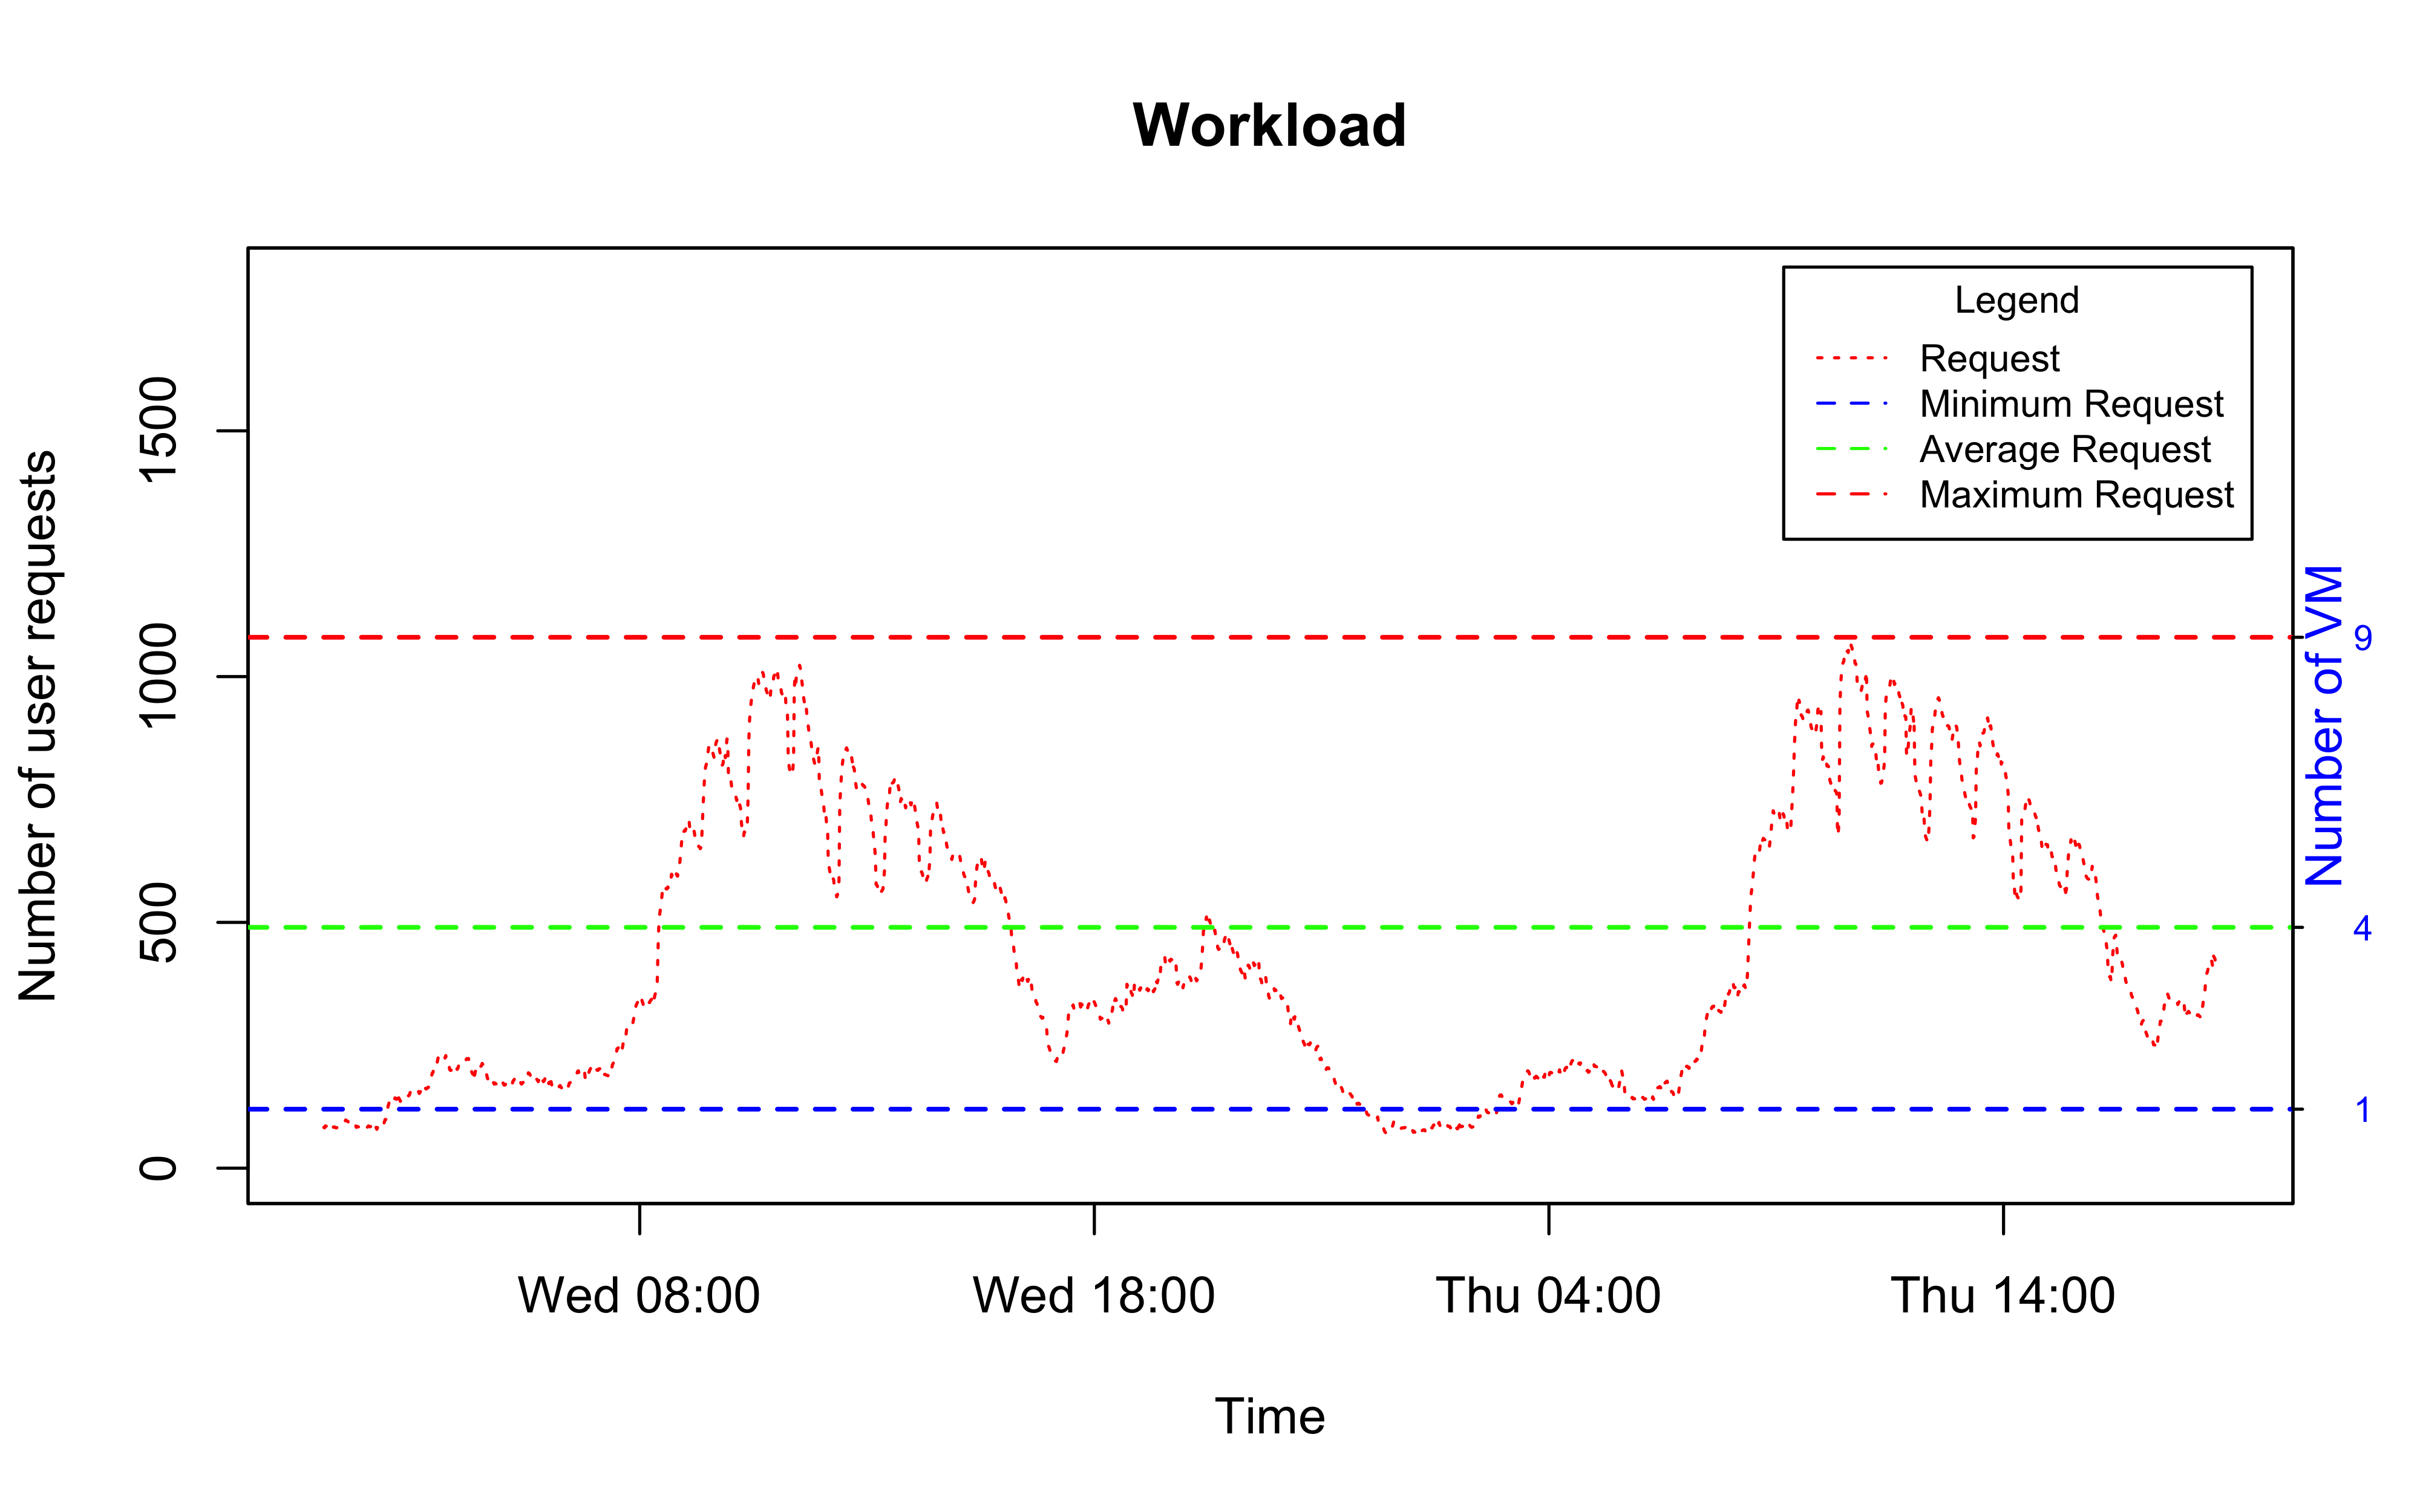
\includegraphics[scale=0.1]{workloadforsim}
    \caption{Sample Workload}
    \label{figure:citrixworkloadsample}
  \end{center}
\end{figure}


\section{Research Questions}

\label{sec:Research Questions}

Due to the challenges stated in the Section~\ref{sec:Motivation}, the goal of this thesis work is to design and implement an algorithm which can:

\begin{itemize}
  \item Compute the right number of VM resources required for the expected increase or decrease in workload.
  \item Ability to satisfies both application QoS and low operational cost by using different instance types provided by cloud service providers.
  \item Forecast future workload to proactively provision VM's to mitigate effects of delay in VM start and shutdown time overhead.
\end{itemize}

Based on this goal, four main research questions can be addressed and shall be answered within this thesis:

\begin{enumerate}
  \item What are the parameters to consider while computing the right number of VM resources required to satisfies QoS guaranties?
  \item What are the right VM instance types to use to achieve low operational cost?
  \item What kind of tool and technique can be used to accurately evaluate the performance and cost of the scaling algorithm without actual deployment on the clouds?
  \item What are the forecasting techniques which can be used to proactively provision VM's to mitigate effects of delay in VM start and shutdown time?
\end{enumerate}

\section{Contributions}
\label{sec:Contributions}
This thesis address the challenges mentioned in Section~\ref{sec:Motivation} with customer-oriented solution. At the beginning of this thesis, the state of the art techniques in customer-oriented solutions that do not employ cloud service provider involvement in the automated scaling of an application is investigated. On the light of these requirement, an proactive optimized threshold based\cite{lorido2012auto} automated scaling algorithm, named AppElastic, is proposed. AppElastic algorithm deals with the horizontal scalability\cite{vaquero2011dynamically} in IaaS mode. It address the trade-off problem between cost and QoS guaranties by employing very popular threshold based rules automated scaling algorithm. AppElastic employs time series forecasting to proactively compute the number of VM's needed to satisfy the QoS guaranties of the application. In this thesis the trade-off between the QoS and the cost is considered. Finally, to avoid the impact from arbitrary workload, AppElastic algorithm is designed to terminate the VM's which are nearing instance-hour.
\\
An experimental study on the performance evaluation of AppElastic algorithm at large-scale, a simulation based mode, called ElasticSim, is developed. ElasticSim evaluates the cost and performance of public IaaS clouds along with VM instances and diverse workload patterns. ElasticSim is fed with workload trace from Citrix audio/video conferencing application. The results show that optimizing the scalability thresholds and adopting proactive scalability can mitigate the resource provisioning overhead with cost benefits.




% remove this before sending it for the review.
%\bibliography{../handin}

\section{Structure}
\label{sec:Structure}
Following this chapter of introduction, the rest of this thesis is structured as follows:
\begin{itemize}
  \item Chapter~\ref{chap:Foundations} introduces the foundation knowledge necessary for this thesis with detailed explanations of the concepts and techniques that are used in AppElastic algorithm and ElasticSim simulation.
  \item Chapter~\ref{chap:RelatedWork} presents a few examples from related work that are either relevant to the field or have applied the tools and techniques mentioned above. It also includes discussions of the limitations of the work and the gap left for this thesis.
  \item Chapter~\ref{chap:ConceptSystemDesign} presents in detail the AppElastic algorithm for automated scaling, time series model for workload forecasting and shows the design of ElasticSim simulation system.
 \item Chapter~\ref{chap:ImplementationEvaluation} describes the implementation details of AppElastic algorithm, implementation of time series forecasting and  ElasticSim simulation environment. It also demonstrates the performance of AppElastic algorithm in ElasticSim simulation model and presents discussion about error rate of time series forecasting employed.
  \item Chapter~\ref{chap:DiscussionOutlook} summarizes the achievements of AppElastic automated scaling algorithm. It also outlines possible future work of this thesis.
  \item Chapter~\ref{chap:Conclusion} is the conclusion of the thesis.
\end{itemize}

\chapter{Foundations}
\label{chap:Foundations}
This chapter is dedicated for reviewing the concepts and technologies that enables rapid scalability of applications in cloud computing environment. The chapter starts by defining the concept of cloud computing, then in Section~\ref{sec:SLA}, service level agreement (SLA) in general is introduced and what it means for this thesis is presented. In Section~\ref{sec:ScalableSystems} a general scalability architecture of a typical cloud hosted application is presented. Finally  a brief introduction is presented on the theory of Time series analysis that will be used in this thesis for workload forecasting.

\section{Cloud Computing}
\label{sec:Cloud Computing}
Cloud computing\cite{mell2011nist} is a new paradigm for massively scalable systems and services. Cloud computing is an technology out of many foundational technologies especially networking, storage, virtualization, multi-tenant architecture, and distributed systems management. Cloud computing provides a broad array of web-services allowing users to access a wide range of capabilities on pay-as-you-go basis that previously required tremendous hardware and software investments.
\\
According to National Institute of Standards and Technology's NIST\cite{mell2011nist}, cloud computing is characterized by five essential characteristics, three service models.
\\
Five essential characteristics can be described as follows:
\begin{enumerate}
  \item On-demand \& self service: On-demand is an essential characteristic of cloud computing. Pay-as-you-go subscription models are associated with on-demand characteristic. Cloud computing provides its users computing power, storage, as needed without human interaction. Self-service of the On-demand service is offered through a dashboard that authorizes the users to control their resources. Cloud service providers allow its users to automate resource provisioning with application programming interfaces (APIs).
  \item Broad network access: Cloud computing resources can be to accessed over a wide varsity of network protocols and various types of clients ( e.g., tables, mobile, laptop and workstations ).
  \item Resource pooling: Cloud service providers offer their service, which is a pool of unassigned resources, to multiple customers in a multi-tenant model. The pool of resources is assigned and released based on the demand from customers.
  \item Rapid elasticity: Cloud resources can be elastically procured and released, to scale rapidly up and down based on the customer demand. To customers, cloud service provider appear to have unlimited resource pool.
  \item Measured service: Cloud service providers have the capability to monitor the cloud resources for better capacity planning, resource optimization and metering. Cloud service providers provides their customers capabilities to monitor the resource usage and control them.
\end{enumerate}
Three service models can be described as follows:
\begin{enumerate}
  \item Infrastructure as a Service (IaaS): Infrastructure cloud service providers offers to its customers capability to provision computing power, storage etc., in terms of VM's to deploy arbitrary software and operating system. Customer do not have access to underlying hardware infrastructure, but has controlled over operating system, storage and deployed application in the VM.
  \item Platform as a Service (PaaS): PaaS providers offers its customers capability to host applications on their platform. PaaS platforms provide a application an development environment, database services, execution environment, and web hosting. PaaS customers do not have control over underlying cloud infrastructure which include network, servers, operating systems, or storage, but have control over the application deployed and its configuration settings.
  \item Software as a Service (SaaS): SaaS providers offers its customers to use the application running on cloud infrastructure. The applications are accessed from various devices like web browser, table and mobile phone. The customers do not have control over the underlying cloud infrastructure, nor the individual application capabilities.
\end{enumerate}

\section{Service Level Agreement}
\label{sec:SLA}
SLA is a contract which defines the relationship between two parties: a service provider and its recipients. The contract describes the metrics by which the service quality are measured, and the penalties, if any, when agreed-upon service levels not achieved. Cloud hosted applications deals with two SLA contracts: First, SLA between cloud hosted application provider and cloud service providers. Second, between cloud hosted application provider and its customers. The SLA between cloud hosted application provider and cloud service providers is out of scope of this thesis. This thesis deals with SLA between cloud hosted application provider and its customers. This SLA is usually defined in terms of metrics by which the service is measured, for example, the response time, service availability etc., as quality of service (QoS) metrics.
\\
Service level objective (SLO) is specific measurable characteristic of the SLA such as availability, throughput, response time, or quality, used by the cloud hosted application to achieve the agreed SLA.
\section{Scalability of Applications}
\label{sec:ScalableSystems}
Scalability is the systems capability to accommodate the growing workload\footnote{\url{https://en.wikipedia.org/wiki/Scalability}}. Scalability is critical to the success of many organizations hosting application in cloud environment. An application can be scaled by adding or removing resources when needed. Scalable applications are capable of providing agreed-upon quality of service to meet the SLA on varying workloads.
\\
At a high level, resource can be added/removed using two methods:
\begin{itemize}
  \item \textbf{Horizontal scalability (scale in/out)} to add or remove VM instances to the system. An example might be to add more app server instances\cite{galante2012survey}.
  \item \textbf{Vertical scalability (scale up/down)} to add or remove resource like CPU, memory, network etc., to a single machine or VM\cite{galante2012survey}.
\end{itemize}
A typical scalable architecture of a cloud hosted application\cite{chieu2009dynamic} is illustrated in the Figure~\ref{figure:scalingarch}. The architecture design includes a front-end load balancer, an array of application servers with database servers, and a resource monitor with dynamic scaling algorithm. Use of load balancer such as Apache HTTP Load Balancer\footnote{https://httpd.apache.org/docs/2.4/mod/mod\_proxy\_balancer.html} will route user requests to application servers running as virtual machines. Load balancer has capability to dynamically add new application server instances. The application server enable the system to scale and provide better quality of service. The resource monitor is responsible for acquiring various application performance statistics, called as scaling indicator\cite{chieu2011dynamic}, which will be used by scaling algorithm to trigger and control scale-up or down the number of virtual machine instances. Before the emergence of cloud computing, scaling application is carried out by adding more physical servers to solve the problem of overload, which is a time consuming process. The emergence of cloud computing, starting more VM instances on-demand is in few seconds. Started instances are charged based on pay-as-you-go model, which helps in reducing the cost.
\begin{figure}[h]
  \begin{center}
    \includegraphics[scale=0.5]{scalingarch.png}
    \caption{Typical architecture of scalable applications in cloud(From\cite{chieu2009dynamic})}
    \label{figure:scalingarch}
  \end{center}
\end{figure}

\section{Time series Analysis}
\label{sec:Timeseries}
Understanding the nature of application workload is crucial in designing and provisioning current and future VM instances. Workloads on the application are often driven by repeatable business behavior and exhibit temporal and spatial correlations. Application workloads behave in frequent and repeatable patterns. Such behavior patterns make some workload variations predictable\cite{mao2011auto}. Time Series Analysis techniques are used to identify patterns in temporal data (know as time series), using methods such as smoothing and curve fitting, and autocorrelation\cite{timeseriesdefinition}. In the following subsections, first review techniques used to identify patterns in time series data, and then general class of models that can be used to represent time series data and generate predictions are introduced.
\subsection{Time series Data}
\label{sub:Timeseriesdata}
Time series data is sequences of measurements that follow non-random orders\cite{shumway2006time}. Unlike the analyses of random samples of observations that are used in general statistics, the analysis of time series is based on the assumption that successive values in the data represent consecutive measurements taken at equally spaced time intervals. A number of different notations are in use for time-series analysis. A common notation specifying a time series \(X_{t}\) that is indexed by the natural numbers\cite{timeseriesdefinition}:
\begin{equation}
  X_{t}={X_{1},X_{2}, ...}
\end{equation}
\\
Two main goals of time series analysis are as follows:
\begin{enumerate}
  \item Identifying the nature of the phenomenon represented by the sequence of observations.
  \item Forecasting, predicting future values of the time series variable.
\end{enumerate}
Both of these goals require the pattern of observed time series data to be identified and formally described. Once the pattern is identified it can be used to predict future events. In order to successfully achieve these tasks it is necessary to assume a-priori structure of the time series. If \(X_{t}\) is completely arbitrary random variables, then \(X_{1},.....,X_{n}\) constitute a single observation from a completely unknown distribution on \(\mathbb{R}^n\)\cite{timeseriesdefinition}. Drawing conclusion about these random series is impossible. Hence, the structure of the time series is assumed to be stationary. Stationary series does not change when shifted in time. Consequently, parameters such as the mean and variance, if they are present, also do not change over time\footnote{https://en.wikipedia.org/wiki/Stationary\_process}.
\theoremstyle{definition}
\begin{definition}{}
The time series \(X_{t}\) is strictly stationary\cite{timeseriesdefinition} if the distribution of the vector \((X_{t},X_{t+1},...,X_{t+k})\) is independent of \(t\) for every \(k \in \mathbb{N}\).
\end{definition}

\begin{definition}{}
A time series is said to be weakly stationary\cite{timeseriesdefinition} if:
\begin{enumerate}
  \item \(mean(X_{t}) = \mu\)
  \item \(Covariance( X_{t},X_{t+k}) = \gamma_{k} \)
\end{enumerate}
where \(\mu\) is constant and \(\gamma_{k}\) is independent of \(t\).
\end{definition}
\begin{definition}{}
The sequence \((X_{1},X_{2},....,X_{t})\), consisting of independent (or uncorrelated\footnote{If \(Covariance(X_{t}, t ) = 0\), we say that \(X_{t}\) and \(t\) are uncorrelated}) random variables with mean 0 and variance \(\sigma^2\) is called White noise.
\end{definition}

\subsection{ARIMA}
\label{sub:ARIMA}
 Autoregressive integrated moving average (ARIMA)\cite{box2015time} model is a generalization of an autoregressive moving average (ARMA)\cite{whitle1951hypothesis} model. To understand ARIMA, concept of ARMA has to be defined first.
\subsubsection{ARMA}
\label{subs:ARMA}
Linear regression models attempt to explain a variable by the sum of a linear function of explanatory variables and a noise variable. ARMA processes are a time series version of linear regression, where the explanatory variables are the past values of the time series and the added noise is a moving average process.

The autoregressive process of order \(p\) is denoted \(AR(p)\), and defined by\cite{timeseriesdefinition}:
\begin{equation}
  X_{t} = \sum_{r=1}^{p} \phi_{r} X_{t-r} + \epsilon_{t}
\end{equation}

where \(\phi_{1},...,\phi_{r}\) are fixed constants, and the sequence \(\epsilon_{t}\) is  independent (or uncorrelated) random variables with mean 0 and variance \(\sigma^2\).

The AR process order 1 i.e \(AR(1)\), is defined as\cite{timeseriesdefinition}:
\begin{equation}
  X_{t} = \phi_{1} X_{t-1} + \epsilon_{t}
\end{equation}

The moving average process of order \(q\) is denoted \(MA(q)\) and defined by\cite{timeseriesdefinition}:

\begin{equation}
  X_{t} = \sum_{s=0}^{q} \theta_{s} \epsilon_{t-s}
\end{equation}

where \(\theta_{1},\theta_{2},...,\theta_{q}\) are fixed constants and \(\theta_{0}=1\), and the sequence \(\epsilon_{t-s}\) is a independent random variables with mean 0 and variance \(\sigma^2\).

Based on $AR$ and $MA$ process defined above, the autoregression moving average process, \(ARMA(p,q)\) is defined as\cite{timeseriesdefinition}:
\begin{equation}
  X_{t} -  \sum_{r=1}^{p} \phi_{r} X_{t-r} = \sum_{s=0}^{q} \theta_{s} \epsilon_{t-s}
\end{equation}
where again $\epsilon_{t} $ is white noise\cite{timeseriesdefinition}. This process is stationary for appropriate $\theta,\phi$.

Before defining ARIMA, the concept of differencing should be defined. Differencing is a method to transform a non-stationary time series into a stationary one. This method is particularly studied in combination with ARMA modeling. Differencing is defined as\cite{timeseriesdefinition}:
\begin{equation}
  X_{t} = \nabla Y_{t} = Y_{t} - Y_{t-1}
\end{equation}
where the non-stationary series $Y_{t}$ is transformed to stationary by applying successive differencing operation. Order of differencing $d$ is the number of successive differencing operation applied and is denoted as $\nabla^d$\cite{timeseriesdefinition}.

ARIMA process is defined as\cite{timeseriesdefinition}:
\begin{definition}{}
A time series $X_{t}$ is an $ARIMA(p,d,q)$ process if $\nabla^d X_{t}$ is a stationary $ARMA(p,q)$ process.
\end{definition}

In other words, the time series $X_{t}$ is an $ARIMA(p,d,q)$ process if there exist polynomials $\phi,\theta$ of degree $p,q$ and a white noise series $\epsilon_{t}$ such that the time series $\nabla^d X_{t}$ is stationary\cite{timeseriesdefinition}. Additional ``I'' in $ARIMA$ is for integrated, hence $ARIMA$ process is called as integrated ARMA process.

Identification, Estimation and Forecast forms main goals of $ARIMA$ modeling. This process are summarized below:
\begin{enumerate}
  \item Identification: The input series for ARIMA needs to be stationary, that is, it should have a constant mean, variance, and autocorrelation through time. To possibly identify a $ARIMA$ model that the series transformations into a stationary series. At this stage autoregressive $p$ and moving average $q$ order in ARMA model for the stationary series are identified. In practice, the values of the $p$ or $q$ parameters will not be greater than 2.
 \item Estimation and Forecasting: In Estimation process, the parameters are estimated, so that the sum of squared residuals is minimized. The estimation process is performed on transformed data. The estimates of the order are used in the Forecasting to calculate new values of the series and confidence intervals for those predicted values are calculated. Before the forecasts are generated, the series needs to be integrated so that the forecasts are expressed in values compatible with the input series.
\end{enumerate}
$ARIMA$ modeling process can be automated using various software modeling tools that apply methodology like Box-Jenkins method to find the right order for the $ARIMA$ model. R the software environment for statistical computing includes an \(arima\) function, which is used to fits an $ARIMA$ model to a univariate time series. The forecast package in R can automatically select an ARIMA model from models fitted by \(auto.arima()\) function for a input time series. The forecasted time series will include predicted values and standard errors (se). In this thesis, ARIMA forecasting techniques are employed for predicting future workload to proactively scale cloud hosted applications.
\section{Summary}
\label{sec:Summary}
Section~\ref{sec:Cloud Computing} introduced the basic definition of cloud computing and its service models. In section~\ref{sec:SLA}, SLA was formally defined. Section~\ref{sec:ScalableSystems} defined scalability of cloud hosted systems and depicted typical scalable applications in cloud in Figure~\ref{figure:scalingarch}.
Section~\ref{sec:Timeseries}, formally defined the concept of time series analysis and ARIMA process. At the end of this chapter it was defined how ARIMA process is used to generate forecasts.


\chapter{Related Work}
\label{chap:RelatedWork}
In this chapter, some related work of this thesis is presented. The first section gives the classification of elasticity mechanisms as proposed by \cite{galante2012survey} \cite{dawoud2013scalability} \cite{lorido2012auto}. In the second section the state of the art techniques in autoscaling such as time series forecasting and threshold based mechanism which is investigated and applied in this thesis are presented. Finally an analysis and evaluation of the work done on the state of the art simulation methods in cloud computing research is presented.

\section{Classification of elasticity mechanism}
\label{sec:Classification of elasticity mechanism}
Classification of various autoscaling techniques based on the elasticity mechanism will help in classifying state of the art autoscaling techniques. This section provides a comprehensive study about various elasticity mechanism available today. In the first part of this section, classification of various elasticity mechanism  is presented which is proposed by \cite{galante2012survey} \cite{dawoud2013scalability} \cite{lorido2012auto}. The classification created here for the purpose for this thesis is based upon the works of \cite{galante2012survey} \cite{dawoud2013scalability} \cite{lorido2012auto}. Galante et al.\cite{galante2012survey} purposed a classification of elasticity mechanism based on four characteristics:
\begin{enumerate}
  \item Scope
  \item Policy
  \item Purpose
  \item Method
\end{enumerate}
Classification purposed by the authors can be illustrated in Figure~\ref{figure:elasticclassification}. This classification is based on various studies done on academics research and cloud service providers recommendation. The classification proposed by Galante et al.\cite{galante2012survey}, calls Horizontal scaling as replication of virtual machines, and Vertical scaling as re-dimensioning of virtual machines.

\begin{figure}[h]
  \begin{center}
    \begin{forest}
   for tree={grow=0,parent anchor=east, child anchor=west, edge path={\noexpand\path[\forestoption{edge}] (\forestOve{\forestove{@parent}}{name}.parent anchor)-- +(0:2mm)|-(\forestove{name}.child anchor)\forestoption{edge label};}}
  [Elasticity
    [Scope
        [Infrastructure]
        [Application]
    ]
    [Policy
        [Manual]
        [Automatic
            [Reactive]
            [Proactive]
        ]
    ]
    [Purpose
        [Performance]
        [Increase Elasticity]
        [Cost]
        [Energy]
    ]
    [Method
        [Horizontal]
        [Vertical]
        [Migration]
    ]
  ]
  \end{forest}
    \caption{Classification of Elasticity (From \cite{galante2012survey})}
    \label{figure:elasticclassification}
  \end{center}
\end{figure}

\section{State of Art}
\label{sec:State of Art}
In recent years, lots of state-of-the-art\cite{lorido2012auto} techniques for horizontal scalability have been successfully developed in research institutes and industries. These developed scalability solutions have turned out to be very helpful and valuable tools in scientific researches as well as commercial products. In this section diverse related work is reviewed in order to present the state of the art auto scaling techniques in clouds.

\subsection{Threshold Based Rules}
\label{sub:Threshold Based Rules}
Galante at el.\cite{galante2012survey} defines the threshold or rule based mechanism for horizontal scaling as a Rule-Condition-Action mechanism. Rules consists of set of conditions upon meeting these conditions appropriate scaling actions are trigged. Every condition consists of performance metric from the system which is compared against a threshold. The information about the performance metric values are provided by the infrastructure monitoring system\cite{lorido2012auto}. Each threshold is defined by the user and its composed of two parameters: an upper threshold and a lower threshold for each performance metric\cite{lorido2012auto}. The scaling action will scale the resource based on the  type of scaling. For horizontal scaling, the user will define fixed number VM instances to create or destroy, but for vertical scaling user will define the amount to resources of a particular resource type to be added or removed to the VM. An example for a threshold based rule is: add two instance when the number of user sessions exceeds  100 user sessions per instance\cite{lorido2012auto}.
Amazon AWS offers horizontal scaling mechanism called Auto Scaling as part of its EC2 service\cite{AmazonAutoScale}. The solution is based on a concept called Auto Scaling Groups(AGS)\cite{AmazonAutoScale}. AGS consists of a set of instances that can be used by an application. Amazon Auto Scaling mechanism uses an automatic-reactive approach\cite{galante2012survey}. Foreach AGS, rules are defined to add or release predefined number of instances\cite{AmazonAutoScale}.
\\
RightScale\cite{Rightscale}, a popular cloud management solution for managing cloud infrastructure across multiple IaaS providers, provides horizontal autoscaling mechanism which uses a simple democratic voting to scale up or down\cite{galante2012survey}. Running VM instance participate in the process of voting and scaling action is taken based on majority of votes. After each scaling action a cooldown time is introduced where in no scaling action will be taken\cite{lorido2012auto}. This cooldown time is provided to prevents the algorithm from continually allocating resources as new instances boot\cite{kupferman2009scaling}. Rightscaling algorithm is highly dependent on user-defined values for threshold and cooldown time, if these values are not optimally tuned it can lead to rapid starting and termination of machines due to rapid spikes in workload. Kupferman et al.\cite{kupferman2009scaling} extends the RightScale algorithm with a concept called smart kill. The authors\cite{kupferman2009scaling} considers the fact that machines are charged by cloud service providers in hourly basis. This approach does not terminate the instances even if the load is low and the instance is not required, because the instance will be paid for entire hour, and there no reason to terminate the instance before the finish of instance hour\cite{kupferman2009scaling}.
\subsection{Reinforcement Learning}
\label{sub:Reinforcement Learning}
Reinforcement learning is an automatic decision making process which is applicable for autoscaling mechanism\cite{lorido2012auto}. Reinforcement learning\cite{Reinforced} is defined as an automated approach to goal oriented learning and decision making. Learning is done through directed interaction between agent and its environment. Reinforced learning process can be illustrated from the Figure~\ref{figure:reinforced}. Agent is the  decision-maker that learns from its experience to make best action to execute for each state of the environment and always try to maximize the reward\cite{Reinforced}. In terms of autoscaling problem, the autoscale algorithm is the agent that interact with the application environment. This will decide whether to add or remove (actions) VM instances to the system depending on the workload, performance or other set of metic(state). This process always tries to minimize the values like response time, cost (reward) etc.
\begin{figure}[h]
  \begin{center}
    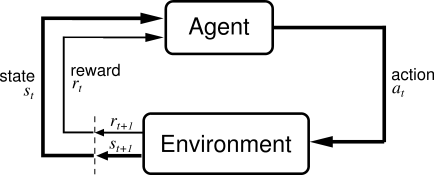
\includegraphics[scale=0.9]{reinforced.png}
    \caption{The agent-environment interaction in reinforcement learning (From\cite{Reinforced})}
    \label{figure:reinforced}
  \end{center}
\end{figure}
Yazdanov et al.\cite{yazdanov2013vscaler} proposes a concept called VScaler, which is a framework implementing autonomic resource allocation using reinforcement learning. Here authors model the  states as number of VM's running, actions are amount of VM's which can be added, removed or maintained\cite{yazdanov2013vscaler}, and utilization of the VM's as reward function. In works of\cite{barrett2013applying},\cite{dutreilh2011using},\cite{rao2009vconf} reward function is studied in perspective of cost of VM machines and  SLO violations.
\\
Although reinforcement learning methods for autoscaling look promising,\cite{lorido2012auto} points out several problems:
\begin{itemize}
  \item Curse of dimensionality problem\cite{yazdanov2013vscaler}: The size of the state space grows  exponentially with each added new state variable. Yazdanov\cite{yazdanov2013vscaler} estimates there will be 10240 states if VM's with two resource parameters, 10 different values for each parameter and 10 actions for every state.
  \item Large learning time \& bad initial performance: Agent in reinforcement learning approach learns about its environment by visiting each state-action pair. Therefore learning process time depends on the size of state-action space. Large initial learning process leads poor initial performance of the reinforcement algorithm.
\end{itemize}
In order to improve the bad performance Yazdanov\cite{yazdanov2013vscaler} proposed a reinforcement learning model with parallel learners to speed up the agent learning process.
\subsection{Time-series Analysis}
\label{sub:Time-series Analysis}
Time series analysis uses historical data to predict future workloads. Time series are used in many domain such as engineering, finance, economics and bioinformatics, to represent changes in the system over time. Time series analysis and forecasting methods are generally used in proactive autoscaling mechanisms. In 2012 Herbst\cite{herbst2012workload} published his diploma thesis from University of Wuerzburg on workload classification and forecasting. This work presents a detailed survey of various methods in time series analysis and forecasting. The author made a detailed survey and grouping of various time series and  forecasting based on their strengths and weakness. Based on this comparative study a dynamic approach know as WorkloadClassificationAndForecasting (WCF)\cite{herbst2012workload} is developed. WCF\cite{herbst2012workload} has capability to dynamically create time series model for a given time series data. The author has implements WCF as Java based software\footnote{\url{https://github.com/NikolasHerbst/WCF}} which is used extensively in research community. Here\cite{herbst2012workload} it also proves from experimental setup that the effect of workload forecasting in proactive resource provisioning can avoid 52\% to 70\% SLA violations. A subset of the survey on time series forecasting published by the authors\cite{herbst2012workload} is presented in the Table~\ref{table:tssurvey}.
\\
In work done by Roy et al.\cite{roy2011efficient}, authors proposed autoscaling by static threshold based method in combination with workload forecasting. Here the authors have used second order autoregressive moving average method (ARMA) for workload forecasting and combines with response time and server utilization as autoscaling thresholds. Further, Islam et al.\cite{islam2012empirical}, proposed a proactive prediction based autoscaling strategies using Neural Network and Linear Regression.
\begin{flushleft}
  \begin{table}
    \begin{tabular}{ | L{2cm} | L{2cm} | L{2cm} | L{2cm} | L{2cm} | L{2cm} |}
      \hline
      Name & Forecast horizon & Historical data & Strengths & Weakness & Suitable for use case \\ \hline
      Naive forecasting  & 1-2 points & Single previous observation & No historical data required & No use in proactive autoscaling as the prediction horizon is too small & Constant arrival rate \\ \hline
      Moving average (MA) & 1-2 points & Two consecutive observations & Simplicity & Sensitivity to trends and seasonal components & Constant arrival rate with low white noise \\ \hline
      ARMA & less than 5 points & Small number of historical data & Trend estimation is possible and has fast forecast performance & No season component in included model, only positive time series & Time series with some noise and trend\\ \hline
      ARIMA\cite{box2015time} & more than 5points & At least 3 periods in time series data & Capturing noise, trend and season component & Complex modeling & Times series with seasonal component and moderate noise level\\ \hline
    \end{tabular}
    \caption{Table of Forecast Strategies and their Properties (From\cite{herbst2012workload})}
    \label{table:tssurvey}
\end{table}
\end{flushleft}

\subsection{Combined Approach}
\label{sub:Combined Approach}
In the recent years, the above mentioned scaling mechanism has be combined and studied to develop an efficient proactive scaling mechanisms. These methods are widely researched and published by Roy et al.\cite{roy2011efficient}, Sharma\cite{sharma2011cost}, AzureWatch\cite{Azurewatch}, Gong\cite{gong2010press}, Nguyen\cite{nguyen2013agile}. Roy et al.\cite{roy2011efficient} in their paper developed a proactive look-ahead technique for workload forecasting using ARMA time series forecasting strategy working in combination with threshold rules defined on utilization of each VM (taking mean value of utilization). The authors objective was to minimize resource usage, satisfy the application QoS and keep operational cost low\cite{galante2012survey}.
\\
PRESS was developed by Gong\cite{gong2010press} which uses signal processing techniques to identify patterns in the workloads. These identified patterns are then used to predict future workload. PRESS fall back to statistical state machine based approach if there were no pattern emerged from the historical workload. This approach helps application maintain SLA guarantees with minimum resource allocation. Nguyen\cite{nguyen2013agile} developed a concept called AGILE, which is a proactive scaling mechanism uses wavelet transformation for workload forecasting\cite{nguyen2013agile}. AGILE uses a concept called resource pressure which is a ratio of resource usage for scaling the resources.
\\
AppElastic algorithm developed in this thesis tries to extent the concept of\cite{roy2011efficient}. In contrast to  Roy et al.\cite{roy2011efficient}, AppElastic algorithm uses ARIMA forecasting. ARIMA forecasting models are generally used to predict future workload point for more than five mins (as shown in the Table~\ref{table:tssurvey}). It also differs from \cite{roy2011efficient} by using number of active sessions per VM instances as threshold for scaling.

\section{Cloud Simulation Methods}
\label{sec:Cloud Simulation Methods}
Evaluating the effectiveness of a autoscaling algorithm is often realized over the time spent in production system operating under hight workloads\cite{AlexanderSim}. When working with production system workload trace, which generally spans over multiple months, empirical evaluation of autoscaling algorithms on real-time production system workload trace is infeasible. To address this challenge, academic community has put forward several approaches to simulate the autoscaling algorithm evaluation.
\\
Through these simulation approach systems can be evaluated from two perspectives one from IaaS cloud perspective and other from the application perspective. Pucher\cite{AlexanderSim} in his blog post summarizes a list of popular simulation software widely used by the research community. Pucher\cite{AlexanderSim} classifies simulation software developed in academia into Infrastructure Simulators and Application-perspective cloud simulators. A survey of these simulators presented by Pucher\cite{AlexanderSim} is presented below.
\subsection{Infrastructure Simulators}
\label{sub:Infrastructure Simulators}
Infrastructure simulators are used to simulate cloud computing infrastructure and services. It is widely used among the cloud computing research fields such as fault-tolerance, scalable computing such as MapReduce\cite{dean2008mapreduce} etc. Two widely used infrastructure simulators are listed below:
\begin{itemize}
  \item Cloudsim\cite{calheiros2011cloudsim}: Cloudsim is used for modeling, simulation, and experimentation of emerging Cloud computing infrastructures and application services. Cloudsim provides modeling and simulation features for large scale Cloud computing data centers\cite{Cloudsim}, virtualized server hosts\cite{Cloudsim}, data center network topologies and message-passing applications\cite{Cloudsim} and much more.
  \item GreenCloud\cite{kliazovich2012greencloud}: GreenCloud is used to develop simulation of monitoring of resource, resource allocation, workload scheduling and network infrastructures\cite{Greencloud}. GreenCloud simulate cloud computing resources such as CPU, memory, storage and networking resources. It also supports energy models of all resource types and provides a GUI for its users. GreenCloud is widely used among the research communities studying energy aware cloud computing systems.
\end{itemize}

\subsection{Cloud Hosted Application Perspective Simulators}
\label{sub:Cloud Hosted Application Perspective Simulators}
Cloud hosted application simulators are designed to simulate cloud computing services in terms of cloud user or cloud application perspective. It hides the underlying details of the cloud infrastructure and focus on application perspective metrics such as cloud cost, the number of created VMs, VM utilization, horizontal and vertical scaling of cloud resources\cite{kim2015pics}. One of the widely used simulators developed at Univeristy of Virginia know as Public Cloud IaaS Simulator (PICS)\cite{kim2015pics} is described below:
\begin{itemize}
  \item PICS: PICS enables the cloud user to evaluate the cost and performance of public IaaS clouds along with VM instances and storage service, resource scaling, job scheduling, and diverse workload patterns\cite{kim2015pics}. PICS focus on capabilities like: cloud cost, the number of VMs created, VM utilization, horizontal and vertical scaling of VMs, and job deadline satisfaction rate\cite{kim2015pics}.
\end{itemize}

Authors of \cite{kim2015pics} provide a comparative study of various cloud simulators capabilities and its applicability in cloud simulation experiments. Table~\ref{table:simtable} summarizes the capability comparison of various simulators which is originally presented in \cite{kim2015pics}.

\begin{flushleft}
  \begin{table}
    \begin{tabular}{ | L{5cm} | L{5cm} | L{5cm} | }
      \hline
      Simulators & Capabilities & Drawbacks \\ \hline
      Cloudsim\cite{Cloudsim} & VM management in datacenters, physical resource management and scaling in datacenters, Federated cloud management. & Limited or no autoscaling simulation support. \\ \hline
      GreenCloud\cite{kliazovich2012greencloud} & Physical resource management in datacenters, power consumption management in datacenters. & No autoscaling simulation. No billing management or cost optimization. \\ \hline
      Public Cloud IaaS Simulator (PICS)\cite{kim2015pics} & Job scheduling in cloud, Horizontal and Vertical autoscaling, billing and cost management. & Difficulty in modeling performance uncertainty of real public clouds. \cite{kim2015pics} \\ \hline
    \end{tabular}
    \caption{Simulation Capabilities of Existing Cloud Simulator and PICS (Table taken from \cite{kim2015pics})}
     \label{table:simtable}
\end{table}
\end{flushleft}

\section{Summary}
\label{sec:Summary}
Section~\ref{sec:Classification of elasticity mechanism} introduced a classification of elasticity mechanisms introduced by \cite{galante2012survey}. In this concept of classification the AppElastic algorithm was also classified to be customer oriented approach to elasticity which is a proactive automatic policy based horizontal scaling mechanism.
\\
Section~\ref{sec:State of Art} gives various state-of-the-art techniques used in horizontal autoscaling. Some of the state-of-the-art techniques introduced such as, Threshold based and Time-series forecasting provides a promising techniques for horizontal scalability. These techniques will also be used later. However, there still exists a space for an effective and easy to use approach which efficiently scales the resources horizontally using threshold based rules combined with workload forecasting. These techniques will also be used later and this is the main focus of this thesis.
\\
Secion~\ref{sec:Cloud Simulation Methods} collects some comparison work from cloud computing simulation research. Few widely used cloud simulators are evaluated based on the features and its capabilities. The simulation methods proposed are specific to certain specific use cases. Cloudsim and GreenCloud simulator are incompatible with horizontal scalability. However, PICS provides necessary feature for the horizontal scalability,  but it lacks some of the features necessary for this thesis such as cost calculation and workload forecasting. Nonetheless PICS provided a good starting point in designing ElasticSim. The design of custom simulator ElasticSim is covered in later chapters.


\chapter{Concept and System Design}
\label{chap:ConceptSystemDesign}
As it was stated in the introduction chapter of Section 1.1, the major research goal of this thesis is the construction of an automated solution for horizontal scalability problem which meets the SLA guarantees along with cost benefits. The approach taken to achieve this goal is presented in this chapter. This approach uses threshold based rules to scaling virtual machines horizontally by applying workload forecasting. To enable workload forecasting, ARIMA time series forecast strategy is applied periodically. The AppElastic autoscaling algorithm presented in this chapter works in collaboration with workload forecasting to proactively scale the system. This chapter revolves around the idea of ensuring SLA requirements by workload forecasting and scale the resource by threshold based rules.
\\
The proposed AppElastic algorithm is explained in three folds. First in Section~\ref{sub:AppElastic without look-ahead} an algorithm is developed as reactive provisioning solution to meet the SLA requirements for any workload. Next in Section~\ref{sub:AppElastic with look-ahead} algorithm is extended to provide a proactive scaling to solve the problem with VM provisioning latency. Finally, at the end of the Section~\ref{sub:AppElastic with look-ahead} complete AppElastic algorithm is presented.
\section{Assumptions and Limitations}
\label{sec:Assumptions and Limitations}
It is safe to assume that software monitoring services  such as Nagios~\cite{josephsen2007building} is able to monitor constantly and report the workload as user request arrive to the system. In this case time series forecast system can be applied to predict future workload points. Concerning the approach taken in this thesis, the input to time series based forecasting strategy assumes to be a time series of number of user requests arriving to the system. The time series forecasting mentioned in the following section is not meant to be applied on resource utilization, response time or any other throughput values.
\\
Going further in this thesis Amazon AWS is considered as a cloud service provider. As it was presented in table~\ref{table:cost}, Amazon AWS provides two types of instances, pay-per-use on-demand instances(ODI) and one-time/partial prepaid reserved instances(RI). These various instance purchasing option and cost model is used as an example in this thesis.
\\
Any time series forecasting strategy has an inheriting uncertainty due to unforeseeable system workload changes. It is obvious that system under drastic events can not be forecasted solely based on historical data \cite{herbst2012workload}. Influence of unplanned events can cause anomalies in the scaling decision that can be detected and analyzed afterwards.

\section{SLA Violations}
\label{sec:SLA Violations}
SLA aware provisioning is an important aspect for the service consumers and SLA violations are used to trigger scaling. Most of the works presented in related work chapter use SLA violations to trigger scaling either using proactive or reactive methods. SLA aware solutions are limited to providing some guarantees with respect to the service response time. In the scope of this thesis, SLA guidelines were given by industry partner Citrix Online Dresden. Based on extensive research conducted by Citrix Online team, SLA violations for its audio/video server were defined in terms of number users being served by audio/video servers. It was identified that, to meet SLA agreement for all its users, each server should server not more than 120 user in any given time. If server assigned more than 120 users, SLA agreement was being violated.

\section{AppElastic Algorithm}
\label{sec:AppElastic Algorithm}

\subsection{AppElastic without look-ahead}
\label{sub:AppElastic without look-ahead}

In this section AppElastic algorithm is introduced without the feature of workload forecasting. Algorithms strengths and weaknesses will also be discussed. In order to understand the algorithm better, Table~\ref{table:paratable} list the input parameters of the algorithm. First of all, the IaaS cloud providers has specific billing period for its instances. This value is specified with the parameter $B_{p}$. This billing period varies based on the cloud service providers. For example, Amazon AWS charges its customer instances in hourly basis\footnote{https://aws.amazon.com/ec2/pricing/}. In addition, users need to specify the time required to startup and shutdown a virtual machine as in $T_{startup}$ and $T_{shutdown}$ respectively. As explained in Chapter \ref{chap:Introduction}, each virtual machines has unpredictable long startup time\cite{mao2012performance}. This varied startup time are necessary to consider in AppElastic algorithm since it has a considerable delay in provisioning the VM for the application users to fulfill SLA requirements. VM shutdown time generally depends on the graceful shutdown of the application running inside VM and this value has to be specified based on experiments done based on specific application. In the scope of this thesis, industry partner Citrix online provided the VM instance startup time as 5 mins and, 15 mins for migrating its user  and completely shutdown the virtual machines.
\\
As it was defined, AppElastic algorithm is based on threshold based rules. AppElastic algorithm takes number of user session per VM instance as threshold specified by the parameter \( U_{i} \). This threshold is used for triggering scaling of VM. This threshold is determined by QoS demand requirements as per SLA. The pseudo code of the algorithm is given in \textit{Algorithm}~\ref{algo:appelasticwithoutlookahead}. Output values from  \textit{Algorithm}~\ref{algo:appelasticwithoutlookahead} are as shown in Table~\ref{table:outputtable}. It give two type of output, one is the usage of each VM instance through $VM_{usage}^{i}$ and cost associated with this usage in $VM_{cost}^{i}$. Algorithm is started after application is deployed and keeps running until application is completed. Scaleup is triggered when it observe the user requests growing above the specified threshold or scale down if the billing period of VM is ending and number of user session are below specified threshold.
\\
The algorithm applies an automatic reactive scaling mechanism similar to mechanisms applied by Amazon Auto Scale and Rightscale\cite{han2012lightweight}. The threshold based scaling need no prior knowledge about the application. Each time VM instances are scaled its load balancing server automatically redistributes incoming user request to new created instances\cite{han2012lightweight}. This algorithm tries to provide best service for all of its application users by creating as much VM instances needed. This algorithm is effected by the VM startup time, since there is an overhead in VM startup time, VM's cannot be made available by the scaling algorithm to the application users. As show in the Figure~\ref{fig:slaviolationfig}, due to a sudden increase in incoming user requests the scaling algorithm starts adding new machines, since VM has considerable startup time users were not served at this time and SLA is violated. To solve this problem, we need a mechanism to predict user request for certain period, so that algorithm can look-ahead in time and add new VM instances which server all upcoming user requests without violating SLA.

\RestyleAlgo{boxruled}
\LinesNumbered
\begin{algorithm}[H]
 \KwIn{  \( U_{i} \),\( B_{p} \),\( T_{start} \),\( T_{shutdown} \)}
 \KwOut{$VM_{usage}^{i}$, $VM_{cost}^{i}$}
 \While{until application is active}{
  \tcc{user request \( r_{i} \) at time \(t_{i}\)}
  \(r_{i}  \) = getUserRequest()\;
  \tcc{machines \( n_{i} \) required at time \( t_{i} \)}
  \( n_{i} = r_{i} / U_{i} \)\;
  \tcc{machines already running \( m_{i} \) at time \( t_{i} \)}
  \( m_{i} = getRunningVmInstanceCount() \)\;
  \uIf{\( n_{i} > m_{i} \)}{
    \tcc{Add more machines}
    \(newMachinesToStart =  n_{i} - m_{i}\)\;
    \lFor{ i=1 \emph{\KwTo} newMachinesToStart }{
    \tcc{New VM takes \( T_{start}\) mins to start}
    start new VM instance
    }
   }
   \uElseIf{\( n_{i} < m_{i} \)}{
    \(machinesToShutdown =  m_{i} - n_{i}\)\;
    \tcc{Stop machine before billing period to avoid billing to next hour and machines take \( T_{shutdown}\) mins to shutdown. Only stop machines which are nearning billing period.}
    \lFor{ i=1 \emph{\KwTo} machinesToShutdown }{ Stop VM instance ending billing period }
  }
 }
 \caption{AppElastic Algorithm without look-ahead}
 \label{algo:appelasticwithoutlookahead}
\end{algorithm}

\begin{center}
  \begin{table}
    \begin{tabular}{ | L{6cm} | L{6cm} |}
      \hline
      Parameter & Description \\ \hline
      \( U_{i} \) & Number of user session a single instance can accommodate  \\ \hline
      \( B_{p} \) & Billing period of instance as per cloud service provider policy \\ \hline
      \( T_{start} \) & Time taken for a VM and its application to start  and update its states if necessary  \\ \hline
      \( T_{shutdown} \) & Time taken for VM instance shutdown\\ \hline
    \end{tabular}
    \caption{List of input parameters to AppElastic algorithm}
     \label{table:paratable}
\end{table}
\end{center}

\begin{center}
  \begin{table}
    \begin{tabular}{ | L{6cm} | L{6cm} |}
      \hline
      Parameter & Description \\ \hline
      $VM_{usage}^{i}$ & Usage of each $VM_{i}$ in minutes  \\ \hline
      $VM_{cost}^{i}$ & Cost of $VM_{i}$ for its usage \\ \hline
    \end{tabular}
    \caption{List of out values from AppElastic algorithm}
     \label{table:outputtable}
\end{table}
\end{center}


\subsection{AppElastic with look-ahead}
\label{sub:AppElastic with look-ahead}
\subsubsection{Workload Forecasting Technique}
\label{subs:Workload Forecasting Technique}
To illustrate the process of time series modeling, workload from audio/video conferencing server logs is analyzed. To analyze the workload using time series model, the user requests are captured in the form of discrete time series values. Actual workload to the algorithm is be depicted in the Figure~\ref{figure:sampleworkload}. As discussed earlier, each point represents the total number of requests for each minute. The workload is captured every minute, hence the scaling decision would be taken at the interval of one minute and thus the forecast has to be done for next minutes. For  modeling of time series and forecasting workload, ARIMA model which was introduced in section~\ref{sub:ARIMA}.
To find the order of the model, that is to identify the values for $p$, $d$ and $q$, \(R\) statically software is used. The forecast package for \(R\) software developed by Hyndman et al.\cite{hyndman2007automatic} uses AIC, AICc or BIC values\cite{hyndman2007automatic} for $p$, $d$ and $q$ in ARIMA . The function \(auto.arima()\) searches the optimal number for ARIMA order. Using this software package the process of modeling and forecasting can be easily automated.
\\
To forecast the workload, the model developed above is used for prediction with some confidence interval. In this thesis, the model build as a automated process and can be best described through an algorithm. Forecasting algorithm is as show in the \textit{Algorithm}~\ref{algo:forecastalgo}. The parameters to this algorithm can be described in the Table~\ref{table:forecastparameter}. In the scope of this thesis, the algorithm is initialized with time series of 2500 points and the modeling is repeated every 5 mins or 15 mins based on the values specified by the forecast interval \(i\). Every forecast interval, new values from actual workload is included to the series to build a new model. This process of forecast will take place until the application is active. As mentioned above R forecast package is used to develop a best model. The forecasted data is written to a file so that the autoscaling algorithm can read the forecasted data. The Figure~\ref{figure:forecasted}  shows the forecast based on the model constructed above. In this study, 2500 observation are used to construct the model and it is used for forecasting and testing for next 2500 observations. While forecasting next 2500 observations,  interval of 5 minutes is used and new values of actual workload are included for successive models. Dotted red lines show the observed values and blue dotted line are the forecasted values with 0\% confidence interval. The evaluation of the model will be discussed in detailed in later chapters. This forecasting model will enable the AppElastic algorithm to look-ahead in time for making scaling decisions and avoid SLA violations.

\begin{flushleft}
  \begin{table}
    \begin{tabular}{ | L{5cm} | L{5cm} |}
      \hline
      Parameter & Description \\ \hline
      Time series & Number of user request as time series data \\ \hline
      Forecast Interval & A positive integer \(i\). Every \(i\) minutes new time series points in the time series arrivals and a forecast will be triggered. \\ \hline
      Forecast Horizon & Positive integer values quantifying the number of time series points to forecast.  \\ \hline
      Confidence Level(optional)  & An interval \([0,100)\) for forecast confidence.\\ \hline
    \end{tabular}
    \caption{List of input parameters to forecasting algorithm}
     \label{table:forecastparameter}
\end{table}
\end{flushleft}

\RestyleAlgo{boxruled}
\LinesNumbered
\begin{algorithm}[H]
 \KwIn{time series \(t_i\), forecast interval \(i\), forecast horizon \(horizon\) }
 \KwOut{Predicted workload for forecast horizon \(horizon\) every forecast interval \(i\)}
 initialize \(R\) software, \(forecast\) library \;
 \While{until application is active and every \(i\) intervals}{
  \tcc{user request time series \( t_{i} \)}
  \tcc{using \(R\) software and package \(forecast\)}
  \( t_{i} \) = get new user request \;
  model = \(auto.arima(t_{i})\)\;
  forecastdata = \(forecast(t_{i}), h=horizon\)\;
  write forecast data to file \;

 }
  \caption{Workload forecasting algorithm}
  \label{algo:forecastalgo}
 \end{algorithm}

\subsubsection{AppElastic with Look-ahead}
\label{subs:AppElastic with Look-ahead}
As discussion in the previous section, VM startup time effects the SLA due to the fact that VM newly created takes time to start and  it is not immediately available for the application users. To mitigated this effect, a look in to the future workload could help in provisioning the VM before hand. The forecasting of user request workload discussed before will be used to forecast future workloads so that AppElastic algorithm has capability to look ahead and scale the VM instances. \textit{Algorithm}~\ref{algo:appelasticwithoutlookahead} presented in previous section is extended to have lookahead feature. This extended algorithm is as shown in  \textit{Algorithm}~\ref{algo:appelasticwithlookahead}. Compared to  \textit{Algorithm}~\ref{algo:appelasticwithoutlookahead}, \textit{Algorithm}~\ref{algo:appelasticwithlookahead} takes two additional parameter as described in Table~\ref{table:algo2paratable}. The parameter \( Lookahead_{scaleup} \) is an integer value used for lookahead in future workload for scaling  up. The threshold for scale up is modified according to this value. The scaleup threshold is calculated based on the maximum users in the forecast interval \( Lookahead_{scaleup} \). This is done to include all the user in the forecast interval and to make sure there are no SLA violations. Parameter \( Lookahead_{scaledown} \) is also an integer value used for lookahead in future workload while scaling down. These values are adjusted based on the VM startup and shutdown times. Even though users of this algorithm are free to choose any value, it is recommended in this thesis to use VM startup time for \( Lookahead_{scaleup} \) and VM shutdown+startup time for \( Lookahead_{scaledown} \). When VM startup time is used for scaleup, the autoscaling algorithm will lookahead for that duration and make the VM available for upcoming workload. Furthermore, scale down lookahead will helps in avoiding rapid VM starting and stopping by AppElastic algorithm. VM's which are already running will be extended to next billing cycle and reuse the already started VM instances.


\begin{flushleft}
  \begin{table}
    \scalebox{1}{
    \begin{tabular}{ | L{5cm} | L{5cm} | L{5cm} |}
      \hline
      Parameter & Description \\ \hline
      \( Lookahead_{scaleup} \) & Forecasted values to use for scaleup \\ \hline
      \( Lookahead_{scaledown} \) & Forecasted values to use for scaledown\\ \hline
    \end{tabular}
    }
    \caption{List of input parameters to AppElastic algorithm with lookahead}
     \label{table:algo2paratable}
\end{table}
\end{flushleft}

\subsubsection{AppElastic}
\label{subs:AppElastic}
Until now, AppElastic algorithm was discussed based on the scalability perspective. But one of the main goals of this thesis remain to be solved. The problem of choosing right instance type for a particular use case is till needed to addressed.  IaaS cloud provider offer diverse instance purchasing options. As discussed in Chapter 1, a user can either run instances on demand and pay only for what is used or he can prepay to reserved instances for long so that he can avail some discount. There  exist few strategies as discussed in literature\cite{wang2013reserve}, but there is no silver bullet for solving this problem. However in the scope of this thesis, historical workload trances are useful to observe production application and VM instance usage. Based on generate and test heuristic technique, various reserve instance values are used to find the optimal combination of reserver instance and on-demand instances by running AppElastic on the historical workload. Based on this heuristic technique, an optimal number is derived for reserving instances based on the cost benefits. Based on this requirement AppElastic with forecasting is extended to include two instance types and its purchasing cost. The complete AppElastic algorithm is as show in ~\ref{algo:appelasticwithlookahead}. The new algorithm considers two instance types: Reserved instances (RI) and On-demand instances (ODI). AppElastic user specifies the number of reserved instances to use so that it can calculate the cost incurred or saved by reserving an instance. Along with the number of reserved instances to use, the AppElastic also required the prices for each instance type in terms of effective hourly billing cost specified in US dollars as specified in Table~\ref{table:cost}. After specifying all the parameter, the algorithm need be run repeatedly to know the best number of instances to reserve which provide cost benefits. The idea behind the scaling remains the same from Algorithm~\ref{algo:appelasticwithlookahead}. On successful completion, total cost of reserved instances and total cost of on-demand instances are provided as output.
\RestyleAlgo{boxruled}
\LinesNumbered
\begin{algorithm}[H]
 \KwIn{\( U_{i} \),\( B_{p} \),\( T_{start} \),\( T_{shutdown} \), \( Lookahead_{scaleup} \), \( Lookahead_{scaledown}\), \( Cost_{ri}\), \(Cost_{odi}\), \(Count_{ri}\)}
 \KwOut{Total hours VM instances used, total cost of reserved instaces, total cost of on-demand instance.}
 \While{until application is active}{
  \tcc{Get perdicted user request \( r_{i} \) in the time interval \(Lookahead_{scaleup} \)}
  \(r_{i}\) = \(max\)(getPredictedUserRequest(\(Lookahead_{scaleup}\)))\;
  \tcc{new machines \( n_{i} \) required in the interval \(Lookahead_{scaleup}\)}
  \( n_{i} = (r_{i} / U_{i}) - Count_{ri} \)\;
  \tcc{machines already running \( m_{i} \) at time \( t_{i} \)}
  \( m_{i} = getRunningVmInstanceCount() \)\;
  \uIf{\( n_{i} > m_{i} \)}{
    \tcc{Add more machines}
    \(newMachinesToStart =  n_{i} - m_{i}\)\;
    \lFor{ i=1 \emph{\KwTo} newMachinesToStart }{
    \tcc{New VM takes \( T_{start}\) mins to start}
    start new VM instance
    }
   }
   \uElseIf{\( n_{i} < m_{i} \)}{
   \tcc{Get predicted user request \( r_{i} \) in the time interval \(Lookahead_{scaledown}\).}
   \(r_{i}\) = \(max\)(getPredictedUserRequest(\(Lookahead_{scaledown}\)))\;
   \( n_{i} =  (r_{i} / U_{i}) - Count_{ri} \)\;
   \(machinesToShutdown =  m_{i} - n_{i}\)\;
    \tcc{Stop machine before billing period to avoid billing to next hour since machines take \( T_{shutdown}\) mins to shutdown.}
    \lFor{ i=1 \emph{\KwTo} machinesToShutdown }{ Stop VM instance ending billing period }
  }
  \(totalReservedInstanceCost = Cost_{ri} * Count_{ri} * \) Total hours of usage of each reserved instances \;
  \(totalOndemandInstanceCost = Cost_{odi} * \) Total On-demand instance used * Total hours of each On-demand instances used \;
 }
 \caption{AppElastic Algorithm}
 \label{algo:appelastic}
\end{algorithm}

\begin{figure}
     \centering
     \begin{subfigure}[b]{0.7\textwidth}
         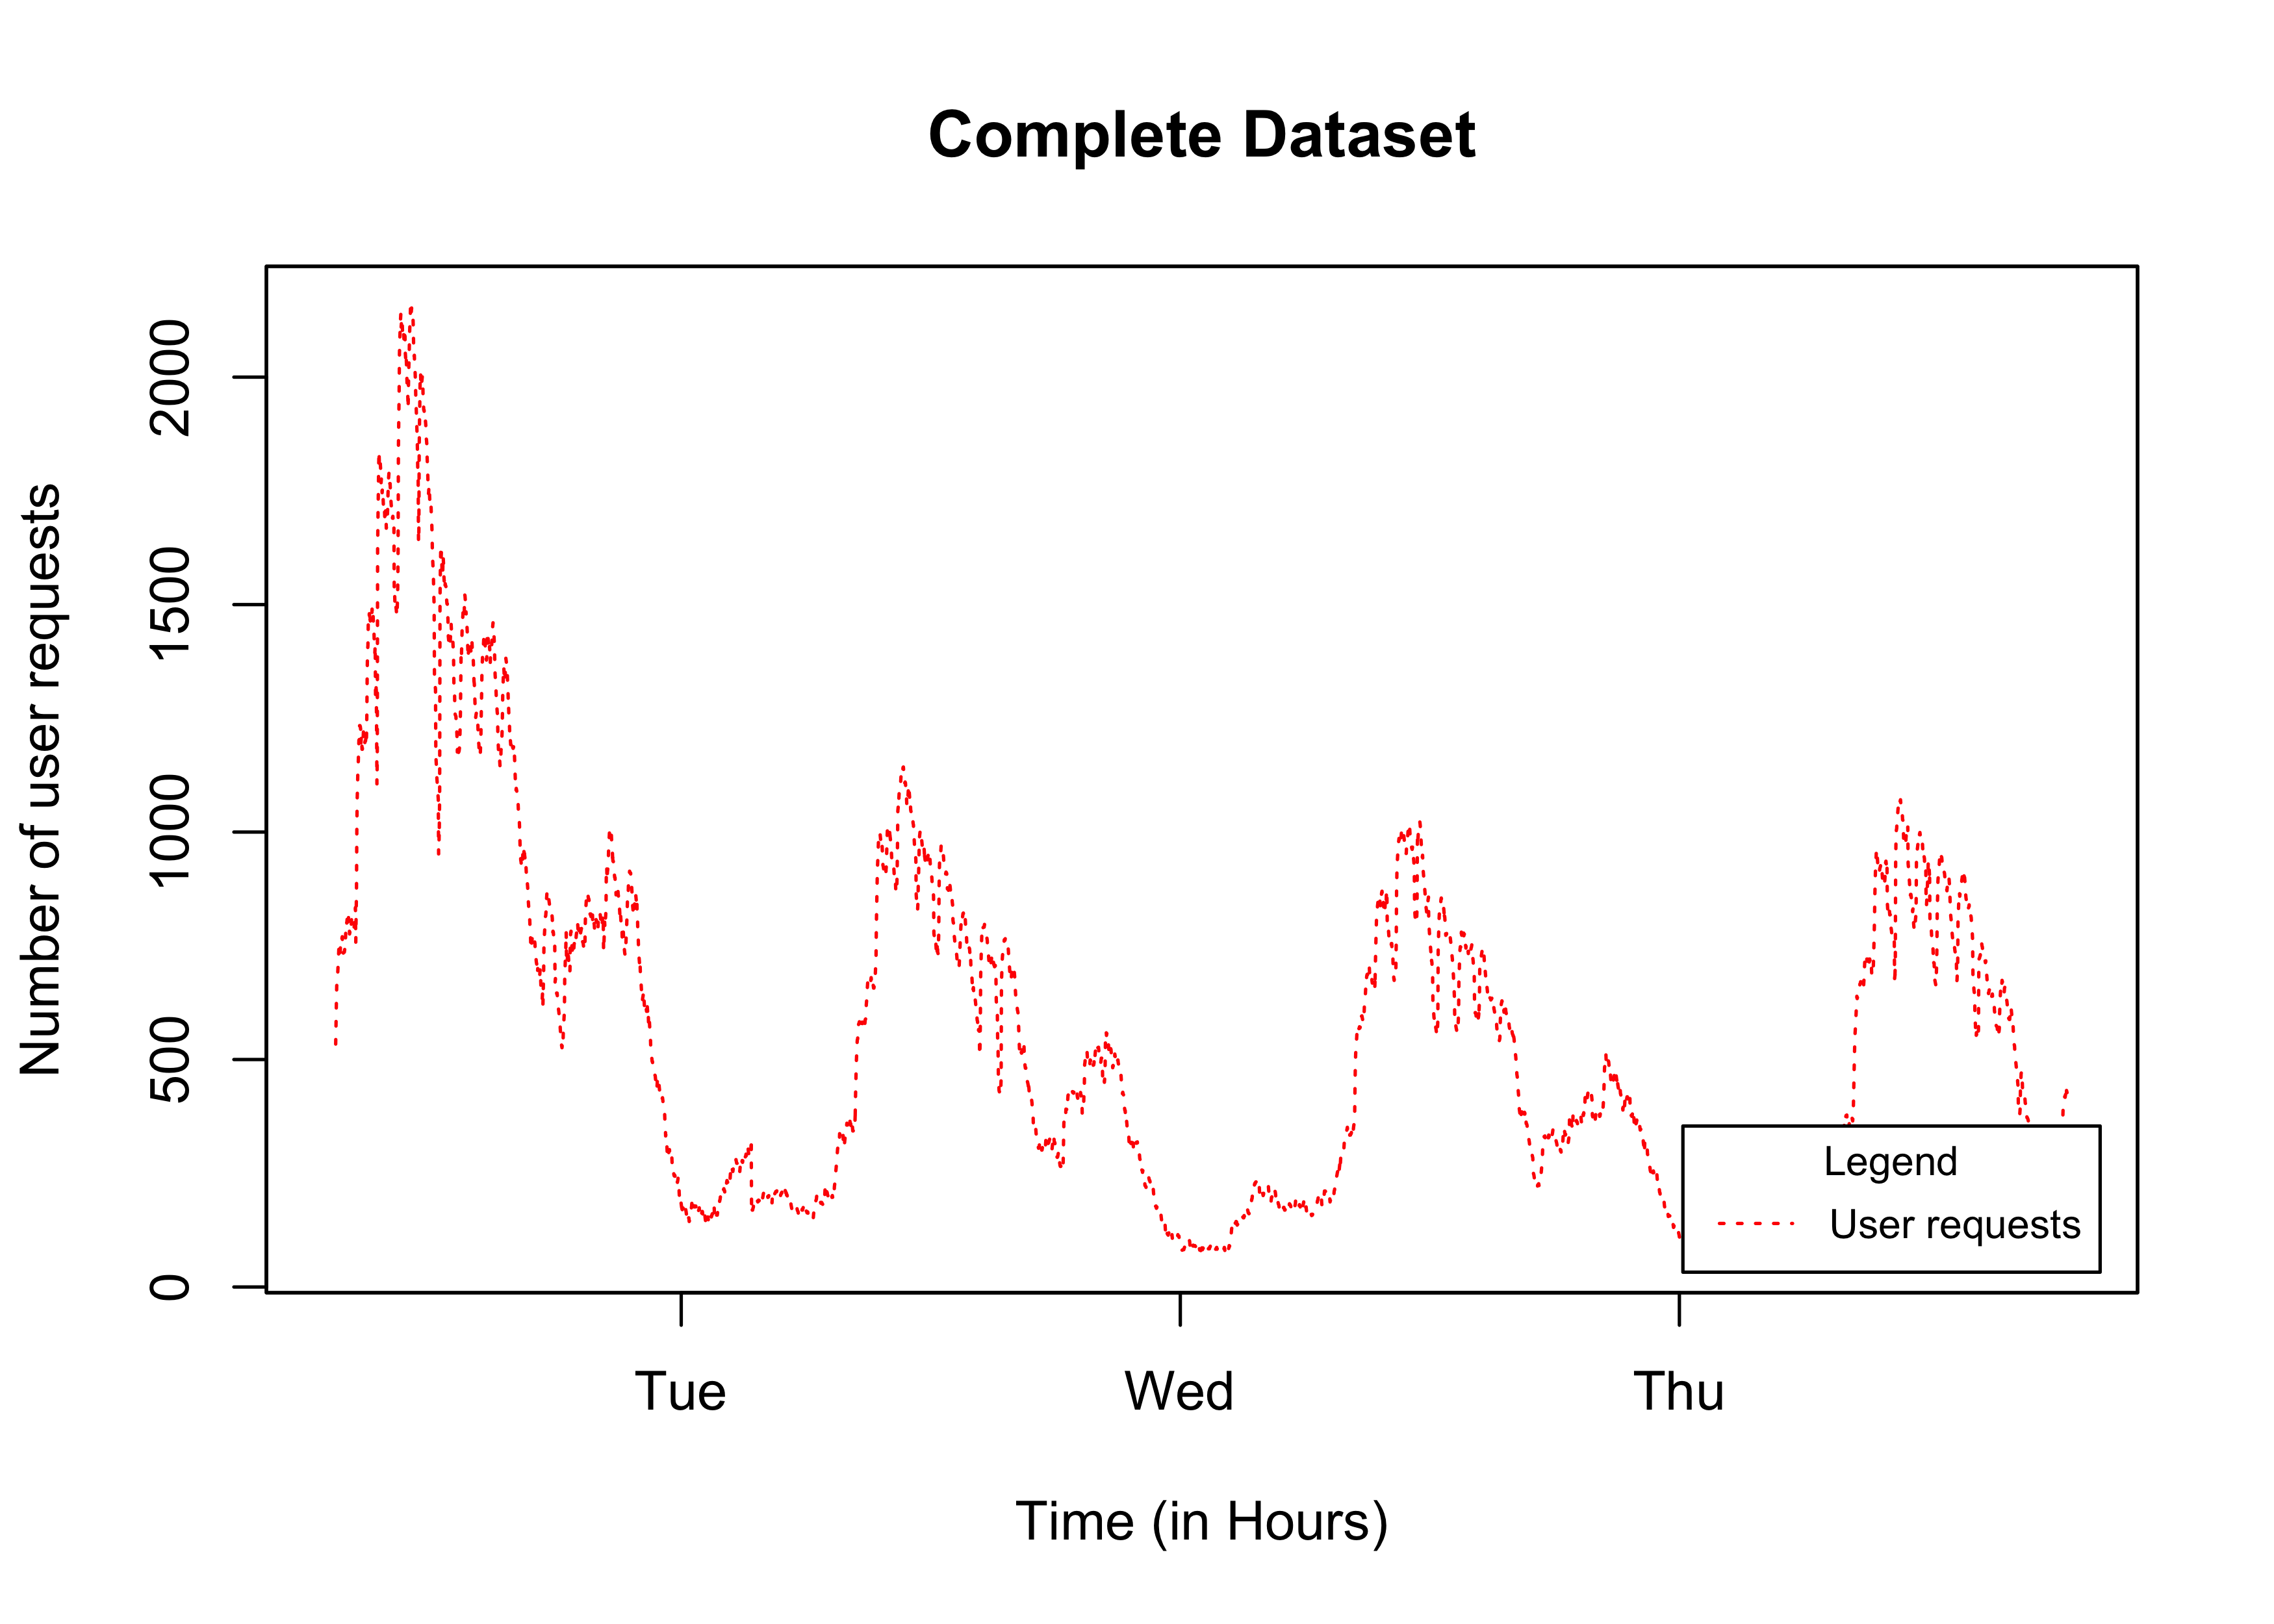
\includegraphics[width=\textwidth]{CompleteWorkload.png}
         \caption{Complete dataset}
         \label{figure:sampleworkload}
     \end{subfigure}
     \begin{subfigure}[b]{0.7\textwidth}
         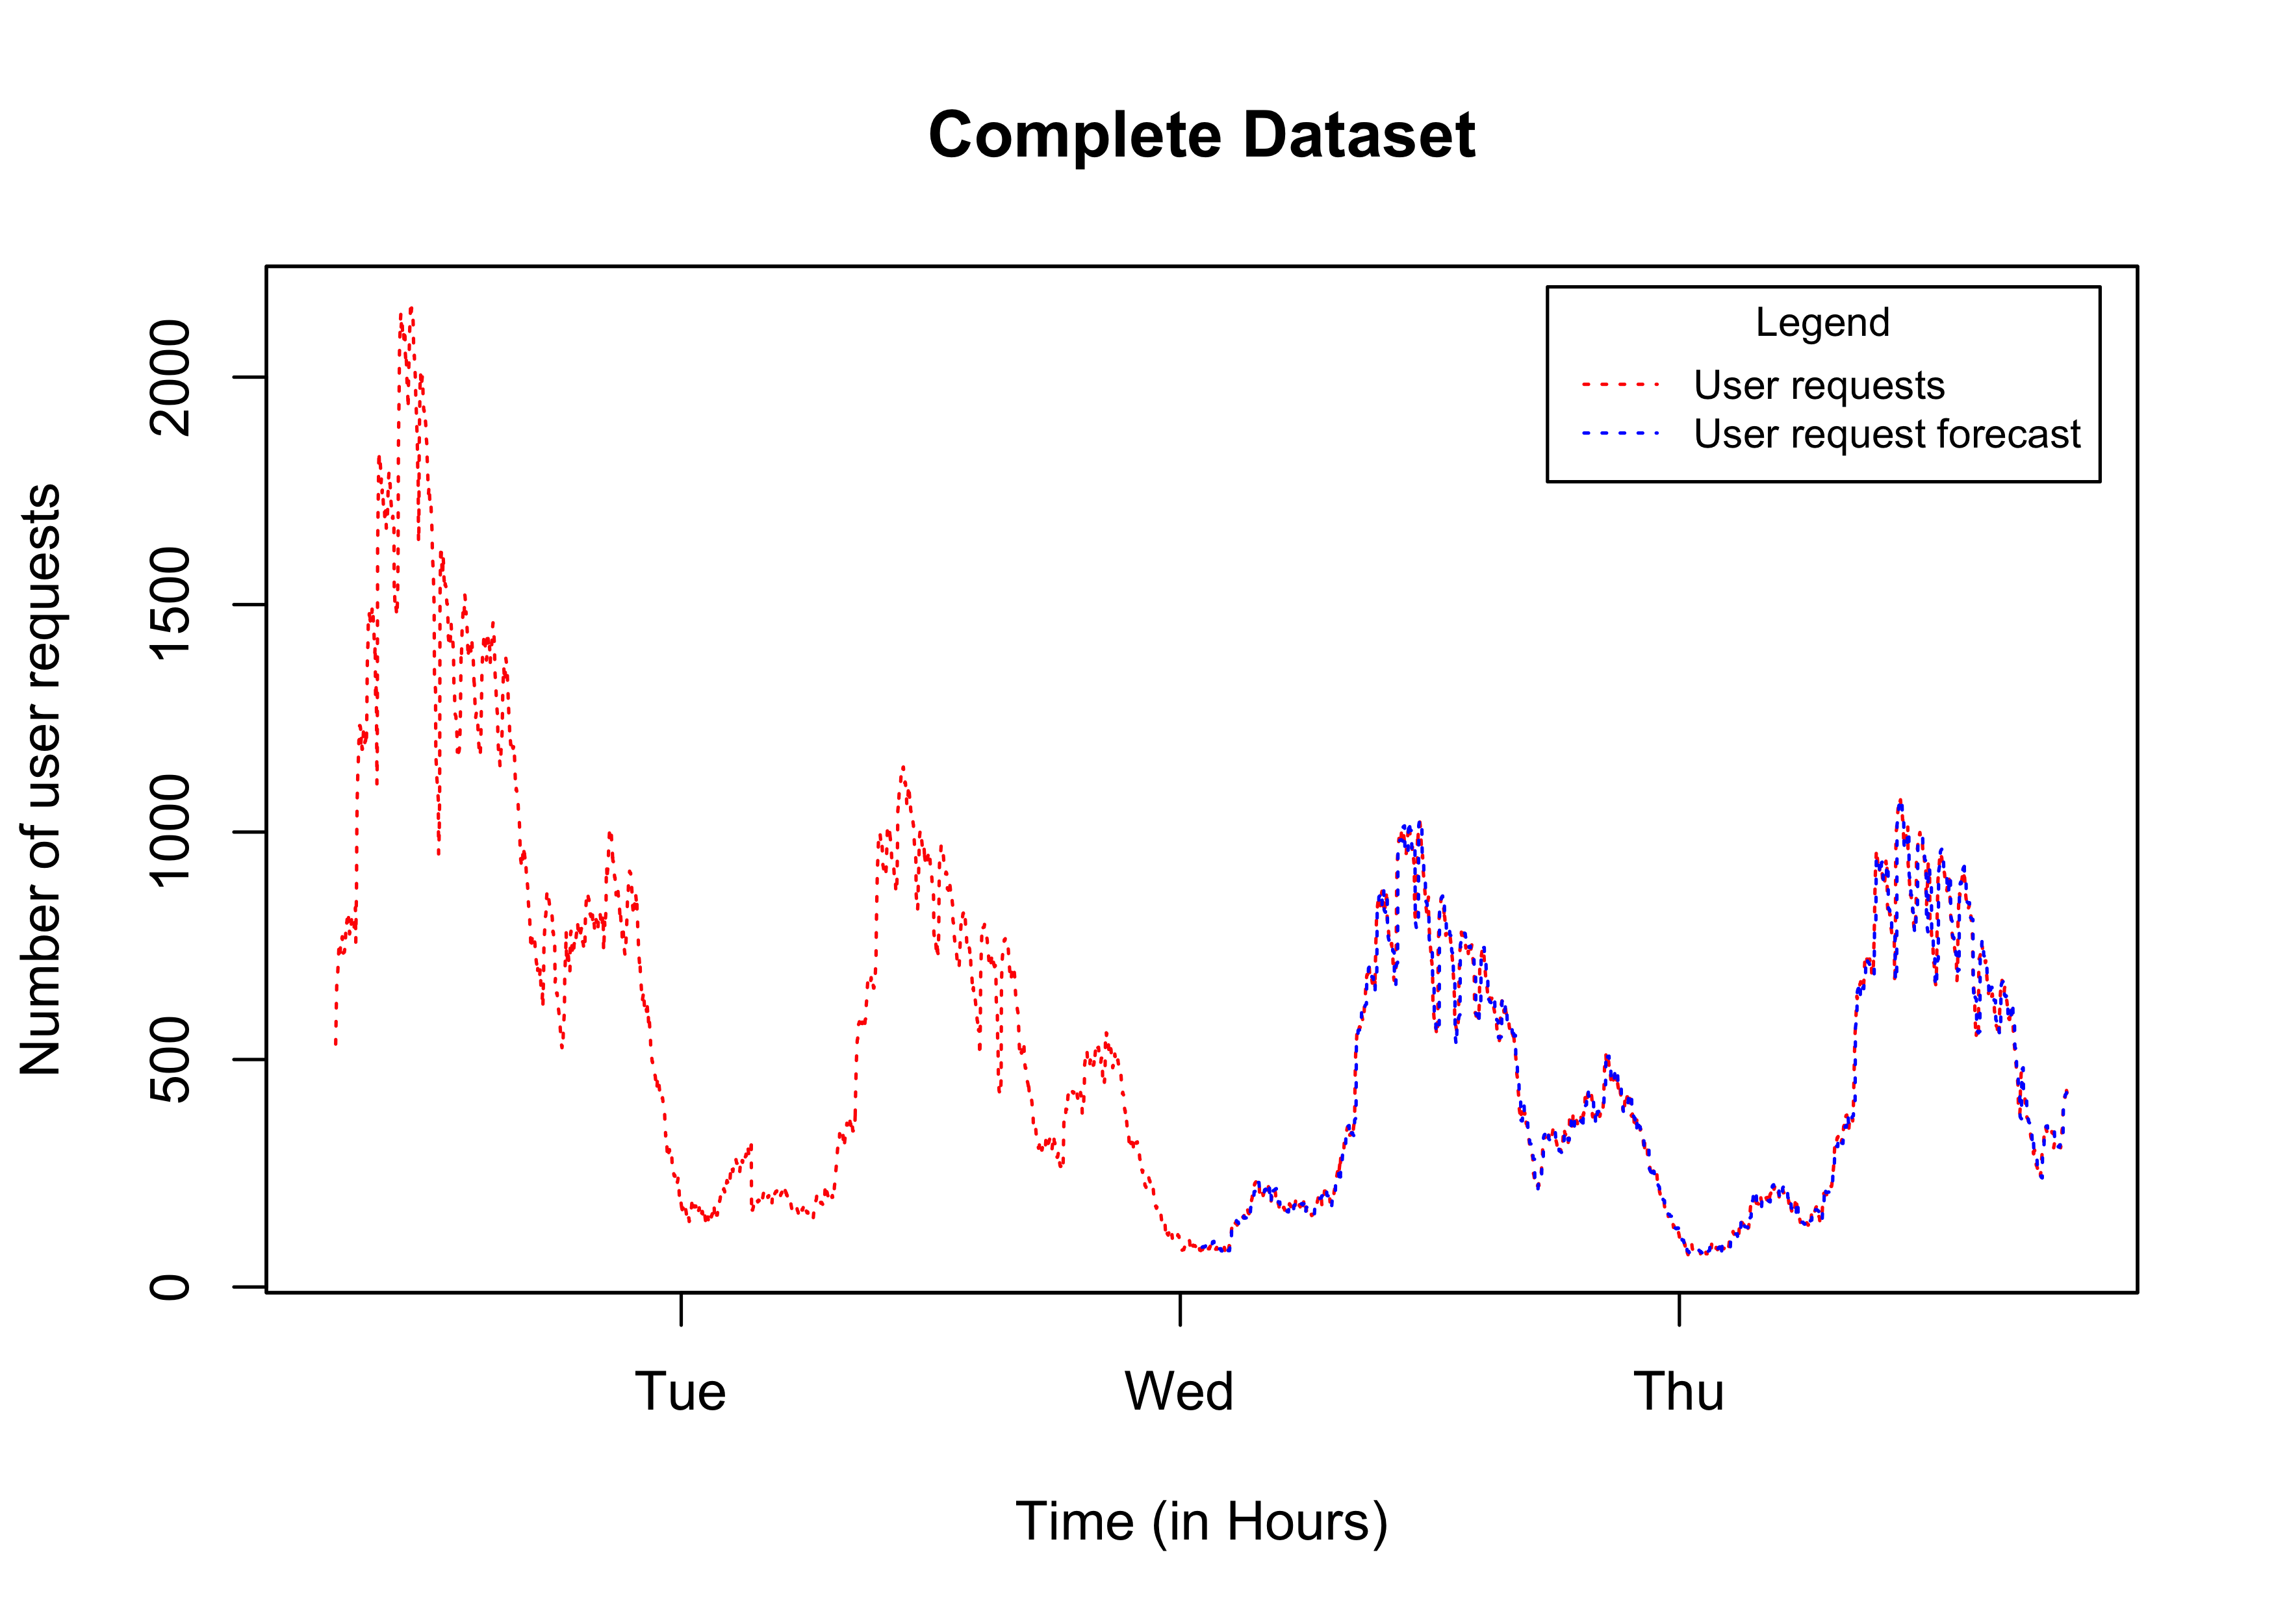
\includegraphics[width=\textwidth]{CompleteWithForecast.png}
         \caption{Actual and forecast dateset}
         \label{figure:forecasted}
     \end{subfigure}
     \caption{Workload observed and forecasted}
     \label{fig:workloads}
 \end{figure}
 \begin{figure}
      \centering
     \begin{subfigure}[b]{0.6\textwidth}
         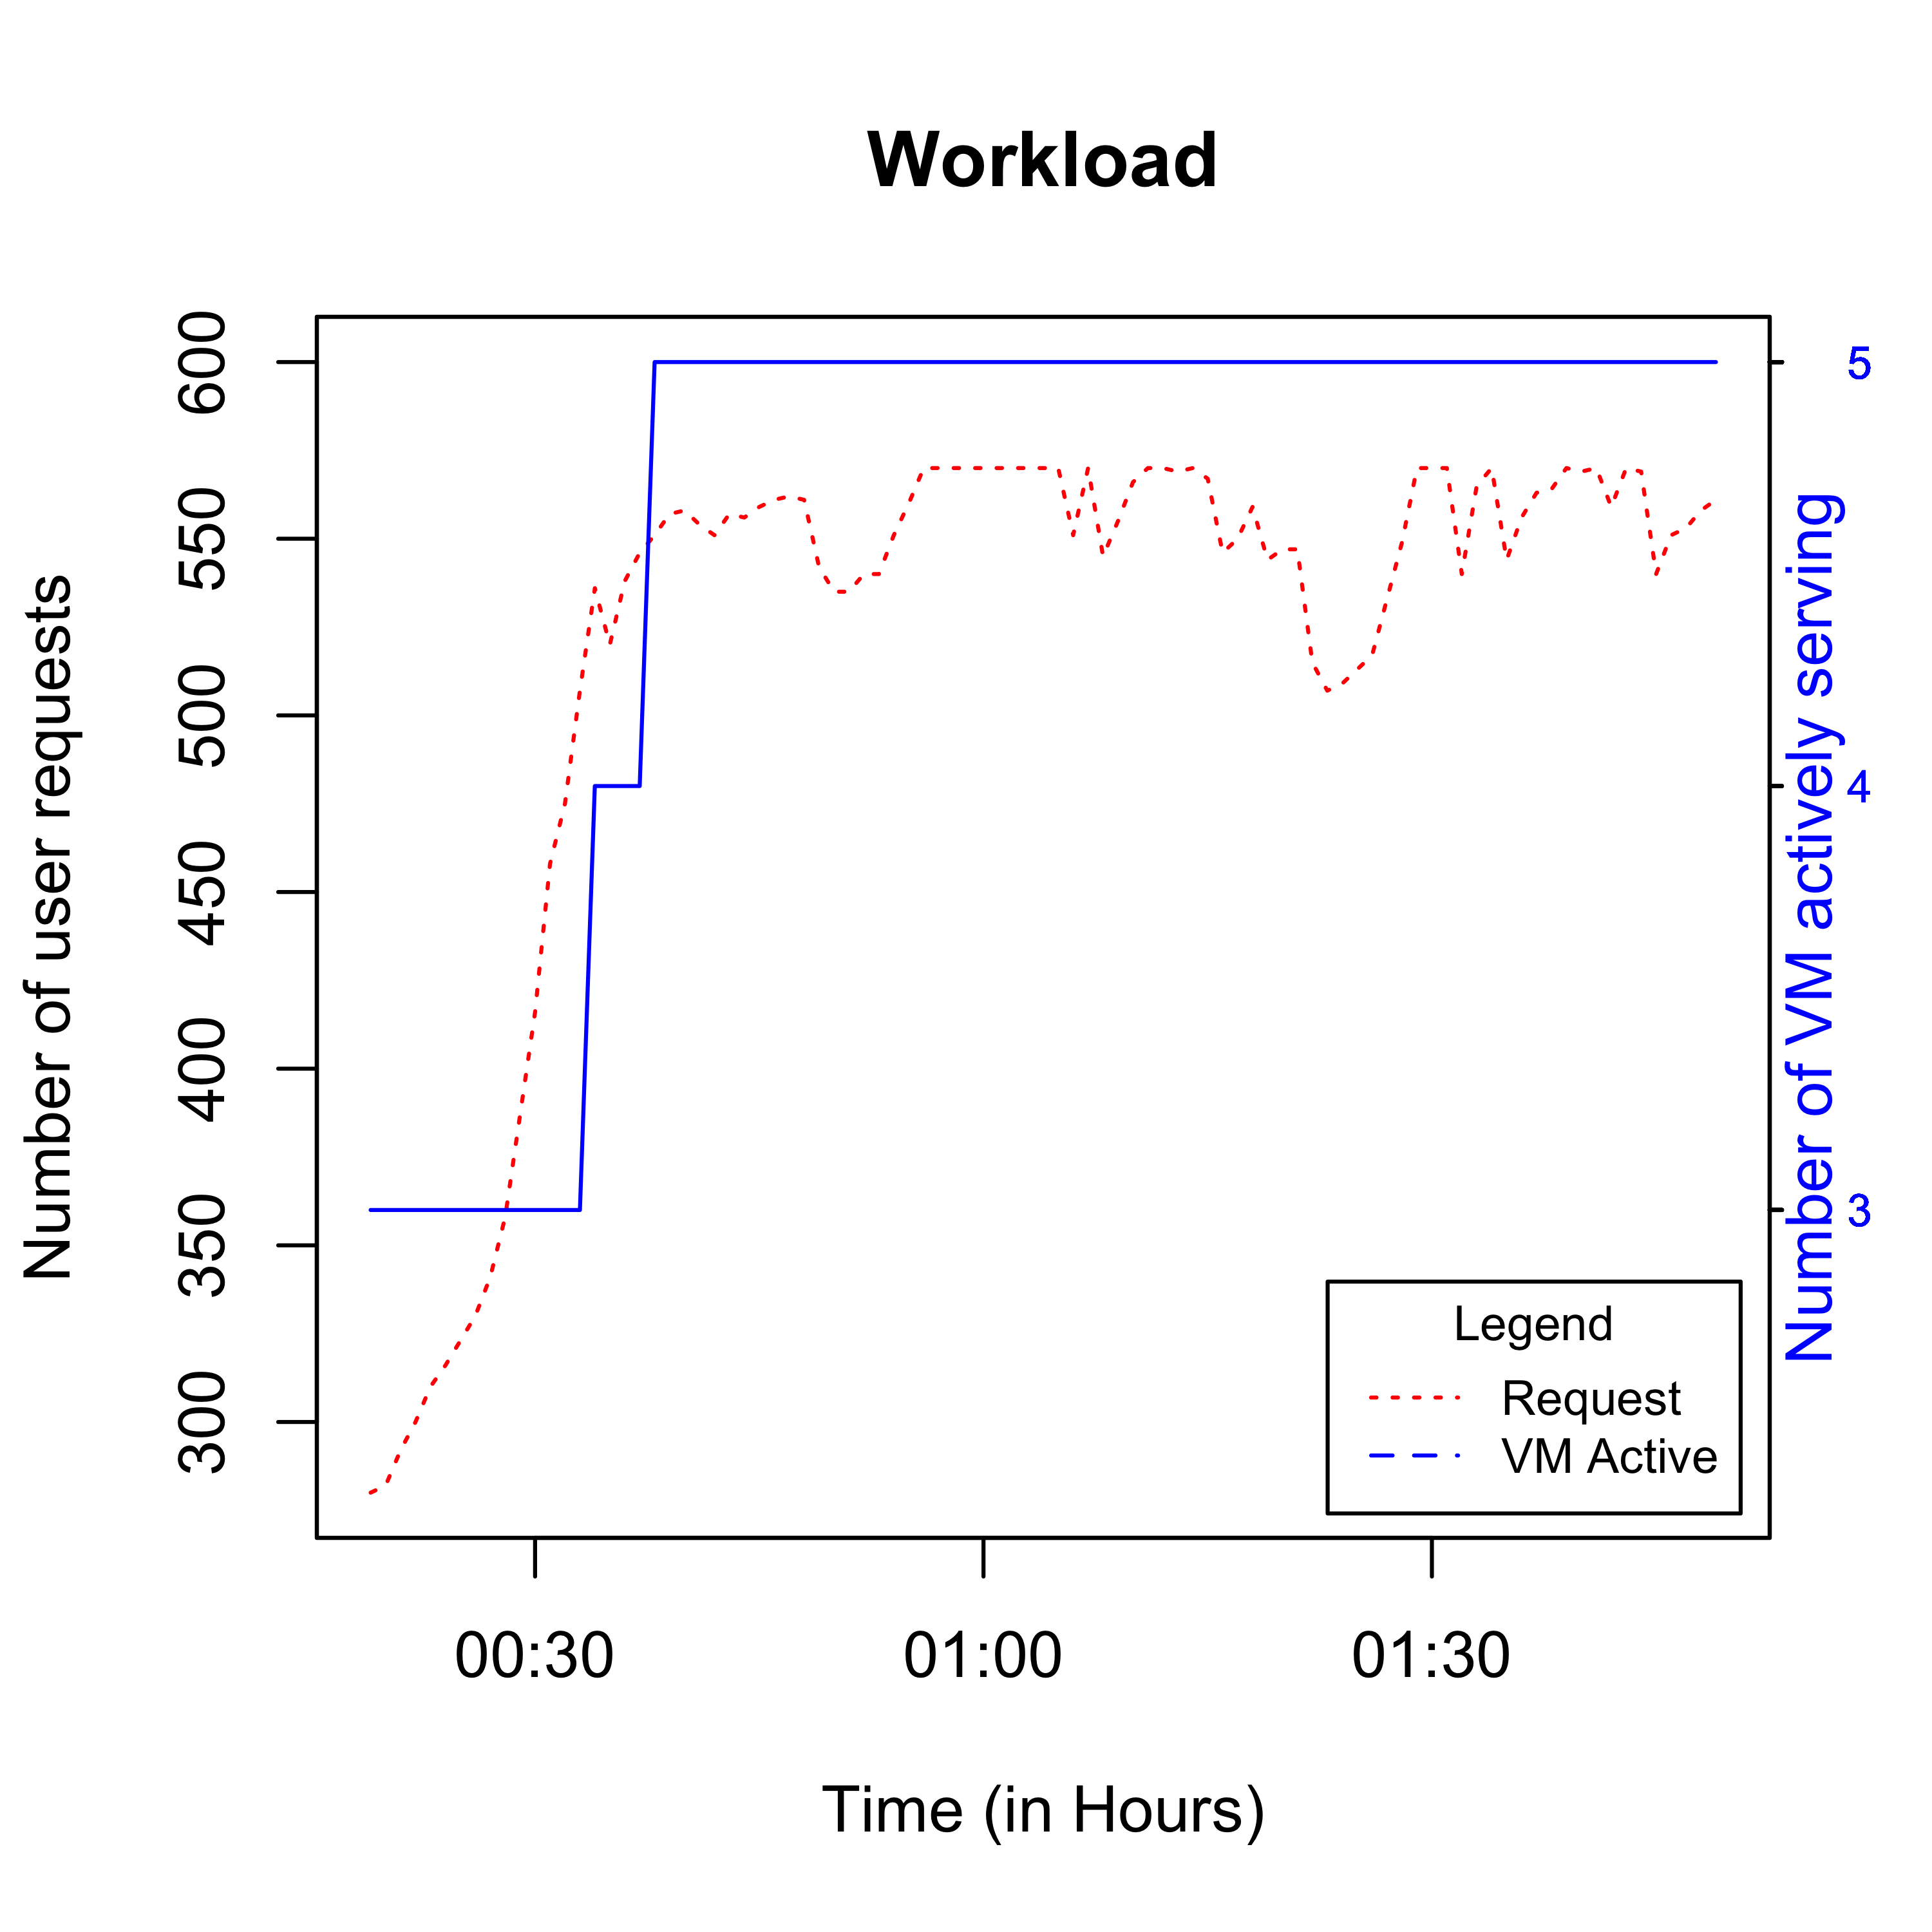
\includegraphics[width=\textwidth]{slaviolationfront.png}
         \caption{SLA Violation exmaple-1}
         \label{figure:slavioa}
     \end{subfigure}
     \begin{subfigure}[b]{0.6\textwidth}
         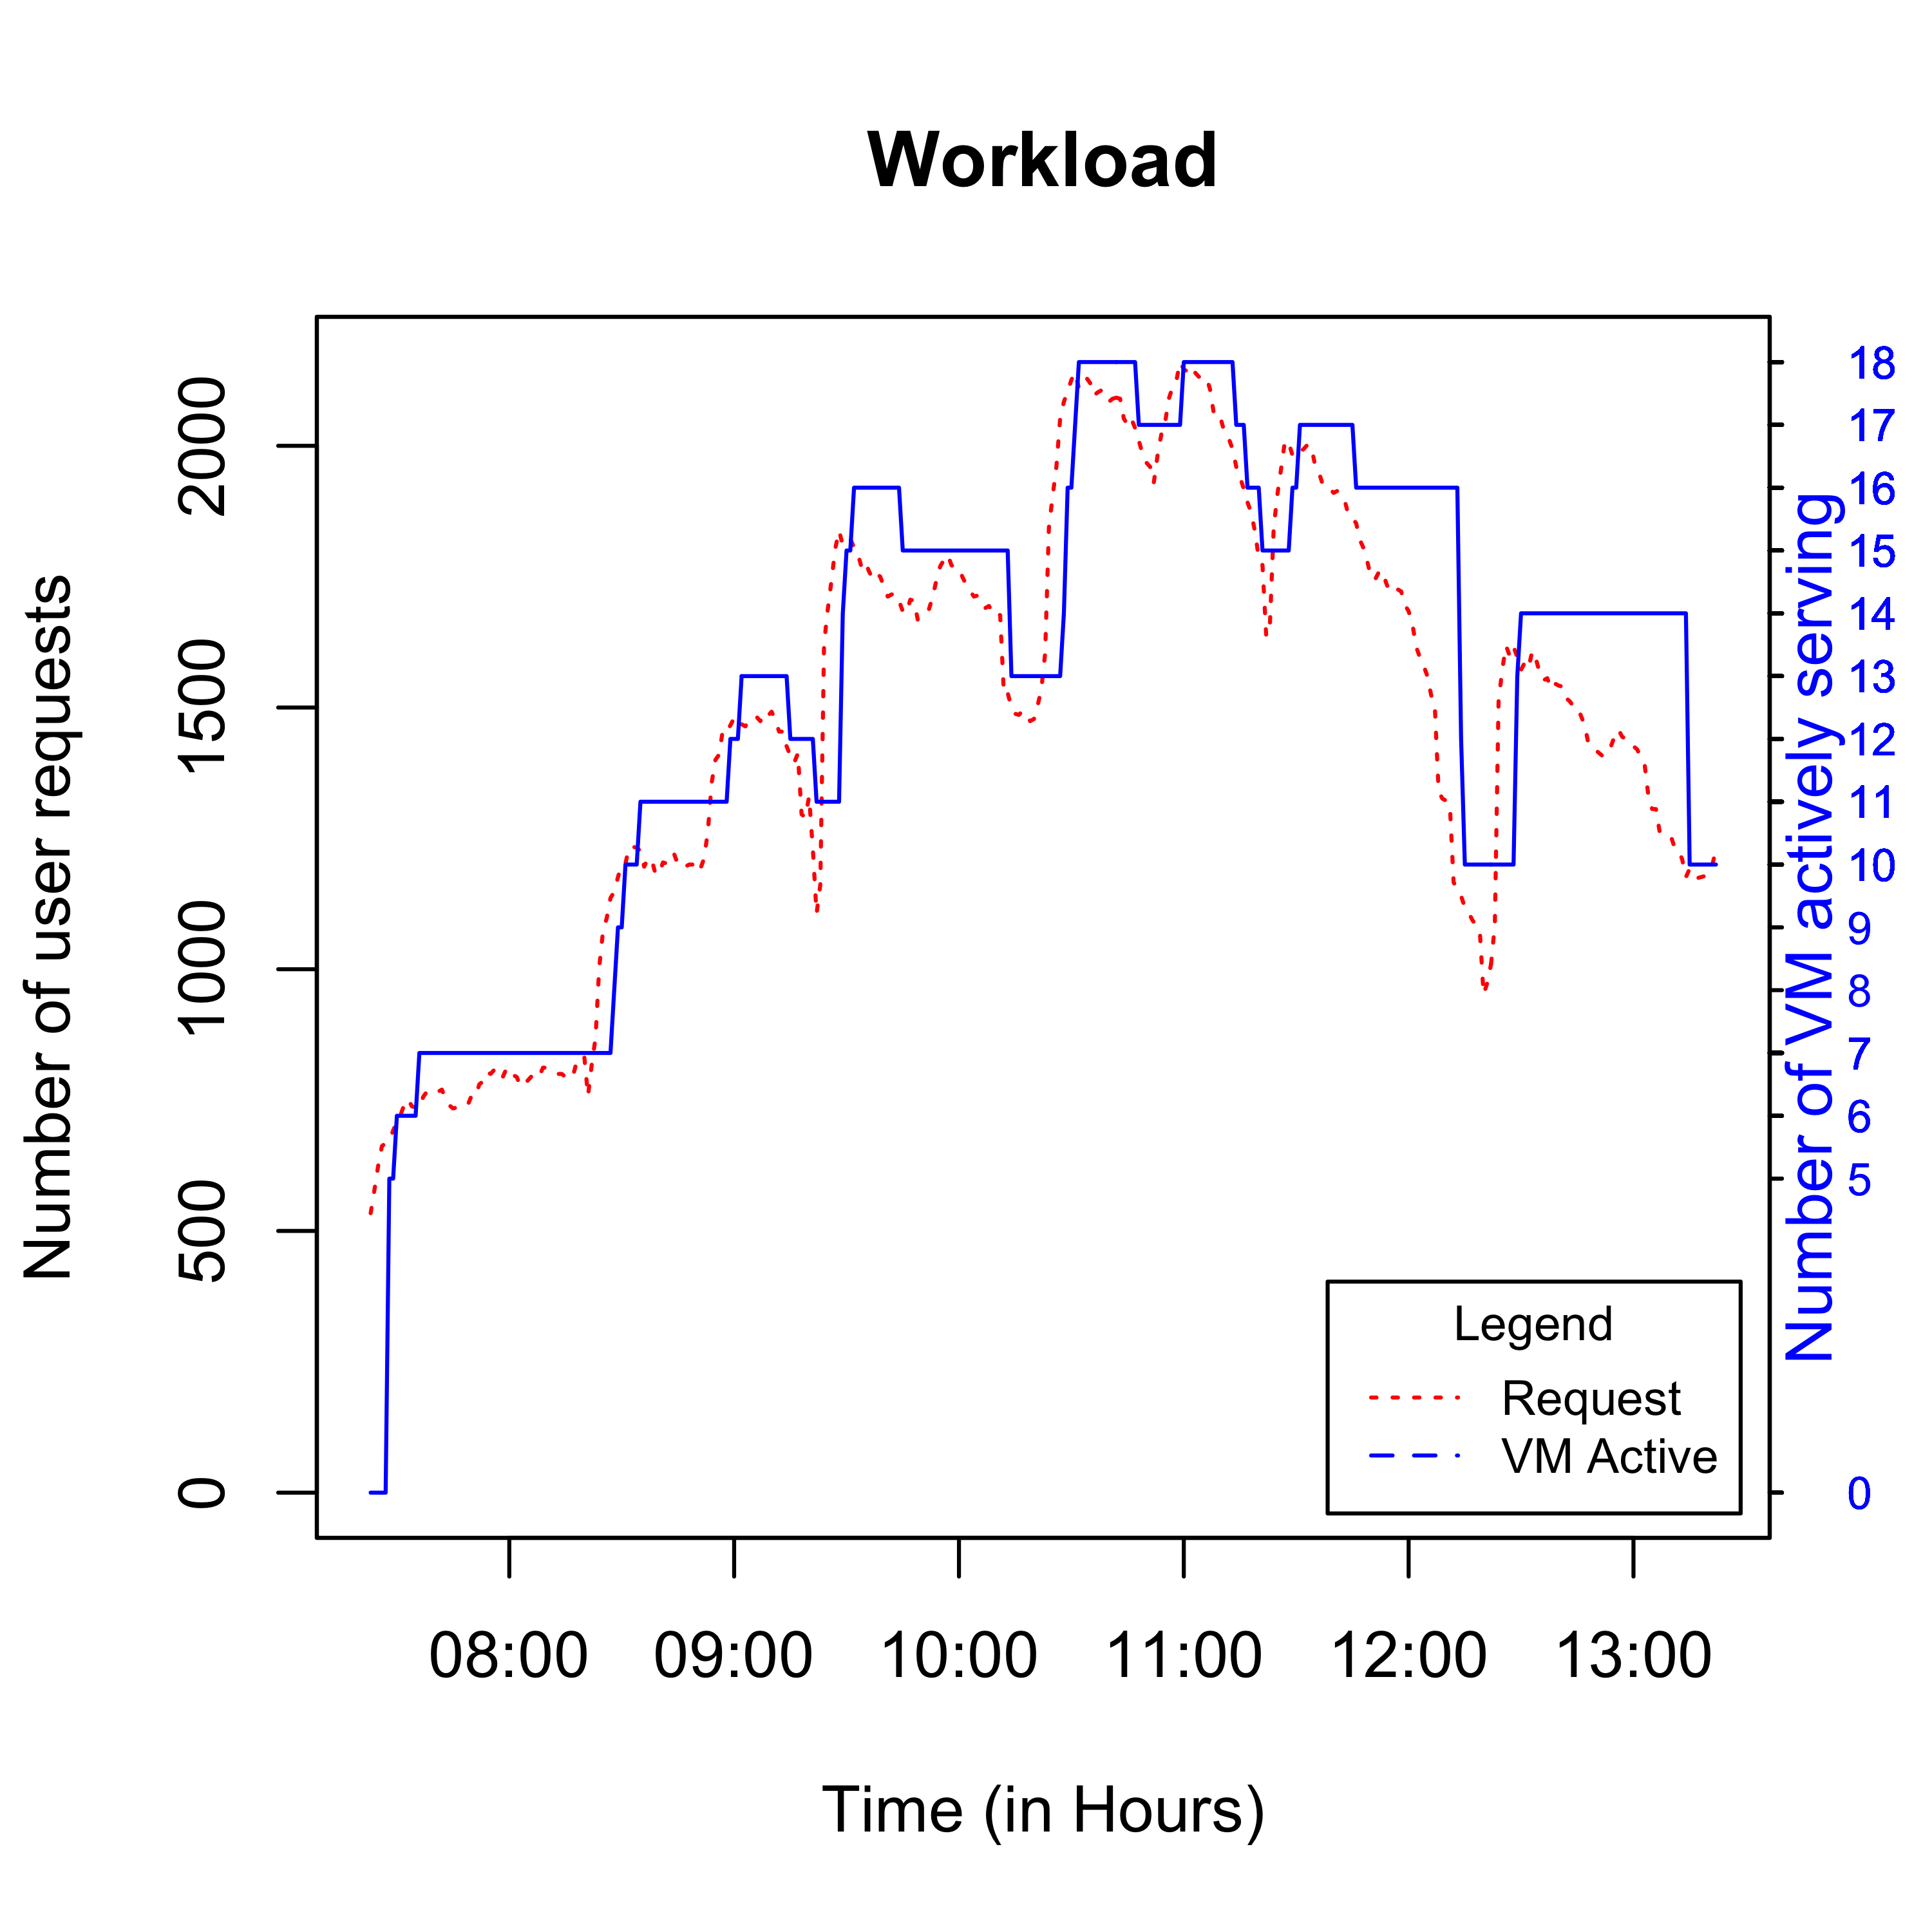
\includegraphics[width=\textwidth]{slaviolationlast.png}
         \caption{SLA Violation exmaple-2}
         \label{figure:slaviob}
     \end{subfigure}
     \caption{SLA violations}
     \label{fig:slaviolationfig}
  \end{figure}


 \section{Simulation design}
 \label{sec:Simulation design}

 \subsection{Design overview}
 \label{sub:Design overview}
 The goal of the simulation is to correctly simulate the behavior of the scaling algorithm in cloud environment from the cloud users perspective. From the cloud users perspective the cloud cost, time to resource allocation, and the VM's utilized are the most important criteria to evaluate cloud service for their cloud hosted application~\cite{kim2015pics}.

 \subsubsection{Key challenges to design ElasticSim}
 \label{subs:Key challenges to design ElasticSim}
 Key challenges faced while designing ElasticSim simulator are:

 \begin{enumerate}
   \item How to model the VM without relaying on any virtualization technologies?
   \item How to handle the user requests data to provide input to the simulator?
   \item How to model the scaling algorithm within the simulator?
 \end{enumerate}

 To solve the first challenge, ElasticSim simulator is designed to model each VM as an object. Simulator user can define diverse VM configurations and its associated cost in a configuration file. For second challenge, ElasticSim provides a data cleaning interface to clean raw data containing user requests to make it efficiently processed by the simulator. Last, to include scaling algorithm the simulator is designed such that the scaling algorithm can be easily interchanged.

 \subsubsection{Simulation Internals}
 \label{subs:Simulation Internals}
 ElasticSim is composed of three layers: Simulation configuration, Prediction and Simulation Core. Figure~\ref{figure:elasticsim} shows all the components of ElasticSim. The simulation configuration layer is responsible for accepting simulation user configurations. The workload prediction layer is responsible for generate prediction based on the specified workloads. The simulation core layer is responsible for including scaling algorithm and also responsible for providing simulation reports. Following is the detailed description about all these layers:
 \begin{itemize}
 \item Configuration Layer: Configuration layer include configuration files to configure various parameter to the algorithm such VM startup time and shutdown, instance cost, billing hour, workloads, number of user per instances as threshold, and  log files. This configuration is designed to simulate various startup/shutdown times, thresholds, workloads and cost. The workload configuration contains detailed configuration of actual and predicted workloads.
 \item Prediction Layer: The simulation prediction layer is responsible for generating the prediction based on ARIMA model and provides two output files, one for scaleup prediction workload and other are scale down prediction.
 \item Simulation Core: Simulation core is responsible for processing the workload events and invoke the scaling algorithm.
 Different components of Simulation core is as show in Figure~\ref{figure:elasticsim}. The Log parser and converter component handles workloads and cleaning the raw data so that its efficient for event processor. Simulation event processor will read each event in workload and invoke scaling algorithm. Scaling algorithm will see the workload and create/release VM instances object represented by VM component. After the scaling algorithm finishes, simulation event processor will invoke the report generator to record the logs and generate the graphs.
 \end{itemize}
 \begin{figure}[h]
   \begin{center}
     \includegraphics[scale=0.6]{ElasticSim.png}
     \caption{ElasticSim System Design}
     \label{figure:elasticsim}
   \end{center}
 \end{figure}

 \RestyleAlgo{boxruled}
 \LinesNumbered
 \begin{algorithm}[H]
  \KwIn{\( U_{i} \),\( B_{p} \),\( T_{start} \),\( T_{shutdown} \), \( Lookahead_{scaleup} \), \( Lookahead_{scaledown}\)}
  \KwOut{Total hours VM instances used, cost of each VM instace.}
  \While{until application is active}{
   \tcc{Get perdicted user request \( r_{i} \) in the time interval \(Lookahead_{scaleup} \)}
   \(r_{i}\) = \(max\)(getPredictedUserRequest(\(Lookahead_{scaleup}\)))\;
   \tcc{new machines \( n_{i} \) required in the interval \(Lookahead_{scaleup}\)}
   \( n_{i} = r_{i} / U_{i} \)\;
   \tcc{machines already running \( m_{i} \) at time \( t_{i} \)}
   \( m_{i} = getRunningVmInstanceCount() \)\;
   \uIf{\( n_{i} > m_{i} \)}{
     \tcc{Add more machines}
     \(newMachinesToStart =  n_{i} - m_{i}\)\;
     \lFor{ i=1 \emph{\KwTo} newMachinesToStart }{
     \tcc{New VM takes \( T_{start}\) mins to start}
     start new VM instance
     }
    }
    \uElseIf{\( n_{i} < m_{i} \)}{
    \tcc{Get predicted user request \( r_{i} \) in the time interval \(Lookahead_{scaledown}\) to check if machines can be extended billing period}
    \(r_{i}\) = \(max\)(getPredictedUserRequest(\(Lookahead_{scaledown}\)))\;
    \( n_{i} = r_{i} / U_{i} \)\;
    \(machinesToShutdown =  m_{i} - n_{i}\)\;
     \tcc{Stop machine before billing period to avoid billing to next hour since machines take \( T_{shutdown}\) mins to shutdown. Only stop machines which are nearing billing period.}
     \lFor{ i=1 \emph{\KwTo} machinesToShutdown }{ Stop VM instance ending billing period }
   }
  }
  \caption{AppElastic Algorithm with look-ahead}
  \label{algo:appelasticwithlookahead}
 \end{algorithm}

 \section{Summary}
 \label{sec:Summary}
  Section~\ref{sec:AppElastic Algorithm} introduced and explain AppElastic algorithm. At first AppElastic was discussed without the capability of workload forecasting. Then the drawbacks of this approach was solved after introducing ARIMA time series forecast model. AppElastic algorithm was extended with lookahead feature so that it can provision the VM's before hand.

 In Section~\ref{sec:Simulation design} to test the algorithm in a simulation environment ElasticSim simulator design was introduced. Here  the concepts and ideas of simulator was introduced and explained. It also introduced how ElasticSim helps modeling cloud environment without having to interact with cloud service provider or virtualization technologies.


\chapter{Implementation and Evaluation}
\label{chap:ImplementationEvaluation}
In this chapter the implementation details are introduced and the evaluation of the AppElastic algorithm combined with workload forecasting is presented. This chapter start with presentation of simulator called ElasticSim. Then details about the implementation of forecast algorithm is presented. In Section~\ref{sec:AppElastic Algorithm Implementation}, details about the implementation of AppElastic algorithm is explained with few code snippets. In the later sections of this chapter accuracy of the forecast model is discussed and the effectiveness of the AppElastic algorithm is presented.

\section{ElasticSim}
\label{section:ElasticSim}
Design of the ElasticSim was introduced in previous chapter and its three layers: Configuration, Prediction and Simulation Core layers, were presented. The implementation details of ElasticSim is discussed in this section.

\subsubsection{Technology Selection}
\label{subs:Technology Selection}
ElasticSim is composited of various technologies. The configuration layer and simulation core is implemented in Java\footnote{http://java.net/}. Where as the prediction layer is implemented in R scripting language\cite{rstat}. These two layer are interconnect with Bash scripting\footnote{https://www.gnu.org/software/bash/}.

\subsubsection{ElasticSim Operation}
\label{subs:ElasticSim Operation}
ElasticSim at a high level provides four different operations. These operations are provided at the start of the simulator. The start screen of the simulator is as shown in the Figure~\ref{figure:simwelcome}. These options serves four different functionality, this is as described below:

\begin{enumerate}
  \item First option consist of R scripts which implements the workload forecast functionality. The prediction script reads the workload trace file, split the input into two half, for testing and training, and runs ARIMA forecast model.
  \item Second option runs the AppElastic algorithm on historical workload traces, so that the simulation users can decide on number of reserved instances to choose for reservation.
  \item Third options runs the AppElastic algorithm on a given workload trace and considers different instance types. Here the user specify number of reserved instances to use for this simulation run.
  \item Fourth options runs the AppElastic algorithm to generate the simulation logs so that a newly built scaling algorithm can be tested easily.
\end{enumerate}

\begin{figure}[h]
  \begin{center}
    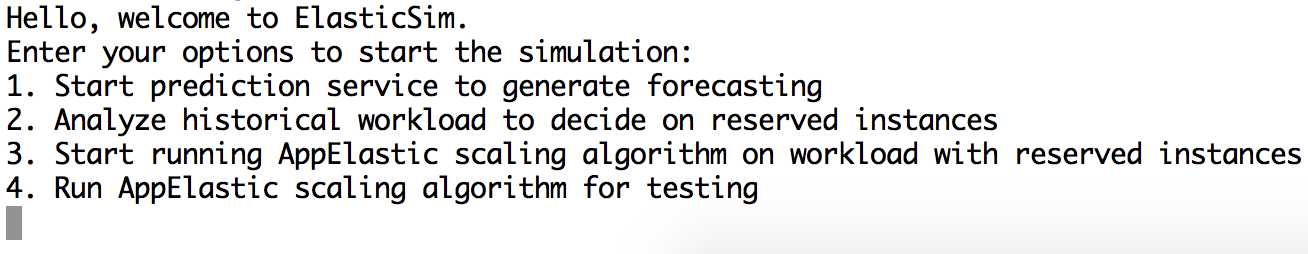
\includegraphics[scale=0.6]{simwelcome.png}
    \caption{ElasticSim}
    \label{figure:simwelcome}
  \end{center}
\end{figure}

\subsubsection{Input to ElasticSim}
\label{subs:Input to ElasticSim}
Inputs to ElasticSim is provided through a simple configuration interface. This simulator configuration file is as show in the Figure~\ref{figure:simconfig}. ElasticSim uses these configuration values for providing input to the algorithm. These configurations can be grouped into five types: VM configuration, AppElastic configuration, Cloud service provider related configuration, Workload trace configuration, Output log configuration. These types can be explained as follows:

\begin{itemize}
  \item VM configuration include VM startup and shutdown time. These time is configured through the variable VM\_START\_TIME and VM\_SHUTDOWN\_TIME respectively.
  \item Since AppElastic is a threshold based algorithm. Threshold can be easily configured by assigning values to NUMBER\_OF\_USERS\_PER\_INSTANCES variable. Lookahead period for AppElastic can be configured through LOOKAHEAD\_SCALEUP and LOOKAHEAD\_SCALEDOWN variables.
  \item Cloud service provider related configuration includes instance purchasing, billing period. To configure different instance pricing variables like COST\_RI and COST\_ODI are supported. Billing period according to cloud service provider is configured through the variable BILLING\_PERIOD.
  \item Workload trace configuration includes training and testing workload traces. Variable ACTUAL\_WORKLOAD is used to configure testing workload trace. The predicted workload traces from forecast model will produce two log traces for scale up and scale down, and these log traces are configured through variables FORECAST\_SCALEUP\_WORKLOAD and FORECAST\_SCALEDOWN\_WORKLOAD, respectively.
  \item Output from the ElasticSim will be recorded into files. To configure the file name for simulation output, SYSTEM\_LOG variable is assigned a valid file name on the local disk.
\end{itemize}
The simulator user can use their algorithm by replacing the implementation of the algorithm. The simulator users are able to leverage this mechanisms to design and test their own scaling algorithm.
\begin{figure}[h]
  \begin{center}
    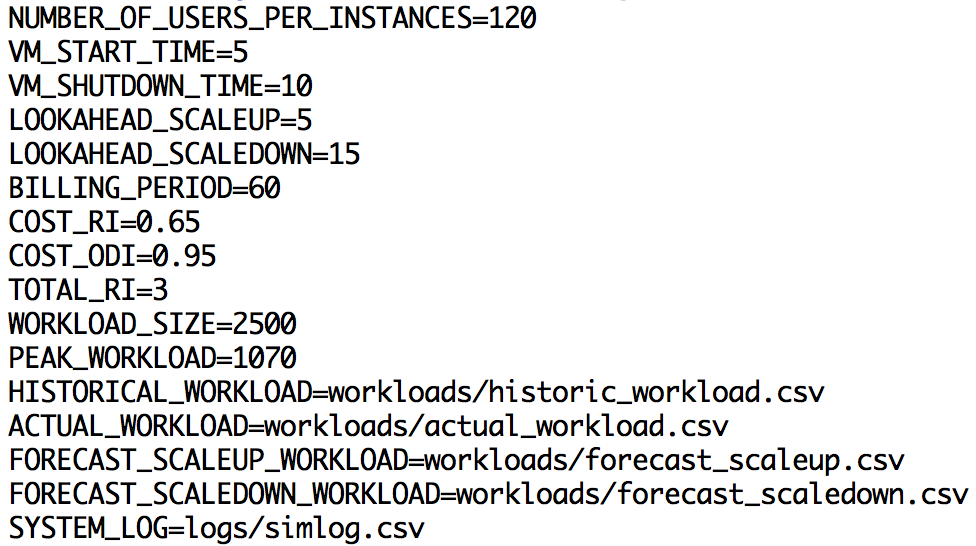
\includegraphics[scale=0.7]{simconfig.png}
    \caption{Simulation Configuration}
    \label{figure:simconfig}
  \end{center}
\end{figure}

\subsubsection{Output from ElasicSim}
\label{subs:Output from ElasicSim}
ElasicSim outputs are provided through logs and reports. Details of the logs generated, as comma separated value(csv), after each simulation run is provided here and the reports as output are discussed in evaluation section. ElasticSim provides two types of log files as output: VM usage logs and AppElastic logs. These two logs are as shown in the Figure~\ref{fig:elasticsimlogs}. These output is detailed as follows:
\begin{itemize}
  \item As shown in the Figure~\ref{figure:costlog}, VM usage log provides details about VM based on VM-ID. Billing hour start and Billing hour end fields are provided to identify the billing period of each VM. VM activity start and VM activity end fields are used to find in what period the VM was actively serving users. These time are recorded as Unix timestamps. VM usage time is recorded in Usage (in Minutes) field and the cost of using VM based the billing hours is recorded in Cost field.
  \item In Figure~\ref{figure:appelasticlogs}, logs related to AppElastic algorithm is shown. Its important to identify any anomaly in scaling algorithm, hence ElasticSim provides a detailed log of scaling. Logs are recorded for each time interval and helps in identifying the actual number of user request, number of VM's needed to serve these users and VM's provided by AppElastic algorithm. Each time interval is represented as unix timestamp in the field Unix timestamp. Actual number of users in the system is recorded in the field User request. Based on the threshold specified in the configuration and for the current number of user requests, VM required is recorded in VM needed field. VM activity such as billing start and activity start time are recorded VM active and VM billing fields respectively.
\end{itemize}
\begin{figure}
     \centering
     \begin{subfigure}[b]{1.0\textwidth}
         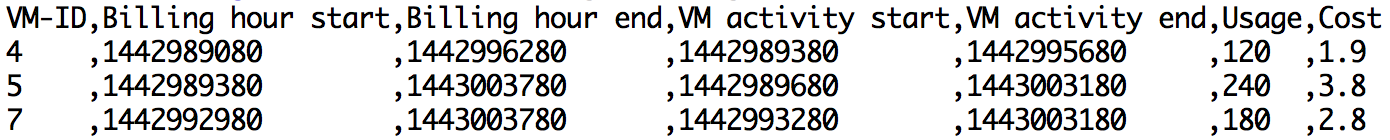
\includegraphics[width=\textwidth]{billinglog.png}
         \caption{VM usage log}
         \label{figure:costlog}
     \end{subfigure}
     \begin{subfigure}[b]{0.9\textwidth}
         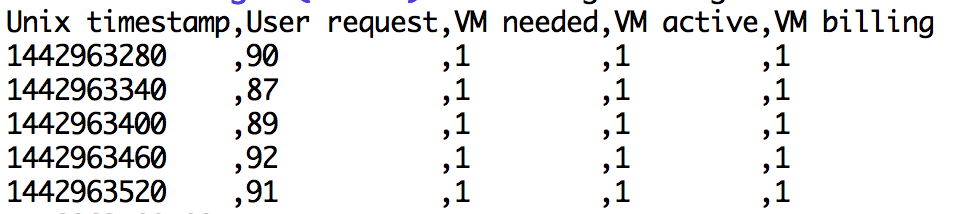
\includegraphics[width=\textwidth]{simlog.png}
         \caption{AppElastic logs}
         \label{figure:appelasticlogs}
     \end{subfigure}
     \caption{Output log from ElasticSim}
     \label{fig:elasticsimlogs}
 \end{figure}
 \section{Modeling workload \& prediction}
\label{sec:implementationprediction}
In this section implementation details of workload prediction is presented. ARIMA model discussed in the earlier chapter is applied to workload log trace and used for forecasting. Common obstacle for many while developing ARIMA model for forecasting is the selection of order of ARIMA process which considered as subjective and difficult task~\cite{makridakis2008forecasting}. Many years of research has gone into developing an automated approach to ARIMA model building. As introduced in the related work chapter, model building for ARIMA(p,d,q) process requires to choose values for p,d and q. Manual selection of these parameter works if the input time series is know prior to building time series model. Since, the workload arriving to the system cannot be modeled easily there is a need for automating the model building. Solution to automated ARIMA model selection process is given by Hyndman et al.\cite{hyndman2007automatic}. The algorithm guarantees to halt and return a valid model\cite{hyndman2007automatic}. This selected model is used for forecasting. The algorithm by Hyndman et al\cite{hyndman2007automatic} is implemented in a package called \(forecast\) in R software~\cite{rstat}. The implementation details of \(forecast\) library  and \(auto.arima()\) method are out of scope of this thesis. The function \(auto.arima()\) is used as black-box because the mechanism that transform the input workload into output model is obfuscated and out of scope of this thesis. A code snippet of forecasting workload for scale up is given in Listing~\ref{list:predscaleup}. For workload modeling reads the csv input workload trace and converts it into input time series data using R library called \(zoo\). In line number 5 and 6, the input timeseries data is divided into two parts. One for training and other for testing the model. The forecasted values are stored in \(arimaScaleupPrediction\) vector. The for loop in line 11 goes through the workload time series and starts building ARIMA model with the help of \(auto.arima()\) function. Since the training and testing datasets are on the same time scale, the for loop start from training dataset and runs until the end of the testing data each time including observed data from test for every forecast interval. On the first iteration, first part of the workload i.e the training dataset is included into the model. On each iteration of the loop, new data points in the test dataset is included along with training data. Model building and forecasting is repeated every forecast interval as specified in forecast\_interval parameter. Actual forecasting of the data points is done in the line number 13. Forecasting is done with the help of a function called \(forecast\) and the forecast horizon is specified in horizon\_scaleup for scaleup. The forecast accuracy is recorded after every forecasting, and is recorded to a file as specified in line 14. Code snippet for predicting scale down time series is same as scale up prediction, but the only differing is in the horizon value which will be different.
\begin{lstlisting}[language=R,caption=ARIMA Scaleup Model,label=list:predscaleup,numbers=left,frame=single,fontadjust=true,breaklines,basicstyle=\small]
workload=read.csv(WORKLOAD,sep=",",header=F);
workload_header=c("UnixTimeStamp","ActiveSessions");
colnames(workload) <- workload_header;
workload_tsdata=zoo(workload$ActiveSessions,workload$posxtime);
trainsamples=workloadsize/2;
testsamples=workloadsize/2;
#Forecast interval in minutes
forecast_interval=5;
#predict for scaleup
arimaScaleupPrediction=c();
for (i in seq(trainsamples,workloadsize,forecast_interval)){
  arimaFit=auto.arima(workload_tsdata[1:i])
  pred=forecast(arimaFit,h=horizon_scaleup)
  sink("accuracy_scaleup.log",append =T);
  print(accuracy(pred));
  sink();
  arimaScaleupPrediction=c(arimaScaleupPrediction,pred$mean);
}
\end{lstlisting}
Numerous error metrics have been proposed to capture the different between point forecast and corresponding observations. One of the most common forecast accuracy metric is based on mean square error (MSE)\cite{makridakis2008forecasting}. MSE is classified as scale dependent error metric. In the scope of this thesis, mean absolute percentage error (MAPE)\cite{makridakis2008forecasting}, which is a measure of prediction accuracy of forecasting model. MAPE is given by the formula:
\begin{equation}
  MAPE = 1/n \sum_{t=1}^{n} |\frac{A_{t}-F_{t}}{A_{t}}|
\end{equation}
where \(A_{t}\) is the actual value and \(F_{t}\) is the forecast value. The difference between \(A_{t}\) and \(F_{t}\) is then divided by the Actual value \(A_{t}\). The absolute value in this calculation is summed for every forecasted point in time and divided by the number of fitted points \(n\). Multiplying by 100 makes it a percentage error. Complete details of ARIMA model forecast accuracy is given evaluation section.
\section{AppElastic Algorithm Implementation}
\label{sec:AppElastic Algorithm Implementation}
In order to achieve the main research goal, that is to develop autoscaling algorithm, AppElastic algorithm is implemented in Java programming language. As said earlier AppElastic algorithm is a threshold based algorithm, it consist of three main internal parts as shown in the Figure~\ref{figure:appelasticparts}, and is described as follows:
\begin{itemize}
  \item Reading actual and predicted workloads: ElasticSim will guide the AppElastic algorithm in giving access to the log traces. ElasticSim generates the events for each entry in the log trace, accordingly AppElastic algorithm reads the actual and predicted log traces to apply main algorithm logic.
  \item  Reading scaling thresholds configuration: The threshold information are as part of the ElasticSim configuration. AppElastic algorithm will read this threshold values to make the scaling decision.
  \item Generating scaling action using AppElastic Algorithm: Actual algorithm will run on the input data and generates the scaling actions.
\end{itemize}
\begin{figure}[h]
  \begin{center}
    \includegraphics[scale=0.7]{scaling.png}
    \caption{Parts of AppElastic}
    \label{figure:appelasticparts}
  \end{center}
\end{figure}
Since the autoscaling algorithm is implemented in a simulated environment, there will be no interaction between with any of the cloud service providers or any virtualization technologies. To support AppElastic algorithm, VM's are modeled as objects. To model group of VM as resource pool, VM objects are grouped into Java list data structure. The object diagram is show in the Figure~\ref{figure:objdiag}.
\begin{figure}[h]
  \begin{center}
    \includegraphics[scale=0.7]{objdiag.png}
    \caption{AppElastic object diagram}
    \label{figure:objdiag}
  \end{center}
\end{figure}
The VM object will hold state related to virtual machine. Below are the details of the states presented in the VM object:
\begin{itemize}
  \item billingHourStart: As its was discussed in the previous chapter, taking Amazon AWS an example for cloud service provider, once the cloud user make a API call to cloud service provider the billing period start. To mark this time, billingHourStart various holding unix timestamp is used.
  \item billingHourEnd: Once a machine is started based on the workload, VM will be shutdown or kept running. To track the VM billing period billingHourEnd variable is used. This is also a unix timestamp.
  \item startOfActivePeriod: As discussed before, after making call to cloud service API VM takes few mins to start. To mark this time,  startOfActivePeriod holds the unix time stamp of actual start of VM operation.
  \item endOfActivePeriod: Since the VM should be shutdown before the end of the billing period to avoid billing to next hour. This variable is used to hold the value to track ending of billing period.
  \item canExtend: Is a boolean variable which is used by AppElastic to logically shutdown the machine.
  \item machineID: To uniquely identify VM's for billing purpose.
\end{itemize}
AppElastic algorithm class maintains virtual machine as list of objects. This is as depicted in the Figure~\ref{figure:objdiag}. For accountability AppElastic algorithm maintains different type of instances in two list. This is as described as:
\begin{itemize}
  \item runingRiInstances:This is a list of VmInstance type and this list contains the list of VMInstance which are as part of reserved instances.
  \item runningOdiInstances:This is a list of VmInstance type and this models the list of on demand instances used as part of scaling.
\end{itemize}
Reserved instances and on-demand instances has different billing period requirements. Hence reserved instances instances billing period will the entire life time of the simulation. And on-demand instances are billed as per the instance hour. As shown in the object diagram AppElastic object support two operations. The operation runAppElastic is implementation of AppElastic algorithm from Algorithm~\ref{algo:appelasticwithlookahead}, which does not differentiate between instance types such as reserved instances and on-demand stances. This operation is important in calculating the number of instances needed for a given workload which helps in finding right number of reserved instances.  This method is a generalization of the operation runAppElasticWithRi. The functionality of this operation can be divided into three parts:
\begin{itemize}
  \item scale up: Code snippet for this part is as shown in the Listing~\ref{list:appelasticscaleup}. In the first line, getRequestCountsInTimeRange is responsible for lookahead. It reads the predicted workload and returns the list of user request between the current time until the lookahead period. This list of user request is sorted to retrieve the maximum number users accommodate by the VM's. Based on this maximum number of user request, number of VM's required is calculated based on the specified threshold value.  For loop in line 6 is used to find if there are any running instances, this can be implied by the fact that, if a machine is in the active period then it running.
  Based on the number of machines required and machines running, if necessary new machines will be added through the for loop in line 12.  When a VM is created, it gets a new machine ID, the  billingHourStart get the value of current time,  billingHourEnd get the value of billing hour specified as unix timestamp.  StartOfActivePeriod takes the value of current time plus time taken to VM start as specified in configuration. EndOfActivePeriod takes the value based on the time taken to shutdown specified in configuration file.
  \item scale down:  Code snippet for this part is as shown in the Listing~\ref{list:appelasticscaledown}.  In the first line getRequestCountsInTimeRange is responsible for lookahead. It reads the predicted workload and returns the list of user request between the current time until the lookahead period for scale down. This list of user request is sorted to retrieve the maximum number users accommodate by the VM's. Based on this maximum number of user request, number of VM's required for next billing hours is calculated based on the specified threshold value. One of the main idea behind AppElastic algorithm is killing of the VM's only at the end of the billing cycle. Once the number of machine to shutdown is calculated, the VM's which are ending billing period are identified in the for loop at line 6. If the number of machines required in the next billing period is less than the machines ending billing period then all the VM's ending the billing period is shutdown. This is done in the for loop at line 13. And if the machines required in the next billing cycle is less than number of VM's ending its billing period, then only  a subset of VM's is shutdown. This is done through the loop at line 19.  As said before VM's shutdown is modeled by setting boolean value canExtent at line 23.
  \item Noscale / extend VM:  Code snippet for this part is as shown in the Listing~\ref{list:appelasticnoscale}.  In the case of no scaling action is taken, it either means the machines are killed or the machines which are running should be kept running for next billing period. This is done by finding the machines which are ending the billing period and extending to the next billing period by setting endOfActtivePeriod and billingHourEndTime. This is achieved in the for loop block in the first line.
\end{itemize}
The second operation is implemented as shown in the Listing~\ref{list:appelasticriod}. Main difference between to runAppElastic method is that, it differentiate between reserved instances and on-demand instances. The reserved instances are never shutdown and its kept running until the end of simulation.
\begin{lstlisting}[language=java,caption=AppElastic Scaleup,label=list:appelasticscaleup,numbers=left,frame=single,fontadjust=true,breaklines,basicstyle=\small]
ArrayList<Integer> userInPredictedInterval=getRequestCountsInTimeRange(timeStamp, timeStamp + scaleUpLookAhead,false);
Collections.sort(userInPredictedInterval);
int maxUserIntervalPredicted=userInPredictedInterval.get(userInPredictedInterval.size() - 1);
int machineReq=(int)Math.ceil((double)maxUserIntervalPredicted/numberOfUserPerInstance);
int machineRunning = 0;
for (int i = 0;i < runningInstance.size();i++) {
 if(timeStamp<=runningInstance.get(i).endOfActivePeriod)
  machineRunning+=1;
}
if (machineReq>machineRunning) {
 int machinesToAdd=machineReq-machineRunning;
 for (int i=0;i<machinesToAdd;i++) {
  machineID+=1;
  runningInstance.add(new VmInstance(machineID,timeStamp,timeStamp+billingPeriod,timeStamp+timeTakenToActive, (timeStamp+billingPeriod)-timetakenToShutdown));
 }
}
\end{lstlisting}
\begin{lstlisting}[language=java,caption=AppElastic Scaledown,label=list:appelasticscaledown,numbers=left,frame=single,fontadjust=true,breaklines,basicstyle=\small]
ArrayList<Integer> usersInIntervalPredictedForScaleDown=getRequestCountsInTimeRange(timeStamp,timeStamp+ scaleDownLookAhead,true);
Collections.sort(usersInIntervalPredictedForScaleDown);
int maxUserIntervalPredictedScaleDown=usersInIntervalPredictedForScaleDown.get(usersInIntervalPredictedForScaleDown.size()-1);
int machineRequired=(int)Math.ceil((double)maxUserIntervalPredictedScaleDown/numberOfUserPerInstance);
ArrayList<VmInstance> vmsEndingActivePeriod = new ArrayList<>();
for (int i=0;i<runningInstance.size();i++) {
 if (runningInstance.get(i).endOfActivePeriod==timeStamp)
 vmsEndingActivePeriod.add(runningInstance.get(i));
}
int totalVmToKill=machineRunning-machineRequired;
if ( totalVmToKill>=vmsEndingActivePeriod.size() ) {
 for (int j=0;j<vmsEndingActivePeriod.size();j++)
  for (int i=0;i<runningInstance.size();i++)
   if (runningInstance.get(i).machineID==vmsEndingActivePeriod.get(j).machineID)
    runningInstance.get(i).canExtend=false;
}
// kill only subset of vm's ending active period.
if (totalVmToKill<vmsEndingActivePeriod.size()) {
 for (int j=0;j<totalVmToKill;j++)
  for (int i=0;i<runningInstance.size();i++)
   if (runningInstance.get(i).machineID==vmsEndingActivePeriod.get(j).machineID)
    runningInstance.get(i).canExtend=false;
}
\end{lstlisting}
\begin{lstlisting}[language=java,caption=AppElastic No scale/extend VM,label=list:appelasticnoscale,numbers=left,frame=single,fontadjust=true,breaklines,basicstyle=\small]
for (int i=0;i<runningInstance.size();i++) {
 if (timeStamp==runningInstance.get(i).endOfActivePeriod && runningInstance.get(i).canExtend) {
  runningInstance.get(i).endOfActivePeriod+=billingPeriod;
  runningInstance.get(i).billingHourEndTime+=billingPeriod;
 }
}
\end{lstlisting}

\section{Evaluation}
\label{sec:Evaluation}
This section presents results evaluating AppElastic algorithm and ARIMA forecast model. At first evaluation of AppElastic Algorithm is presented in Section~\ref{sub:Evaluation of AppElastic Algorithm}. In section~\ref{sub:Forecast Accuracy} accuracy of ARIMA forecast model is discussed. The results of SLA violation due to forecast error is discussed in the section~\ref{sub:SLA violation}. Cost is evaluated with a baseline price in Section~\ref{sub:Cost Evaluation}, and this is important to show how cost can be reduced by using AppElastic algorithm for resource planning and allocation. The data used in this study is acquired from Audio/Video conferencing application at Citrix Inc. Dresden as shown in the Figure~\ref{figure:workloadforsim}. Fixed experiment parameters which are necessary for execution of AppElastic algorithm and ElasticSim simulator are given in the Table~\ref{table:exppara}. These parameters are necessary as discussed in the section~\ref{sec:AppElastic Algorithm}.

\begin{center}
  \begin{table}
    \scalebox{1}{
    \begin{tabular}{ | L{8cm} | L{6cm} |}
      \hline
      Parameter & Description \\ \hline
      NUMBER\_OF\_USERS\_PER\_INSTANCES & 120 users per instance \\ \hline
      VM\_START\_TIME & 5 minutes \\ \hline
      VM\_SHUTDOWN\_TIME & 10 minutes  \\ \hline
      LOOKAHEAD\_SCALEUP & 5 minutes\\ \hline
      LOOKAHEAD\_SCALEDOWN & 15 minutes\\ \hline
      BILLING\_PERIOD & 60 minutes\\ \hline
      COST\_RI & \$0.65 (USD)\\ \hline
      COST\_ODI & \$0.95 (USD) \\ \hline
    \end{tabular}
    }
    \caption{ Fixed experiment parameters}
     \label{table:exppara}
\end{table}
\end{center}

\begin{figure}[h]
  \begin{center}
    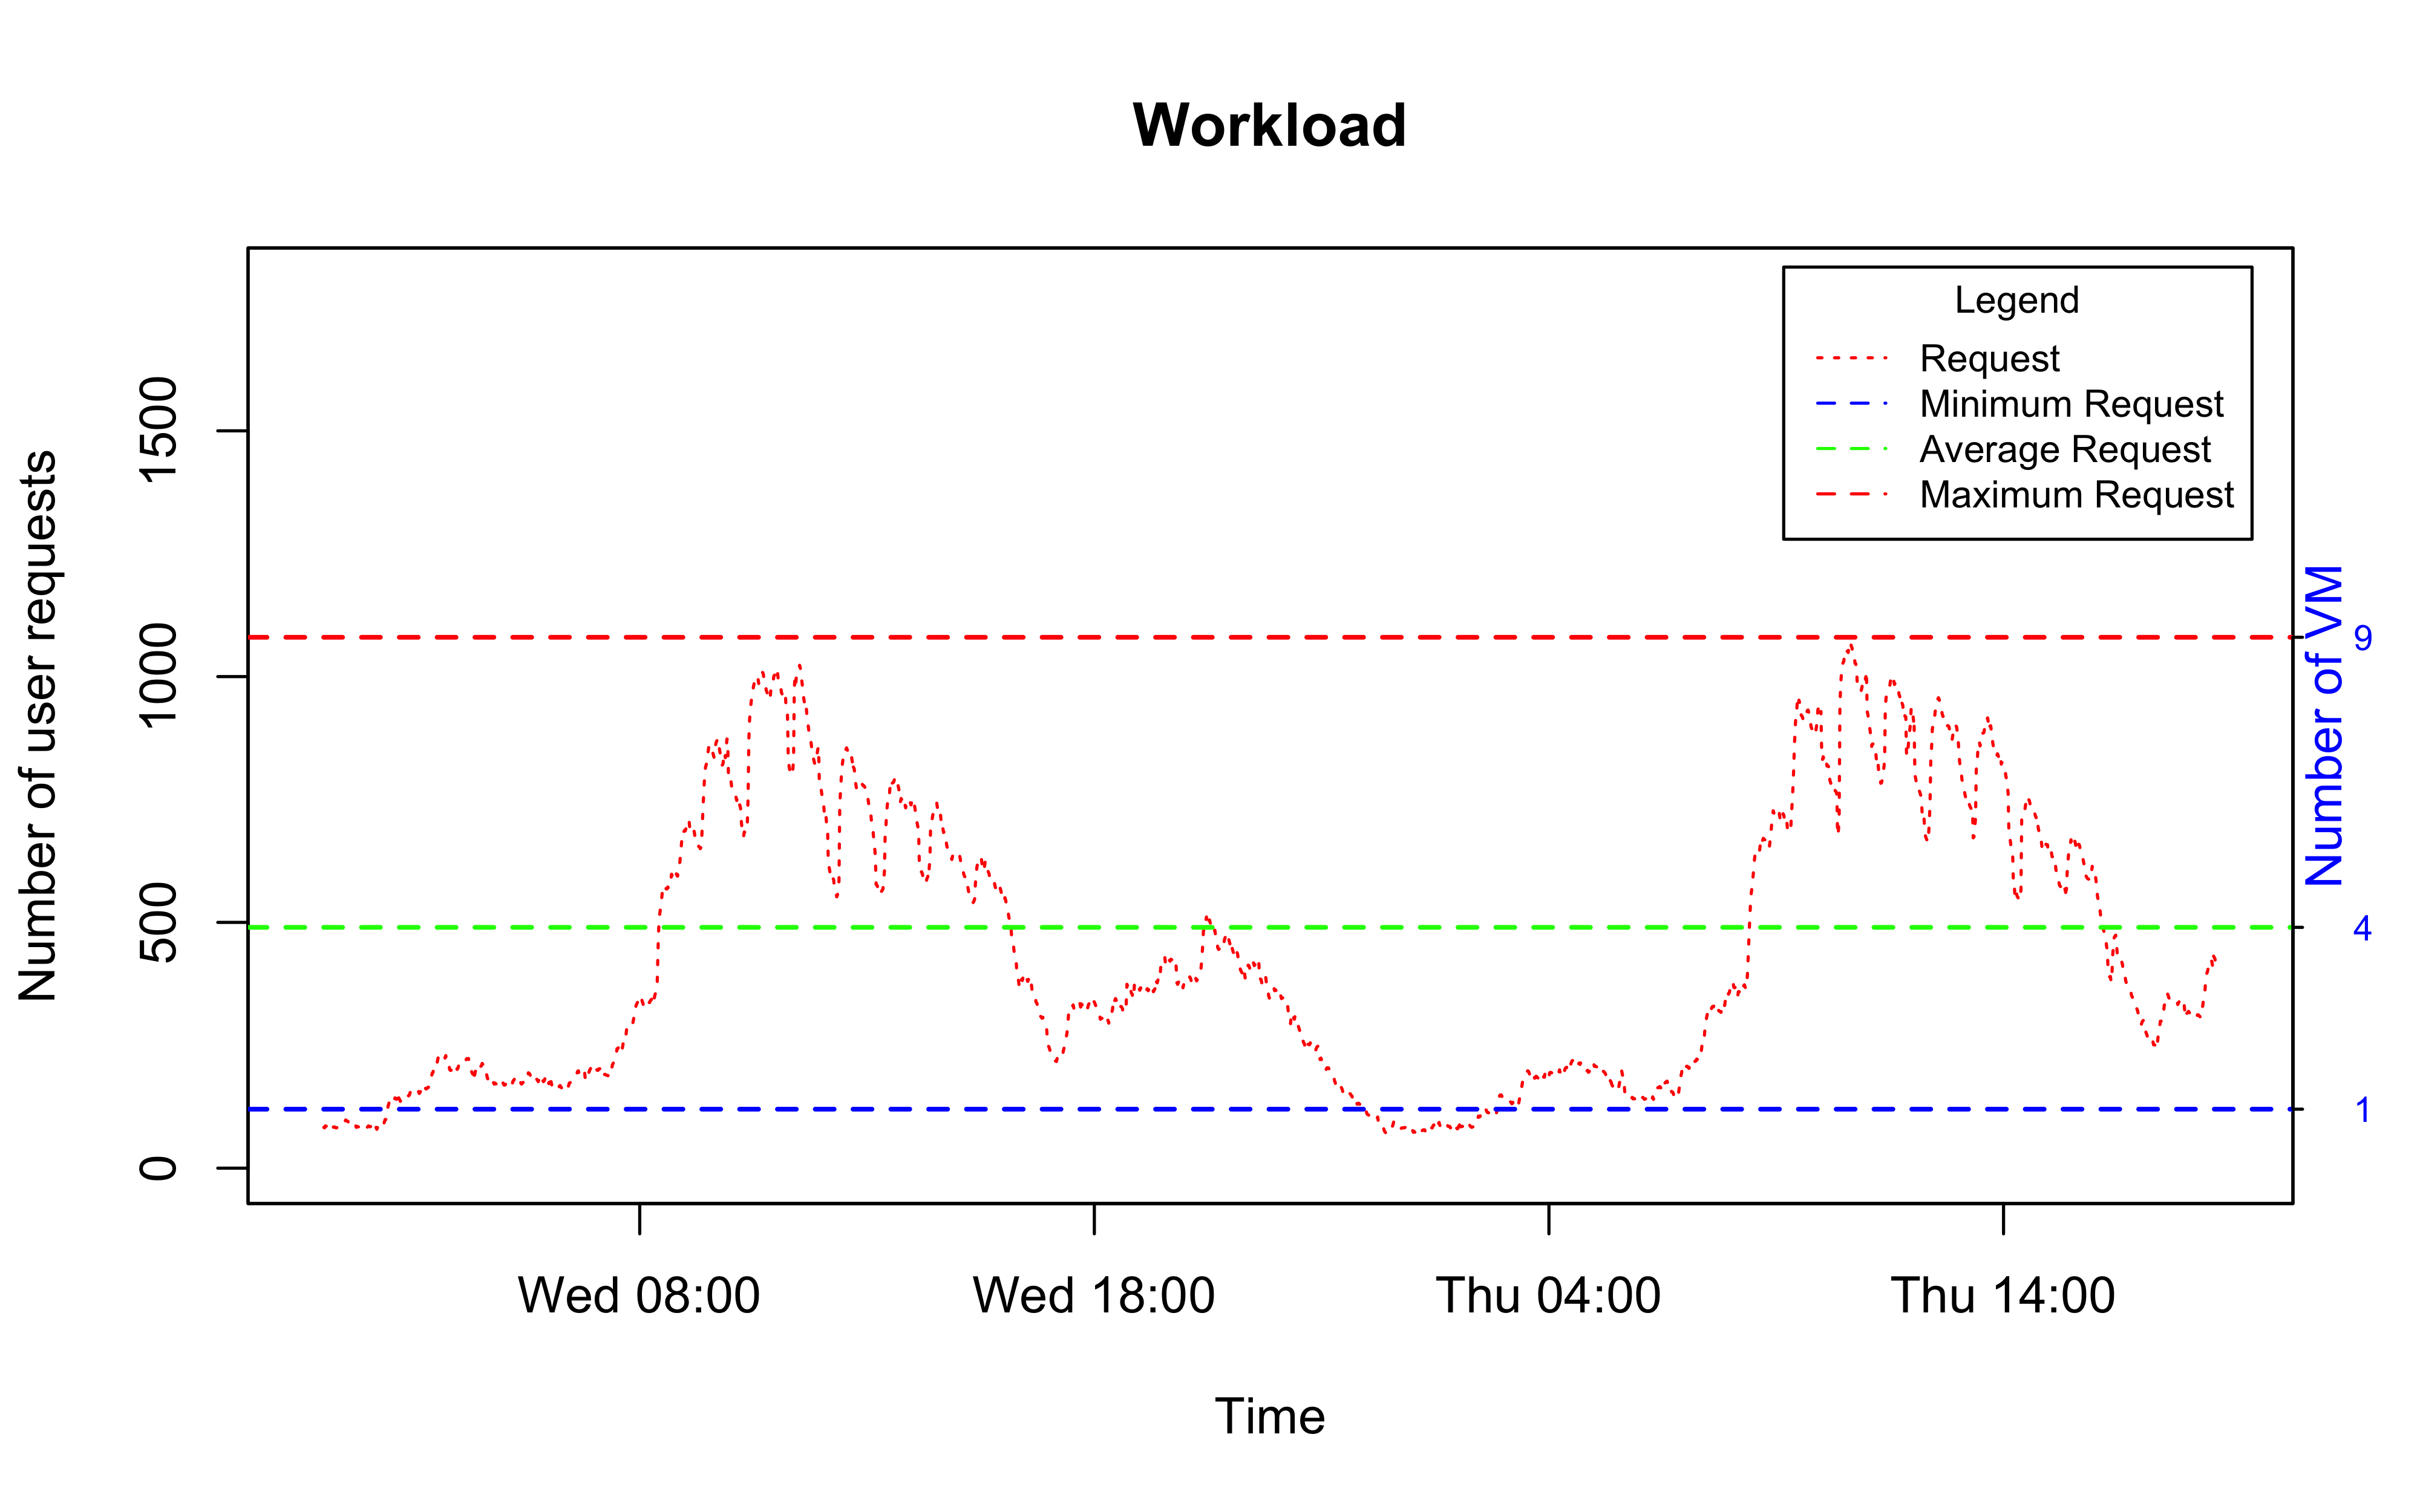
\includegraphics[scale=0.1]{workloadforsim.png}
    \caption{Workload for evaluation}
    \label{figure:workloadforsim}
  \end{center}
\end{figure}
\begin{figure}[h]
  \begin{center}
    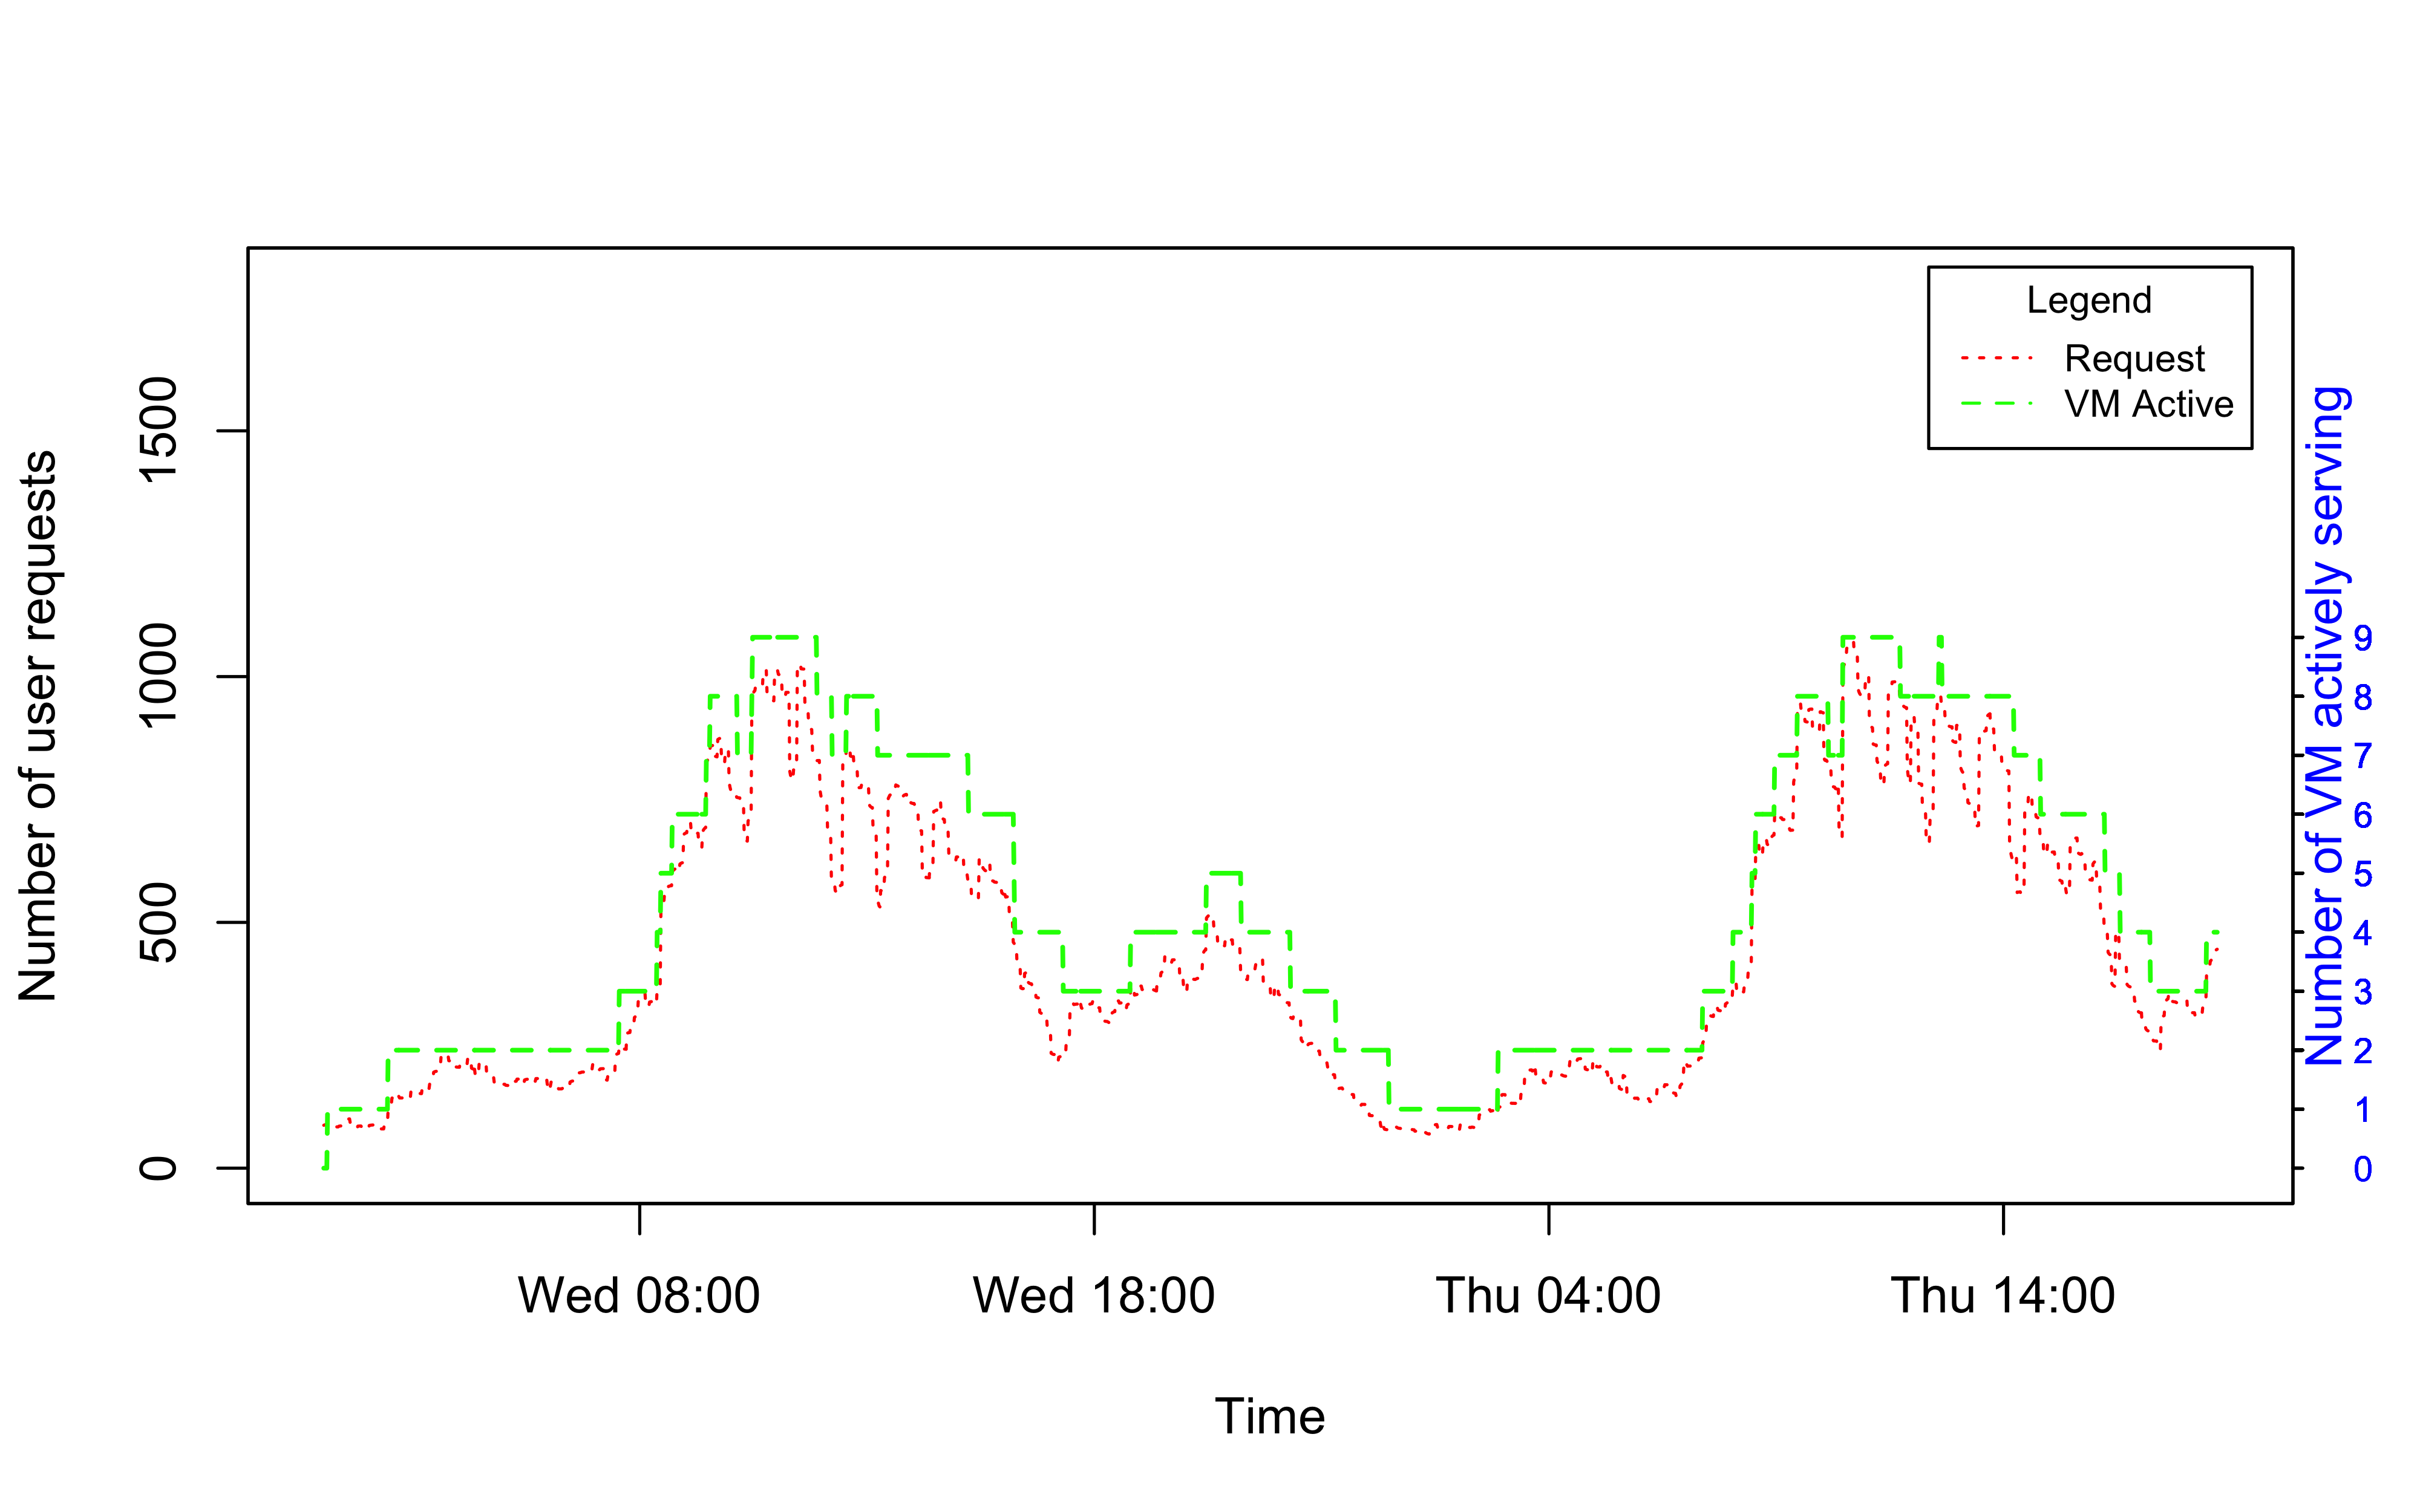
\includegraphics[scale=0.1]{highlevelvmscaling.png}
    \caption{AppElastic applied on input workload}
    \label{figure:appelasticapplication}
  \end{center}
\end{figure}
\subsection{Evaluation of AppElastic Algorithm}
\label{sub:Evaluation of AppElastic Algorithm}
A very important property to define when introducing a new algorithm is its correctness properties. To assert an algorithm is correct it should perform the task as per the specified requirements. To identify a mathematical model as correctness proof is out of scope of this thesis. However, its important to defined the correctness condition for finding the correctness of the algorithm. These correctness conditions will help in identifying any anomaly in the scaling algorithm. For AppElastic algorithm correctness condition can be defined as follows:
\begin{itemize}
  \item On correct execution of the AppElastic algorithm, each VM will be active after some time \(T\) as defined by VM startup time. In other words, the billing period start of the VM should be before its actual start. When a VM is shutdown, it take some time \(T\) as defined by VM shutdown time. Hence, when VM is shutdown at \(T_{i}\) then it will be stopped billing at time \(T_{i}\) + VM shutdown time. These both conditions can be verified by examining the log entries and plotting graphs of the data as provided by ElasticSim.
  \item Each VM has capacity of serving \(N\) number of user as specified in the \(numberOfUserPerInstance\) config option. If there are \(M\) number of users at time \(T\), the number of VM's active at time \(T\) should have the capacity to handle \(M\) users at time \(T\). And this capacity is given by the formula:
  \begin{equation}
    Capaticy_{t} = VM Active_{T} * \textrm{numberOfUsersPerInstance}
  \end{equation}
\end{itemize}

On the correct execution of AppElastic algorithm, above said conditions has to be fulfilled. To show whether AppElastic meets the first condition, Figure~\ref{figure:billingactivescaleup} and Figure~\ref{figure:billingactivescaledown} are presented. In these figures red dotted lines represents the input workload trace, blue line show VM's which are billing and green line shows these VM's which are active for user request. From Figure~\ref{figure:billingactivescaleup} its evident that AppElastic algorithm consider the delay in starting the VM. As its shows, VM's starts billing at 01:02 hours and VM will be active to serve users 5 minutes after at time 01:07 hours. Similarly, from Figure~\ref{figure:billingactivescaledown} its also evident that AppElastic algorithm consider the delay in shutting down of VM's. As shown, VM's stops being active for users at 11:52 hours and VM will ends billing at 12:02 hours.
\\
Figure~\ref{figure:appelasticapplication} shows how VM's are scaled up/down based on the variation in the workload. Red dotted lines represents the input workload trace and the green line show the capacity of active VM's serving the workload. Axis on the right hand side denotes the number of VM's being actively serving these request. From the Figures~\ref{fig:appelasticperformance}, AppElastic algorithm always create VM's such that its capacity green line is alway above the red line user requests. With these two properties, we proved that AppElastic algorithm perform scaling operation as per its requirements.

\begin{figure}
     \centering
     \begin{subfigure}[b]{1.0\textwidth}
         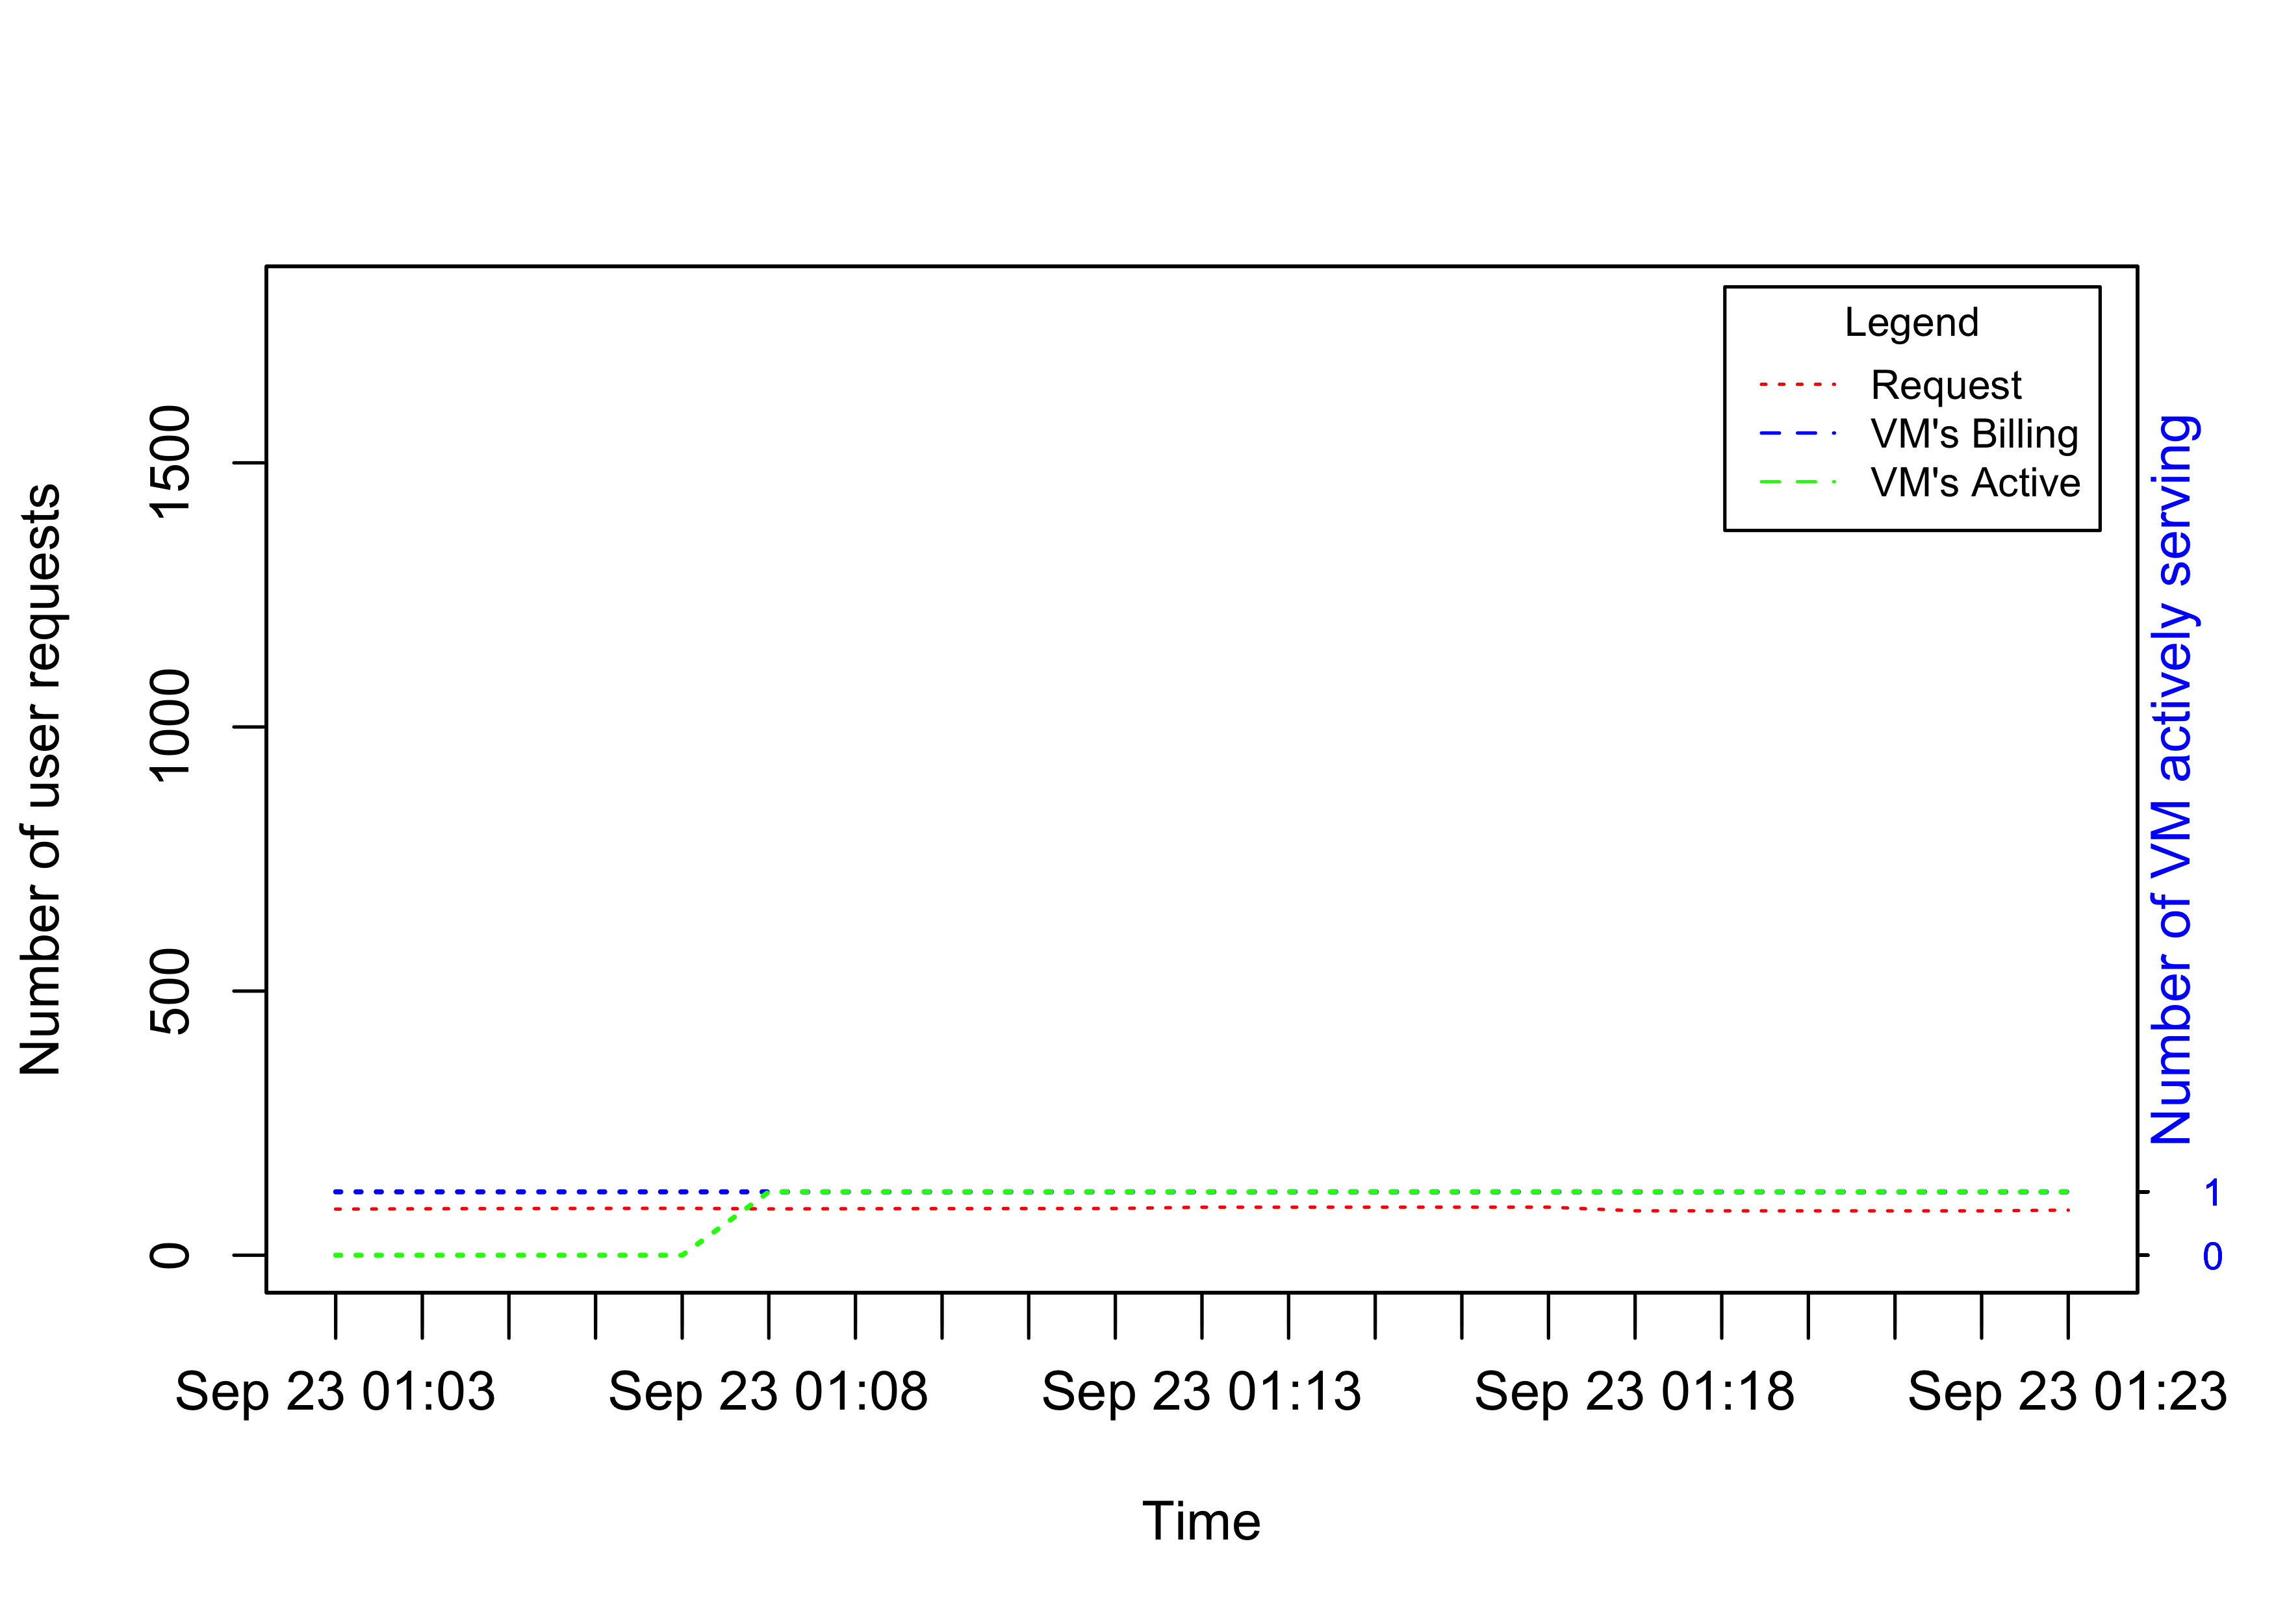
\includegraphics[width=\textwidth]{autoscalingdiagscaleup.png}
         \caption{Scale up: Showing time delay for VM to be active}
         \label{figure:billingactivescaleup}
     \end{subfigure}
     \begin{subfigure}[b]{0.9\textwidth}
         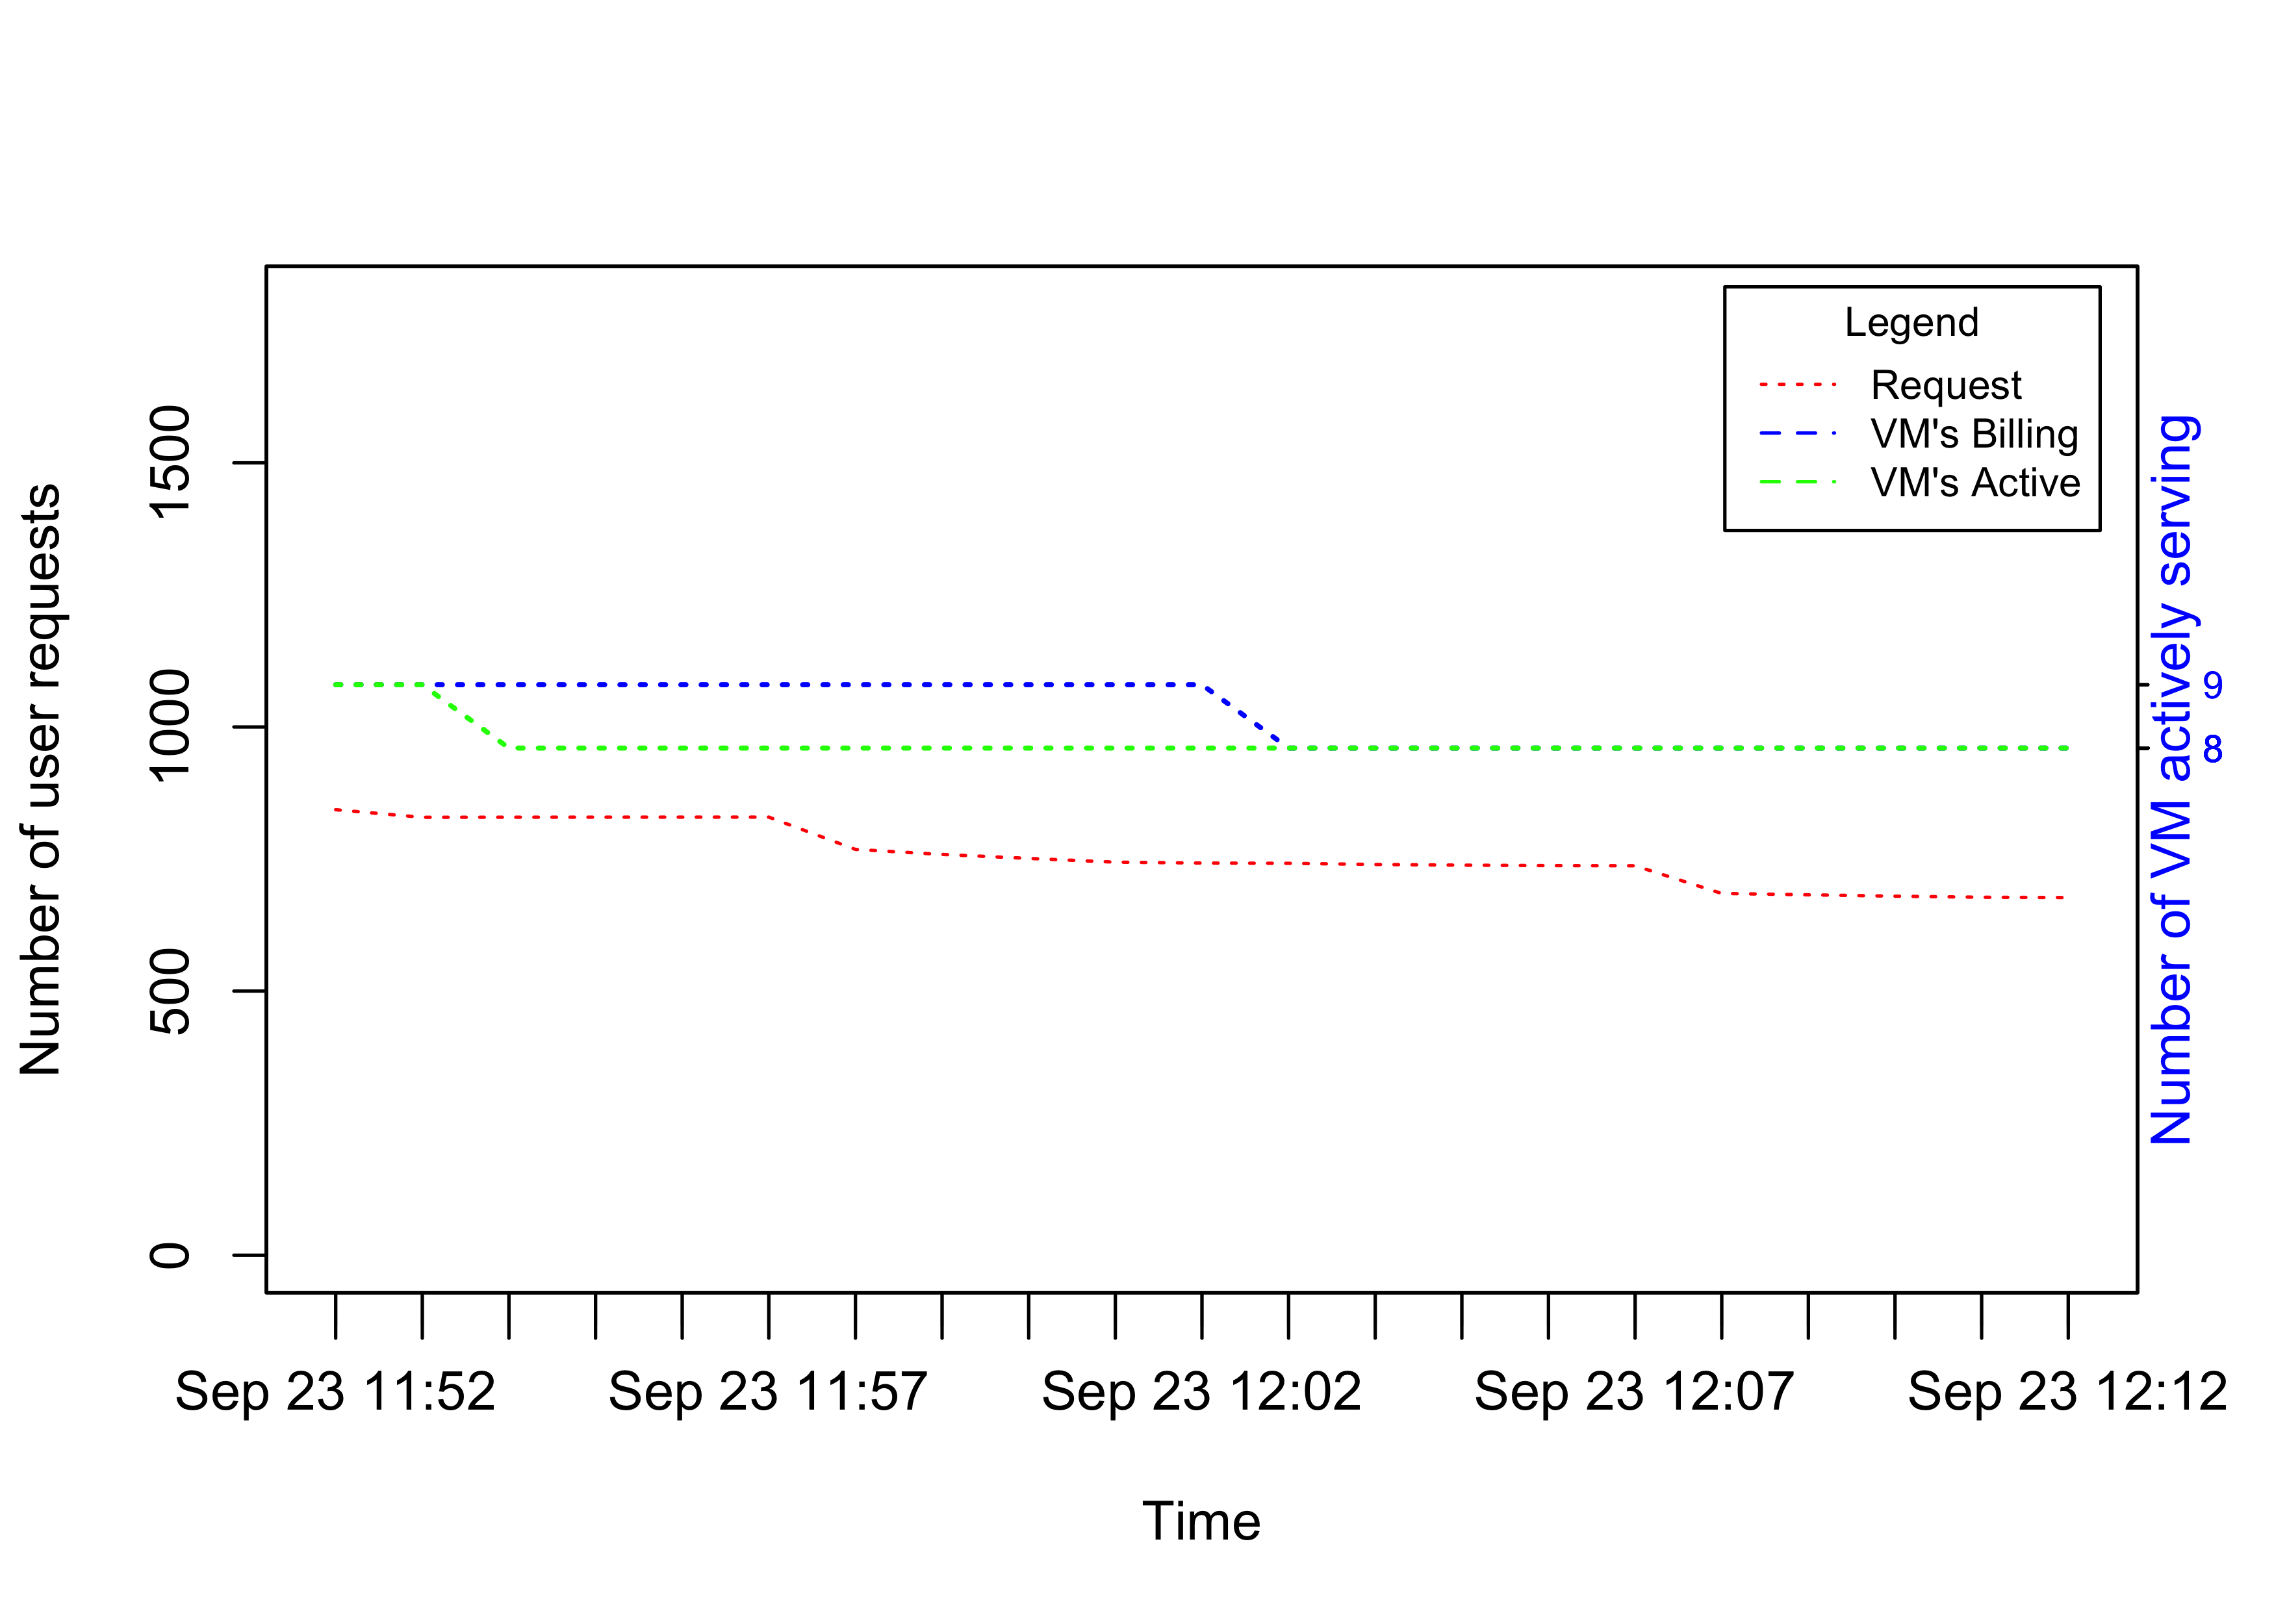
\includegraphics[width=\textwidth]{autoscalingdiagscaledown.png}
         \caption{Scale down: Showing time delay for VM to end billing}
         \label{figure:billingactivescaledown}
     \end{subfigure}
     \caption{Scale Up and Down}
     \label{fig:billingactive}
\end{figure}

\begin{figure}
     \centering
     \begin{subfigure}[b]{0.4\textwidth}
         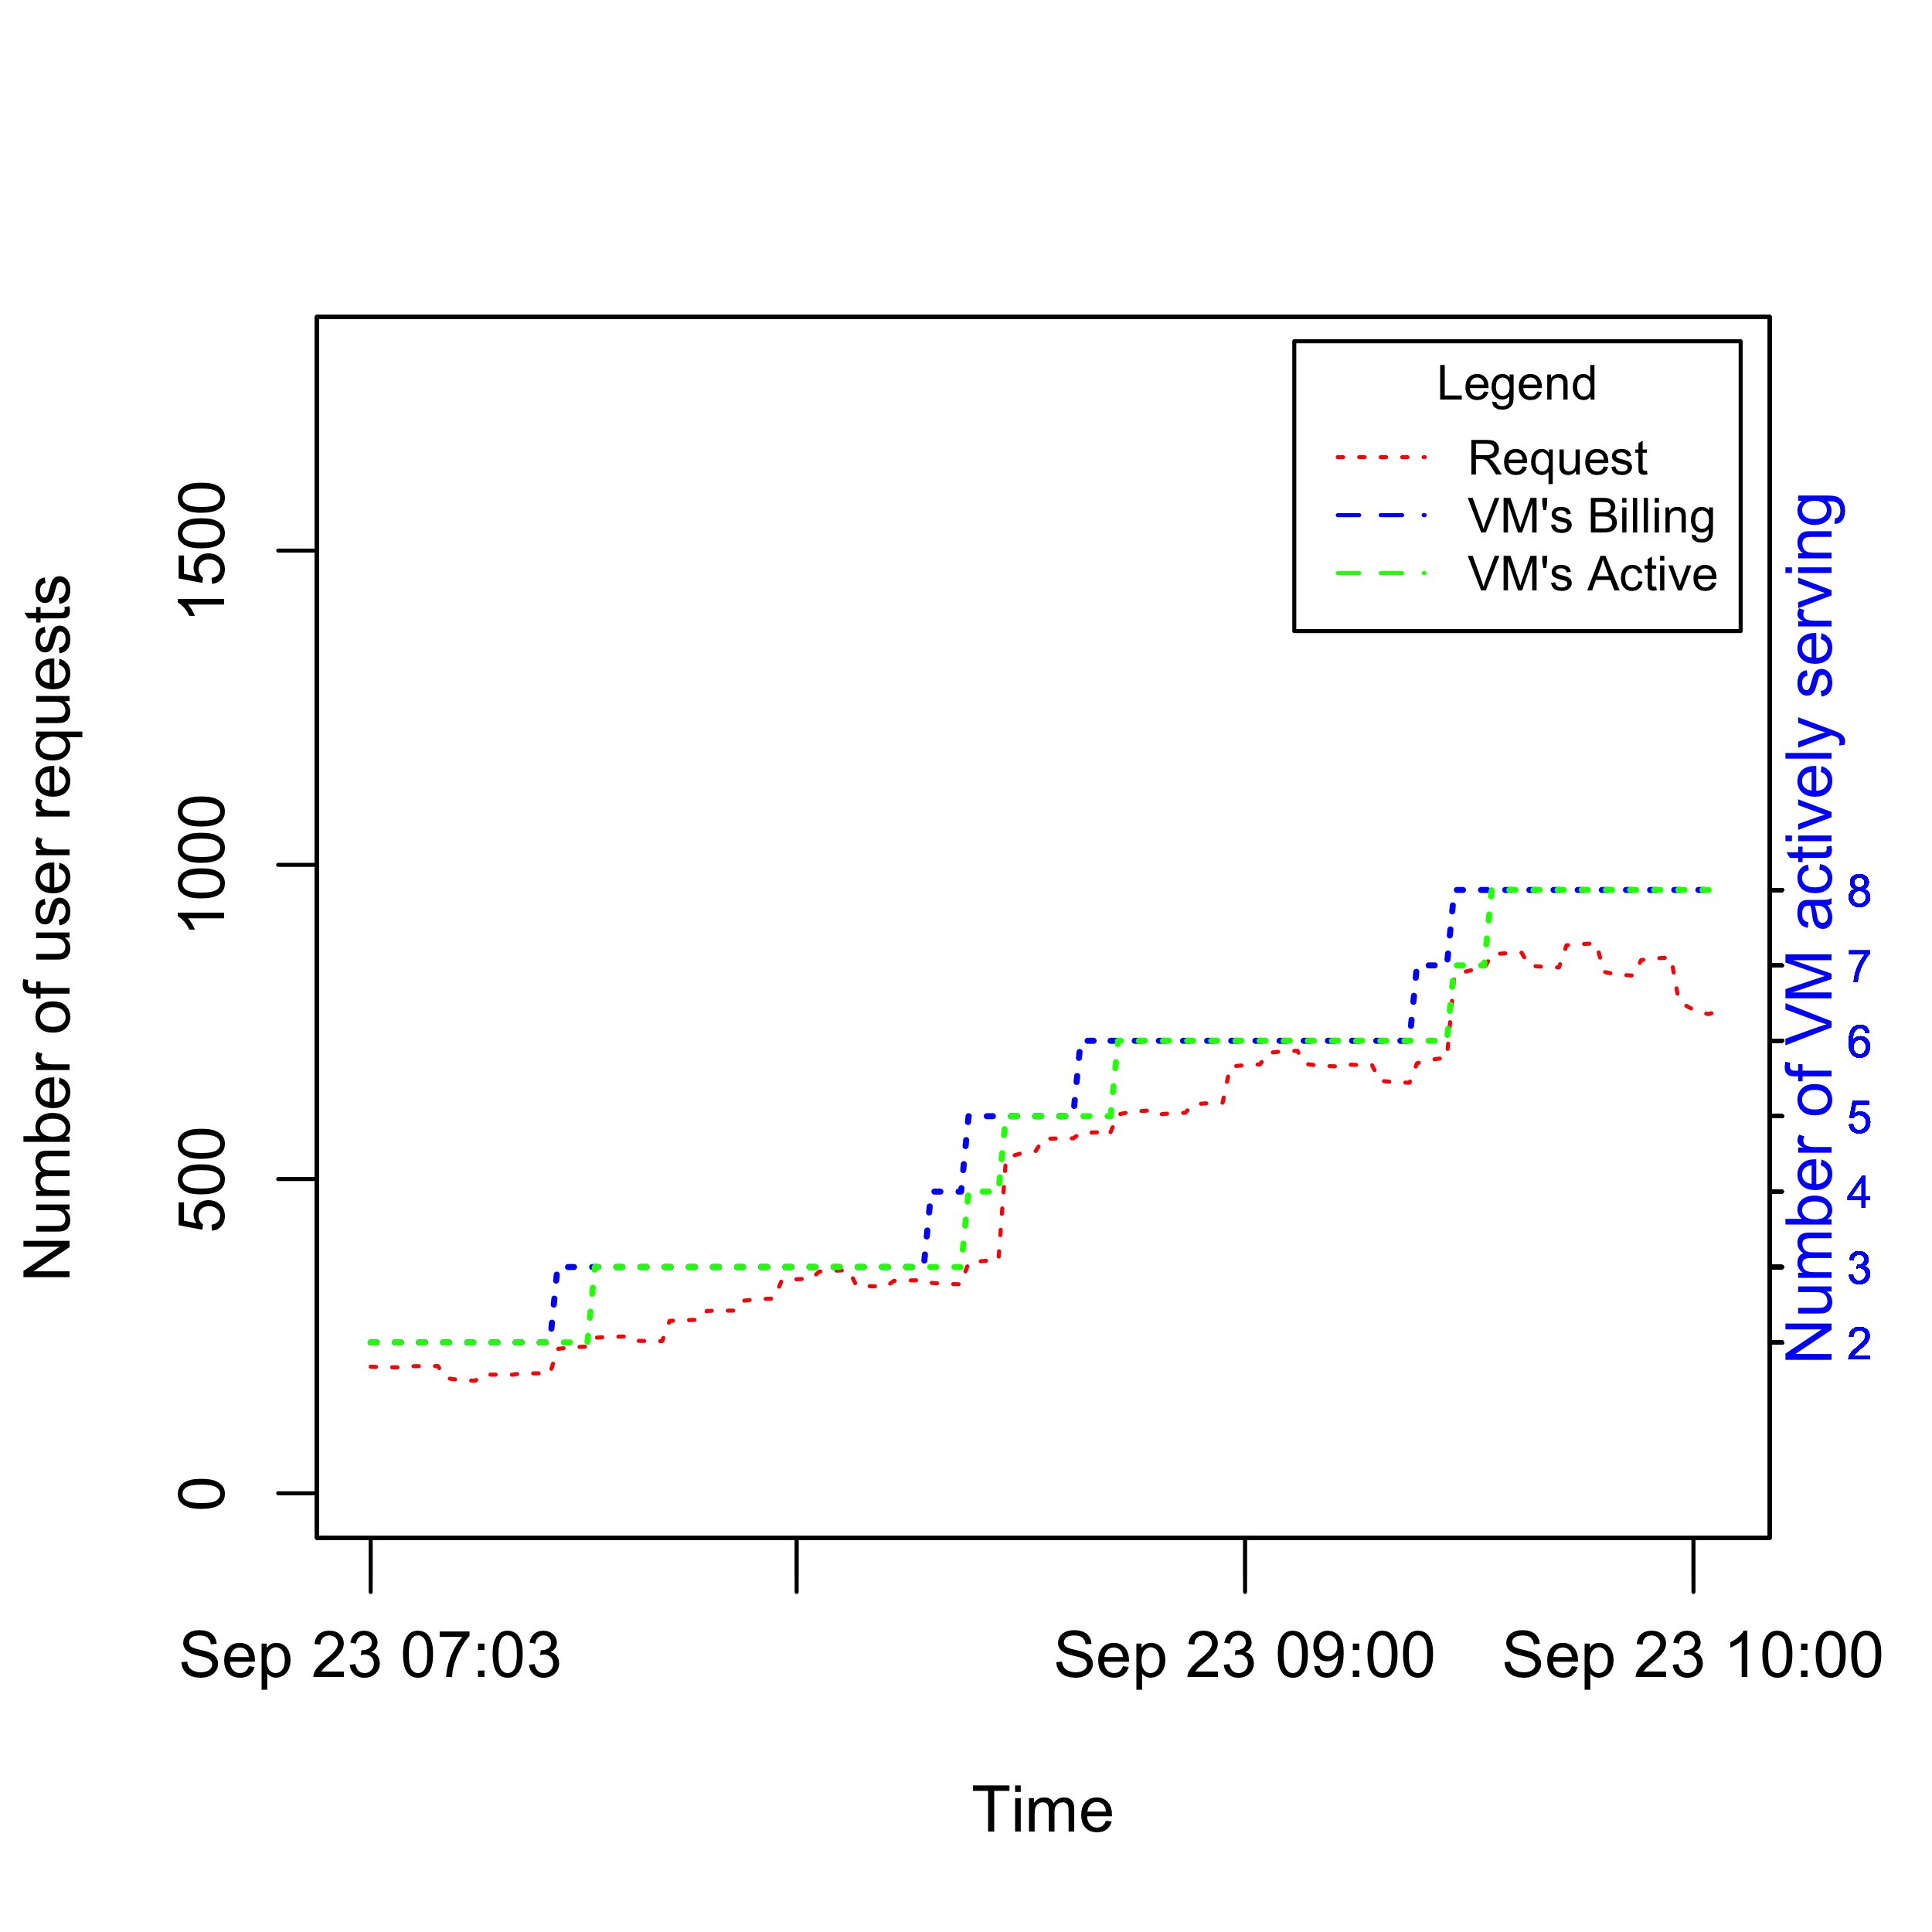
\includegraphics[width=\textwidth]{autoscalingdiag1.png}
         \caption{Increase in user request}
         \label{figure:autoscalingdiag1}
     \end{subfigure}
      \hfill
     \begin{subfigure}[b]{0.4\textwidth}
         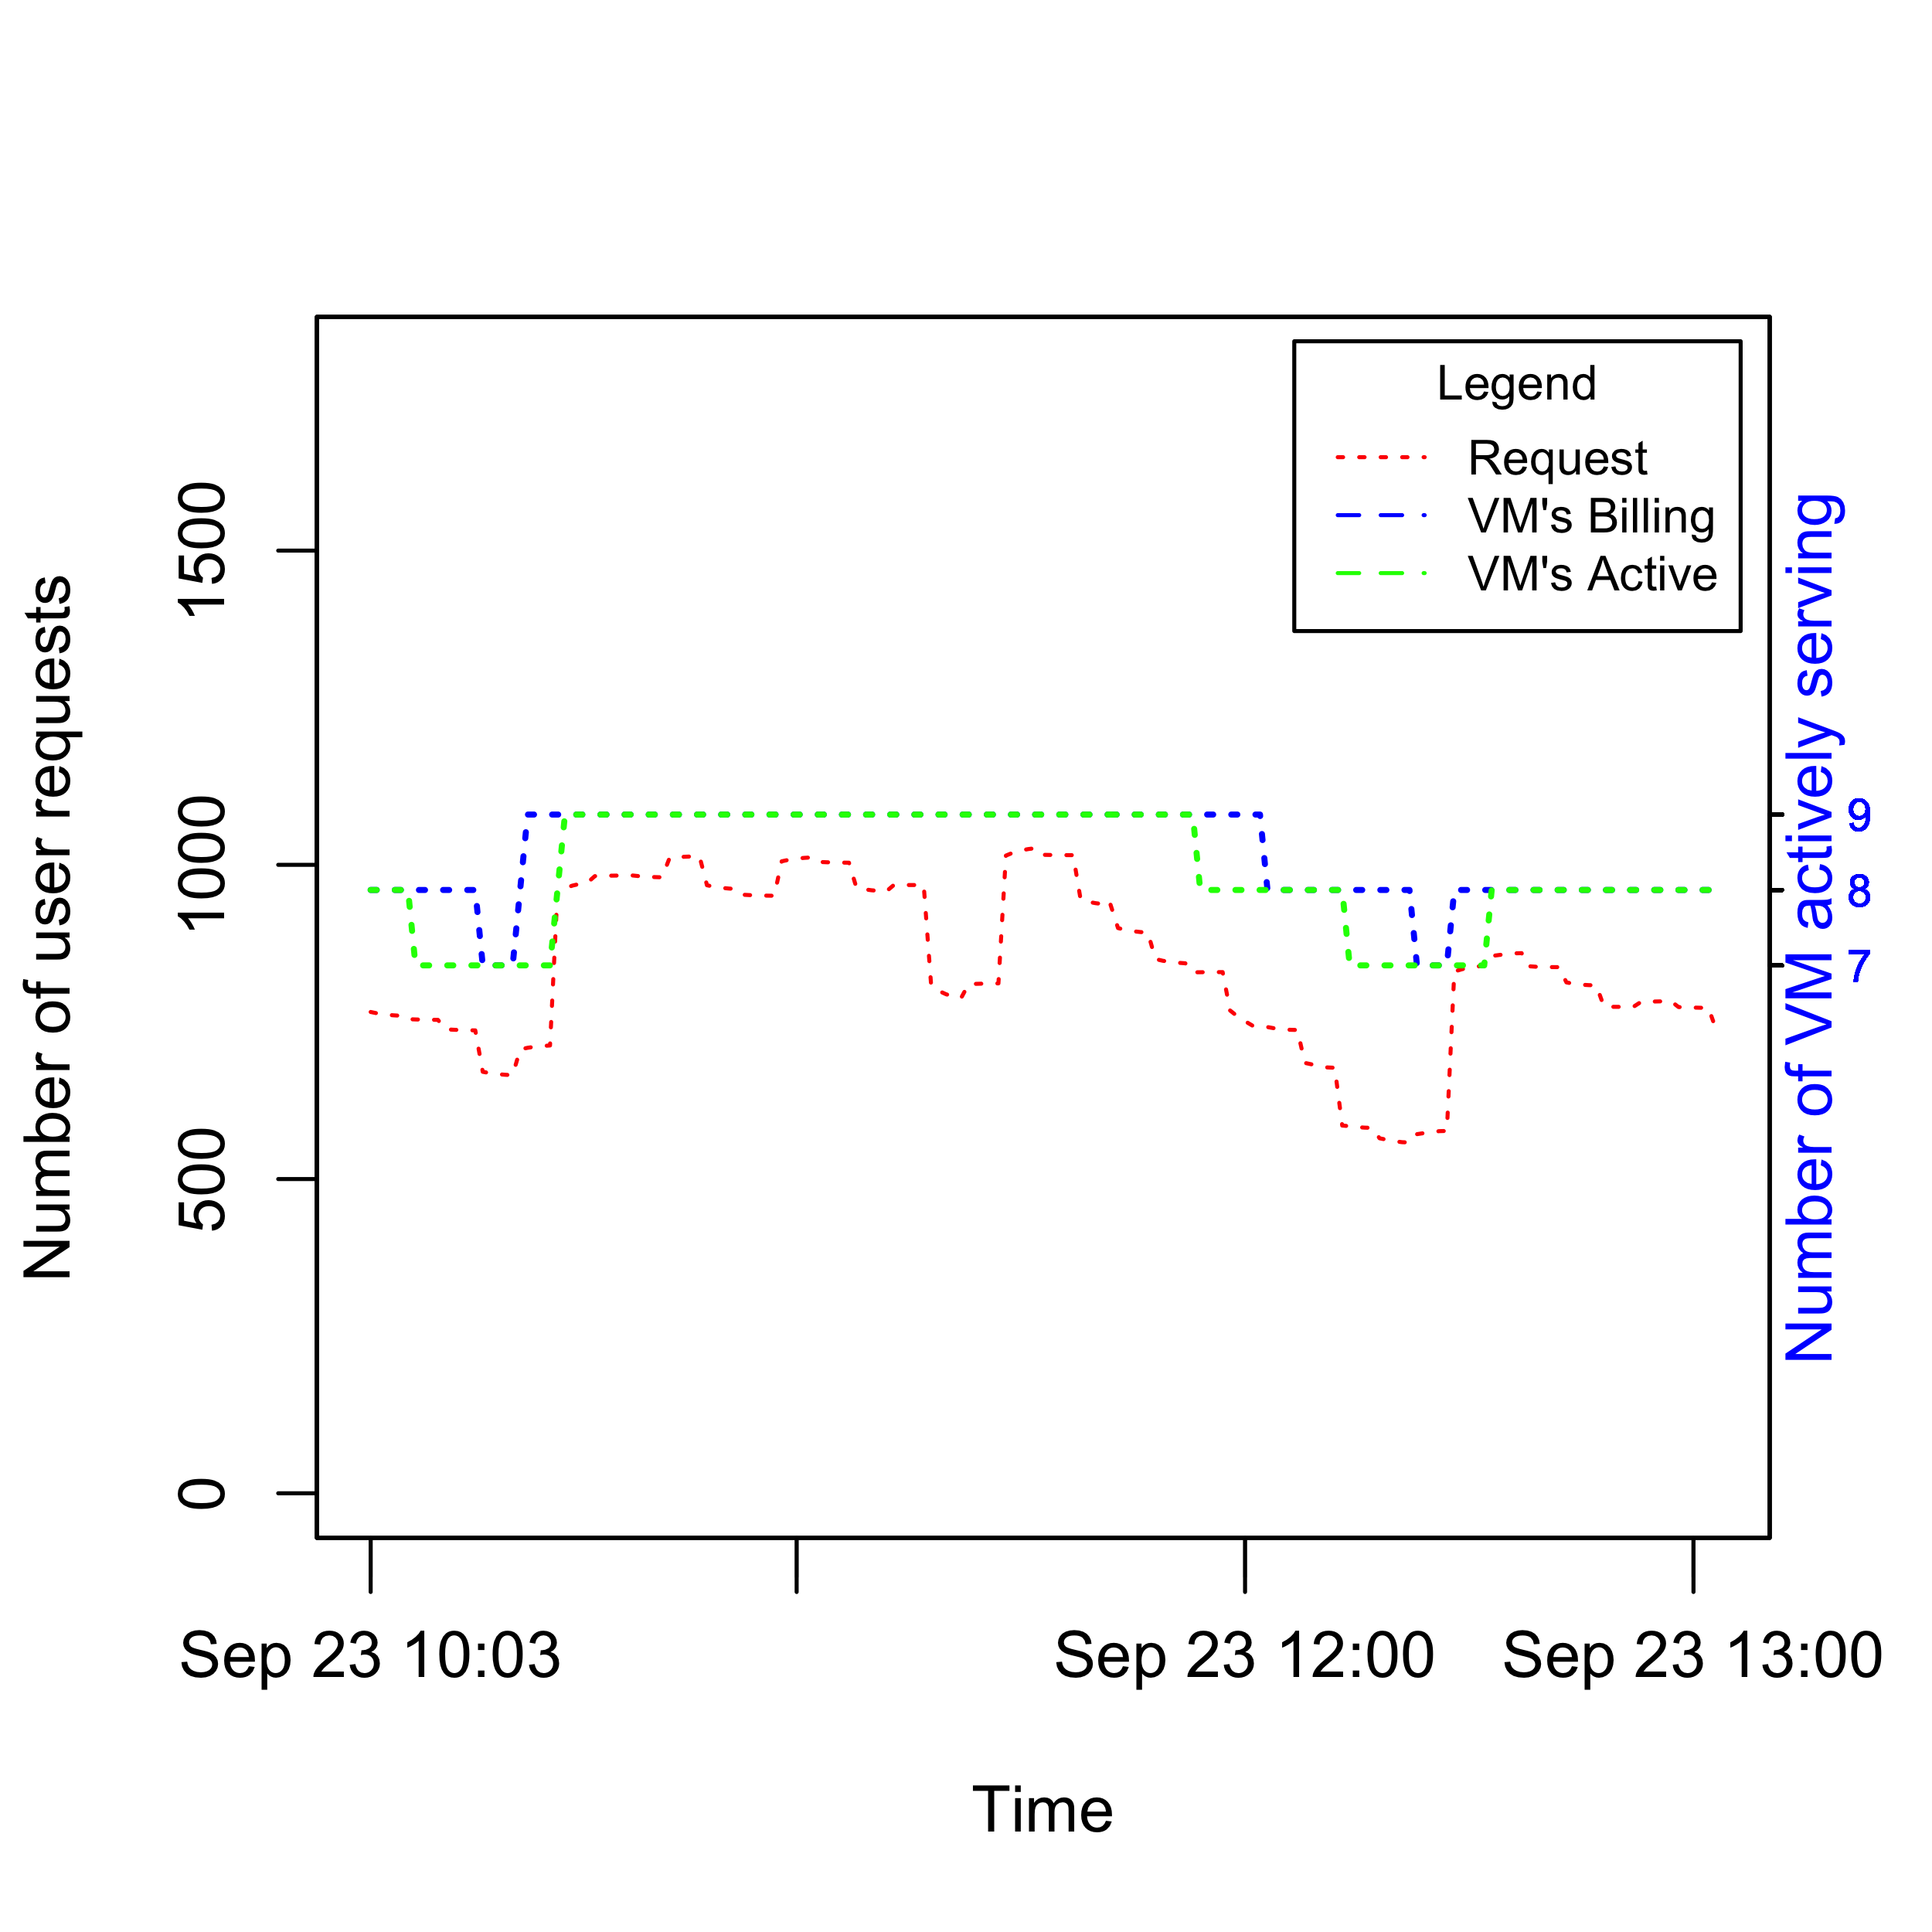
\includegraphics[width=\textwidth]{autoscalingdiag2.png}
         \caption{Rapid change in user request}
         \label{figure:autoscalingdiag2}
     \end{subfigure}
     \vskip\baselineskip
     \begin{subfigure}[b]{0.4\textwidth}
         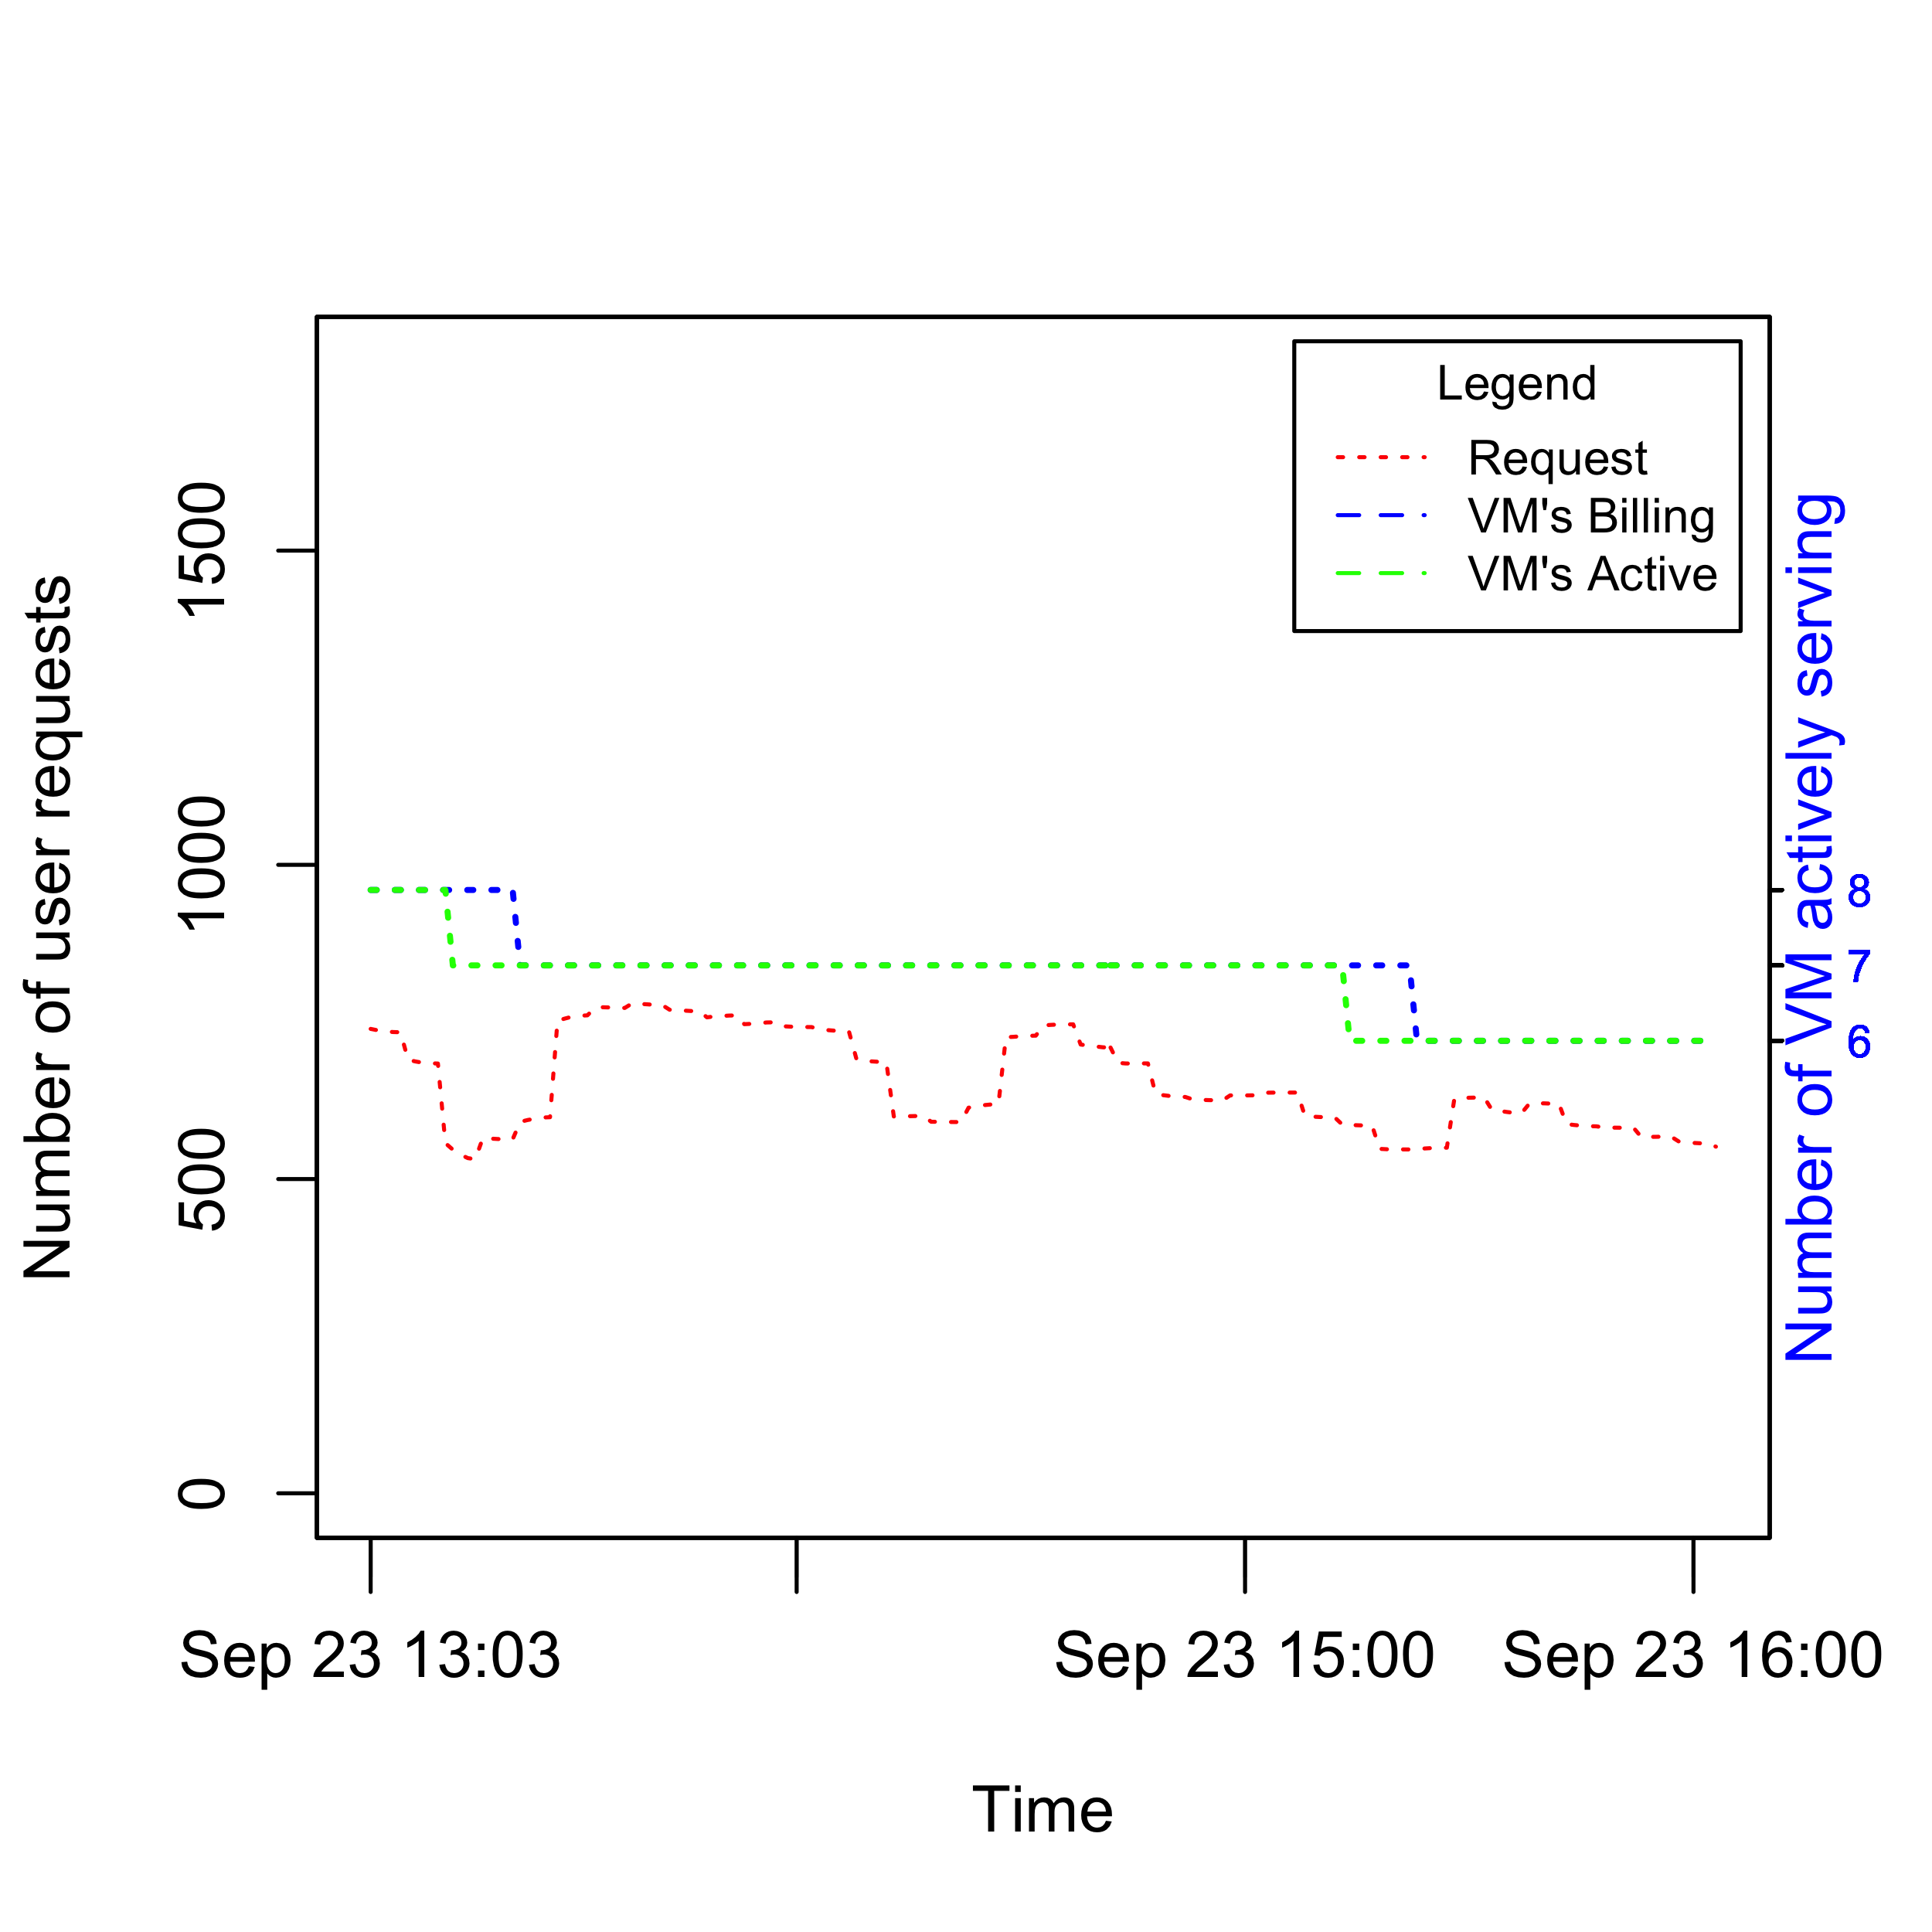
\includegraphics[width=\textwidth]{autoscalingdiag3.png}
         \caption{Decreasing in user request}
         \label{figure:autoscalingdiag3}
     \end{subfigure}
      \hfill
     \begin{subfigure}[b]{0.4\textwidth}
         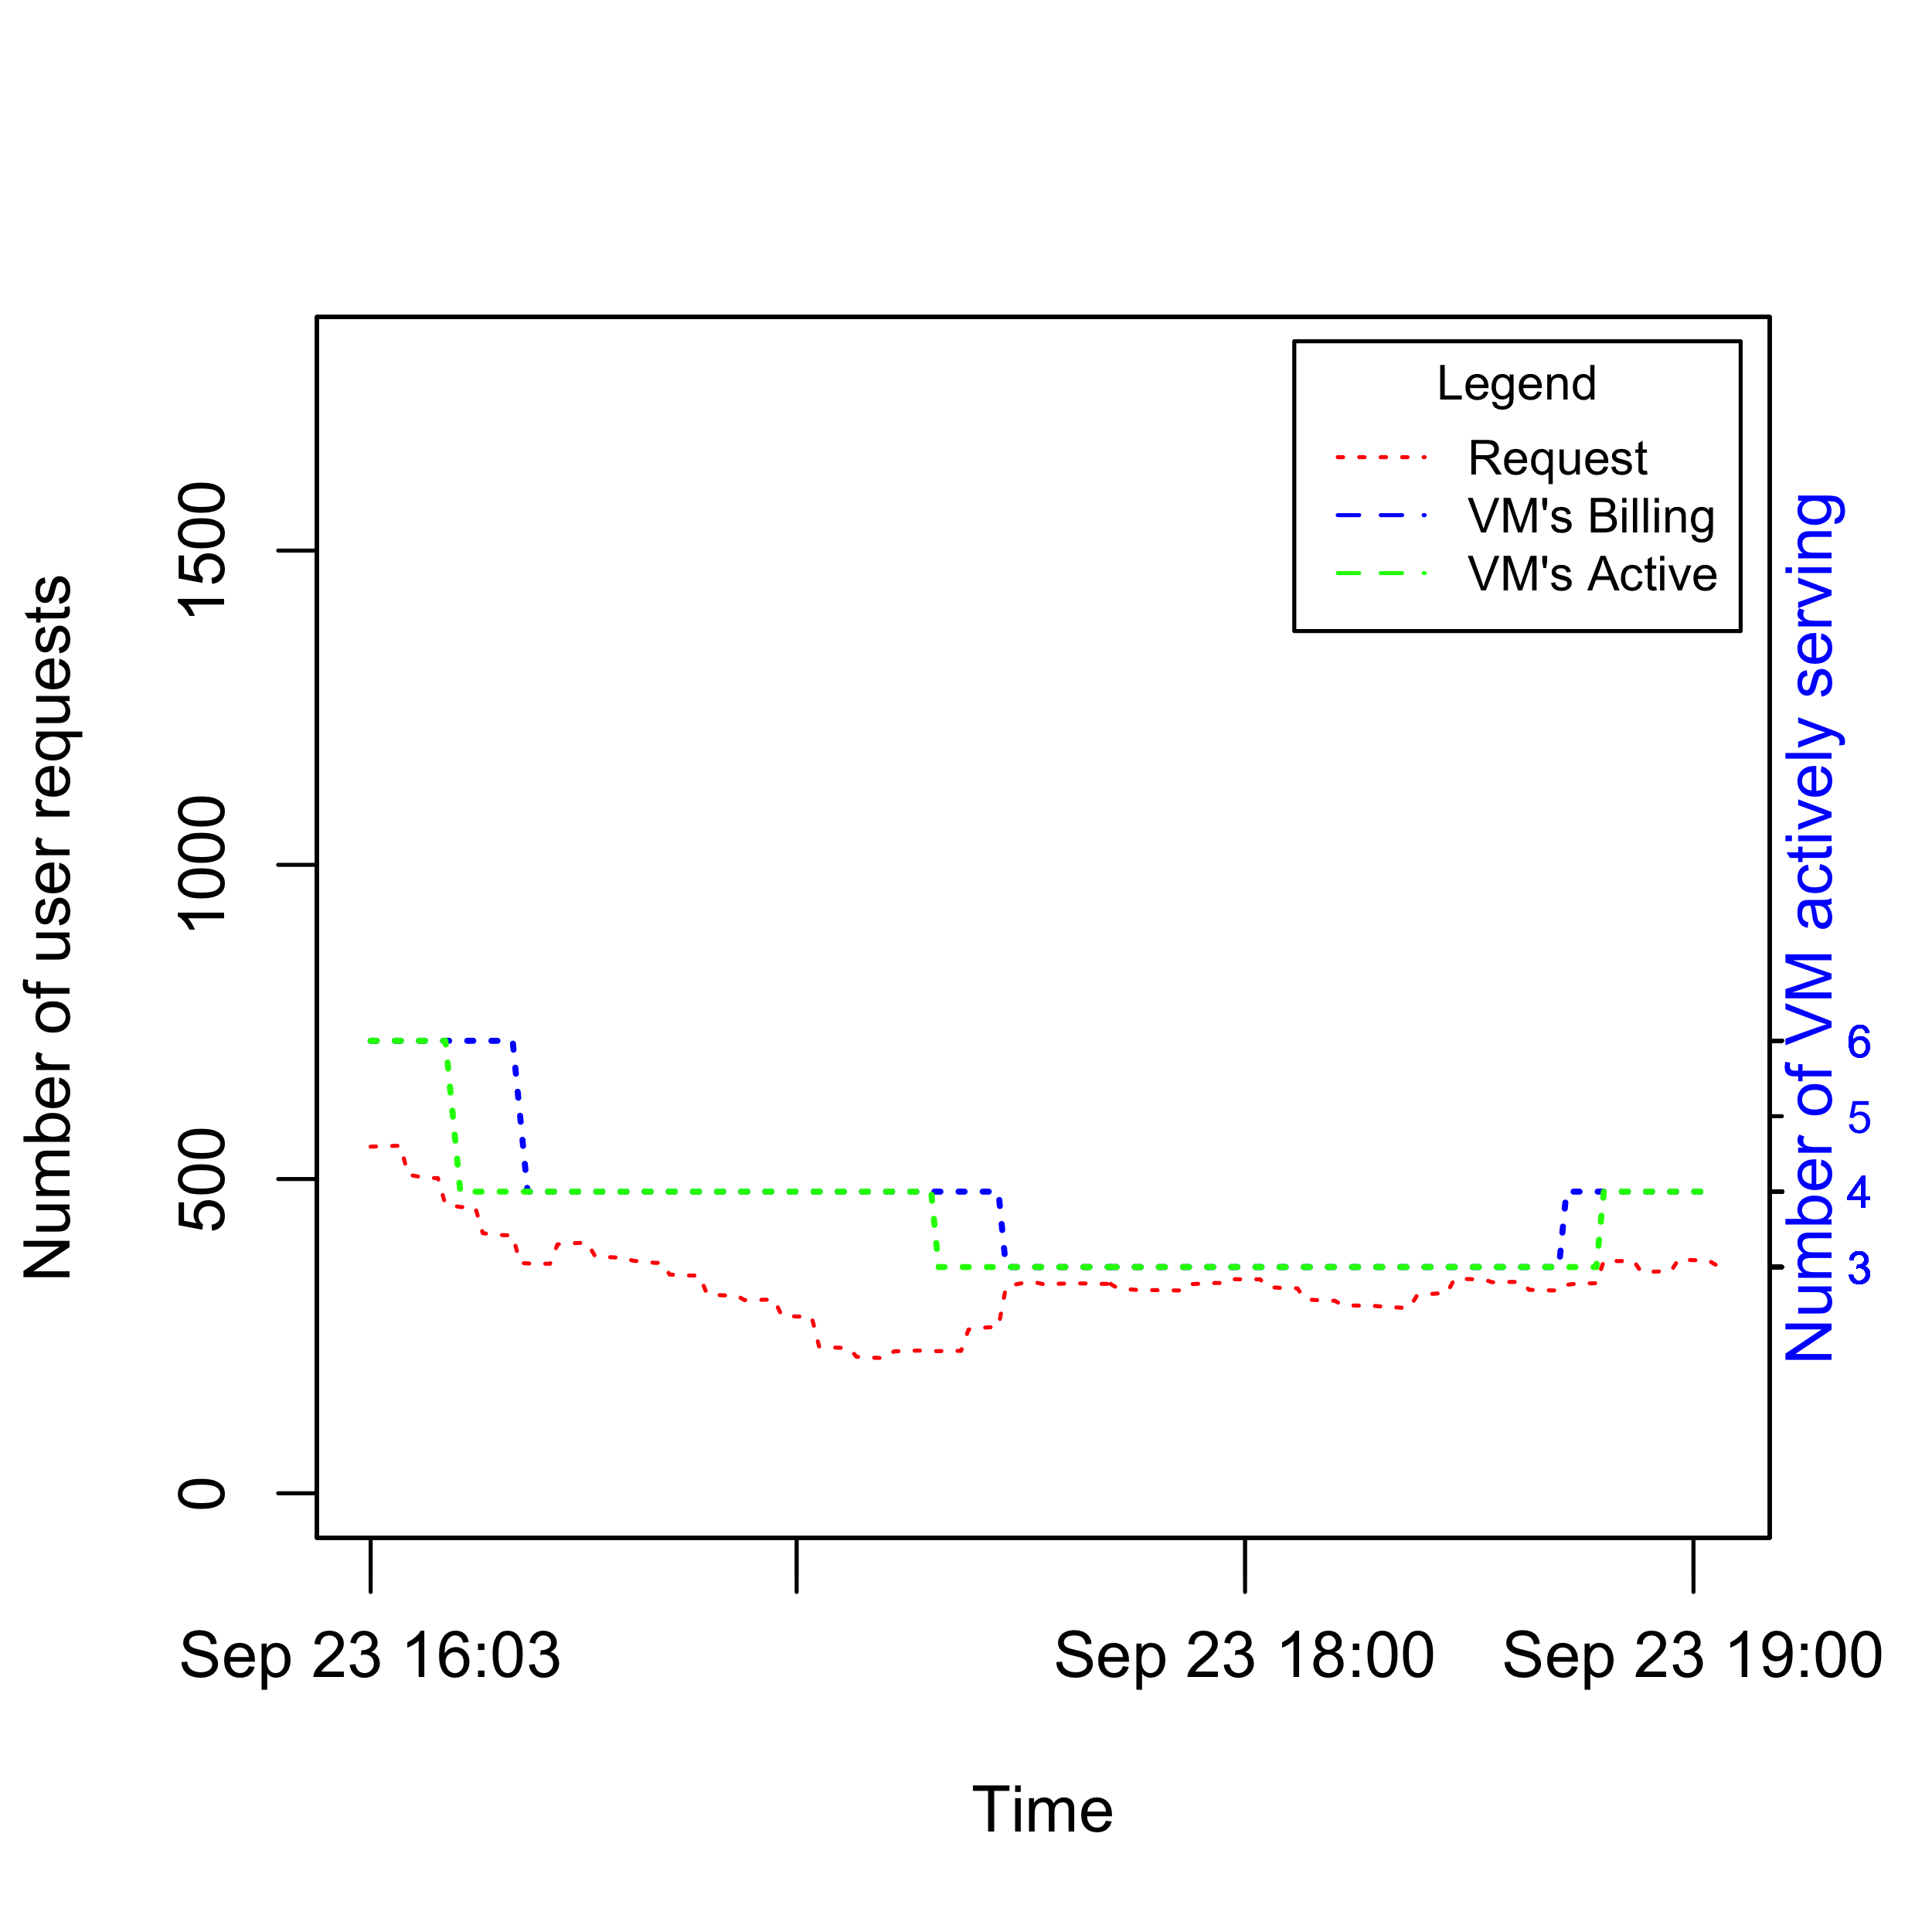
\includegraphics[width=\textwidth]{autoscalingdiag4.png}
         \caption{Decreasing in user request}
         \label{figure:autoscalingdiag4}
     \end{subfigure}
     \caption{AppElastic Performace on Workload}
     \label{fig:appelasticperformance}
 \end{figure}

\subsection{Forecast Accuracy}
\label{sub:Forecast Accuracy}
As discussed in the previous chapter, automated ARIMA model is used to forecast two type of data. These forecast data aids AppElastic for scale up lookahead and scale down lookahead features. Figure~\ref{fig:forecast} show the forecast plot of actual number of user request along with forecasted values. Based on the forecast horizon specified in ElasticSim configuration, forecasts are produced for scale up in Figure~\ref{figure:forecastscaleup} and for scale down as shown in Figure~\ref{figure:forecastscaledown}. As introduced in section~\ref{sec:implementationprediction} percentage error is used to measured the accuracy. MAPE Percentage errors have the advantage of being scale-independent, and frequently used to compare forecast performance between different data sets. Box plot of forecast errors are as shown in Figure~\ref{fig:forecasterror}. Using automated ARIMA modeling building with R \(auto.arima()\) function has produced forecast with mean error of 1.5\% in both scale up and scale down forecasts. In section~\ref{sub:SLA violation}, how this error in forecast model affects the SLA is presented.
\begin{figure}
     \centering
     \begin{subfigure}[b]{0.9\textwidth}
         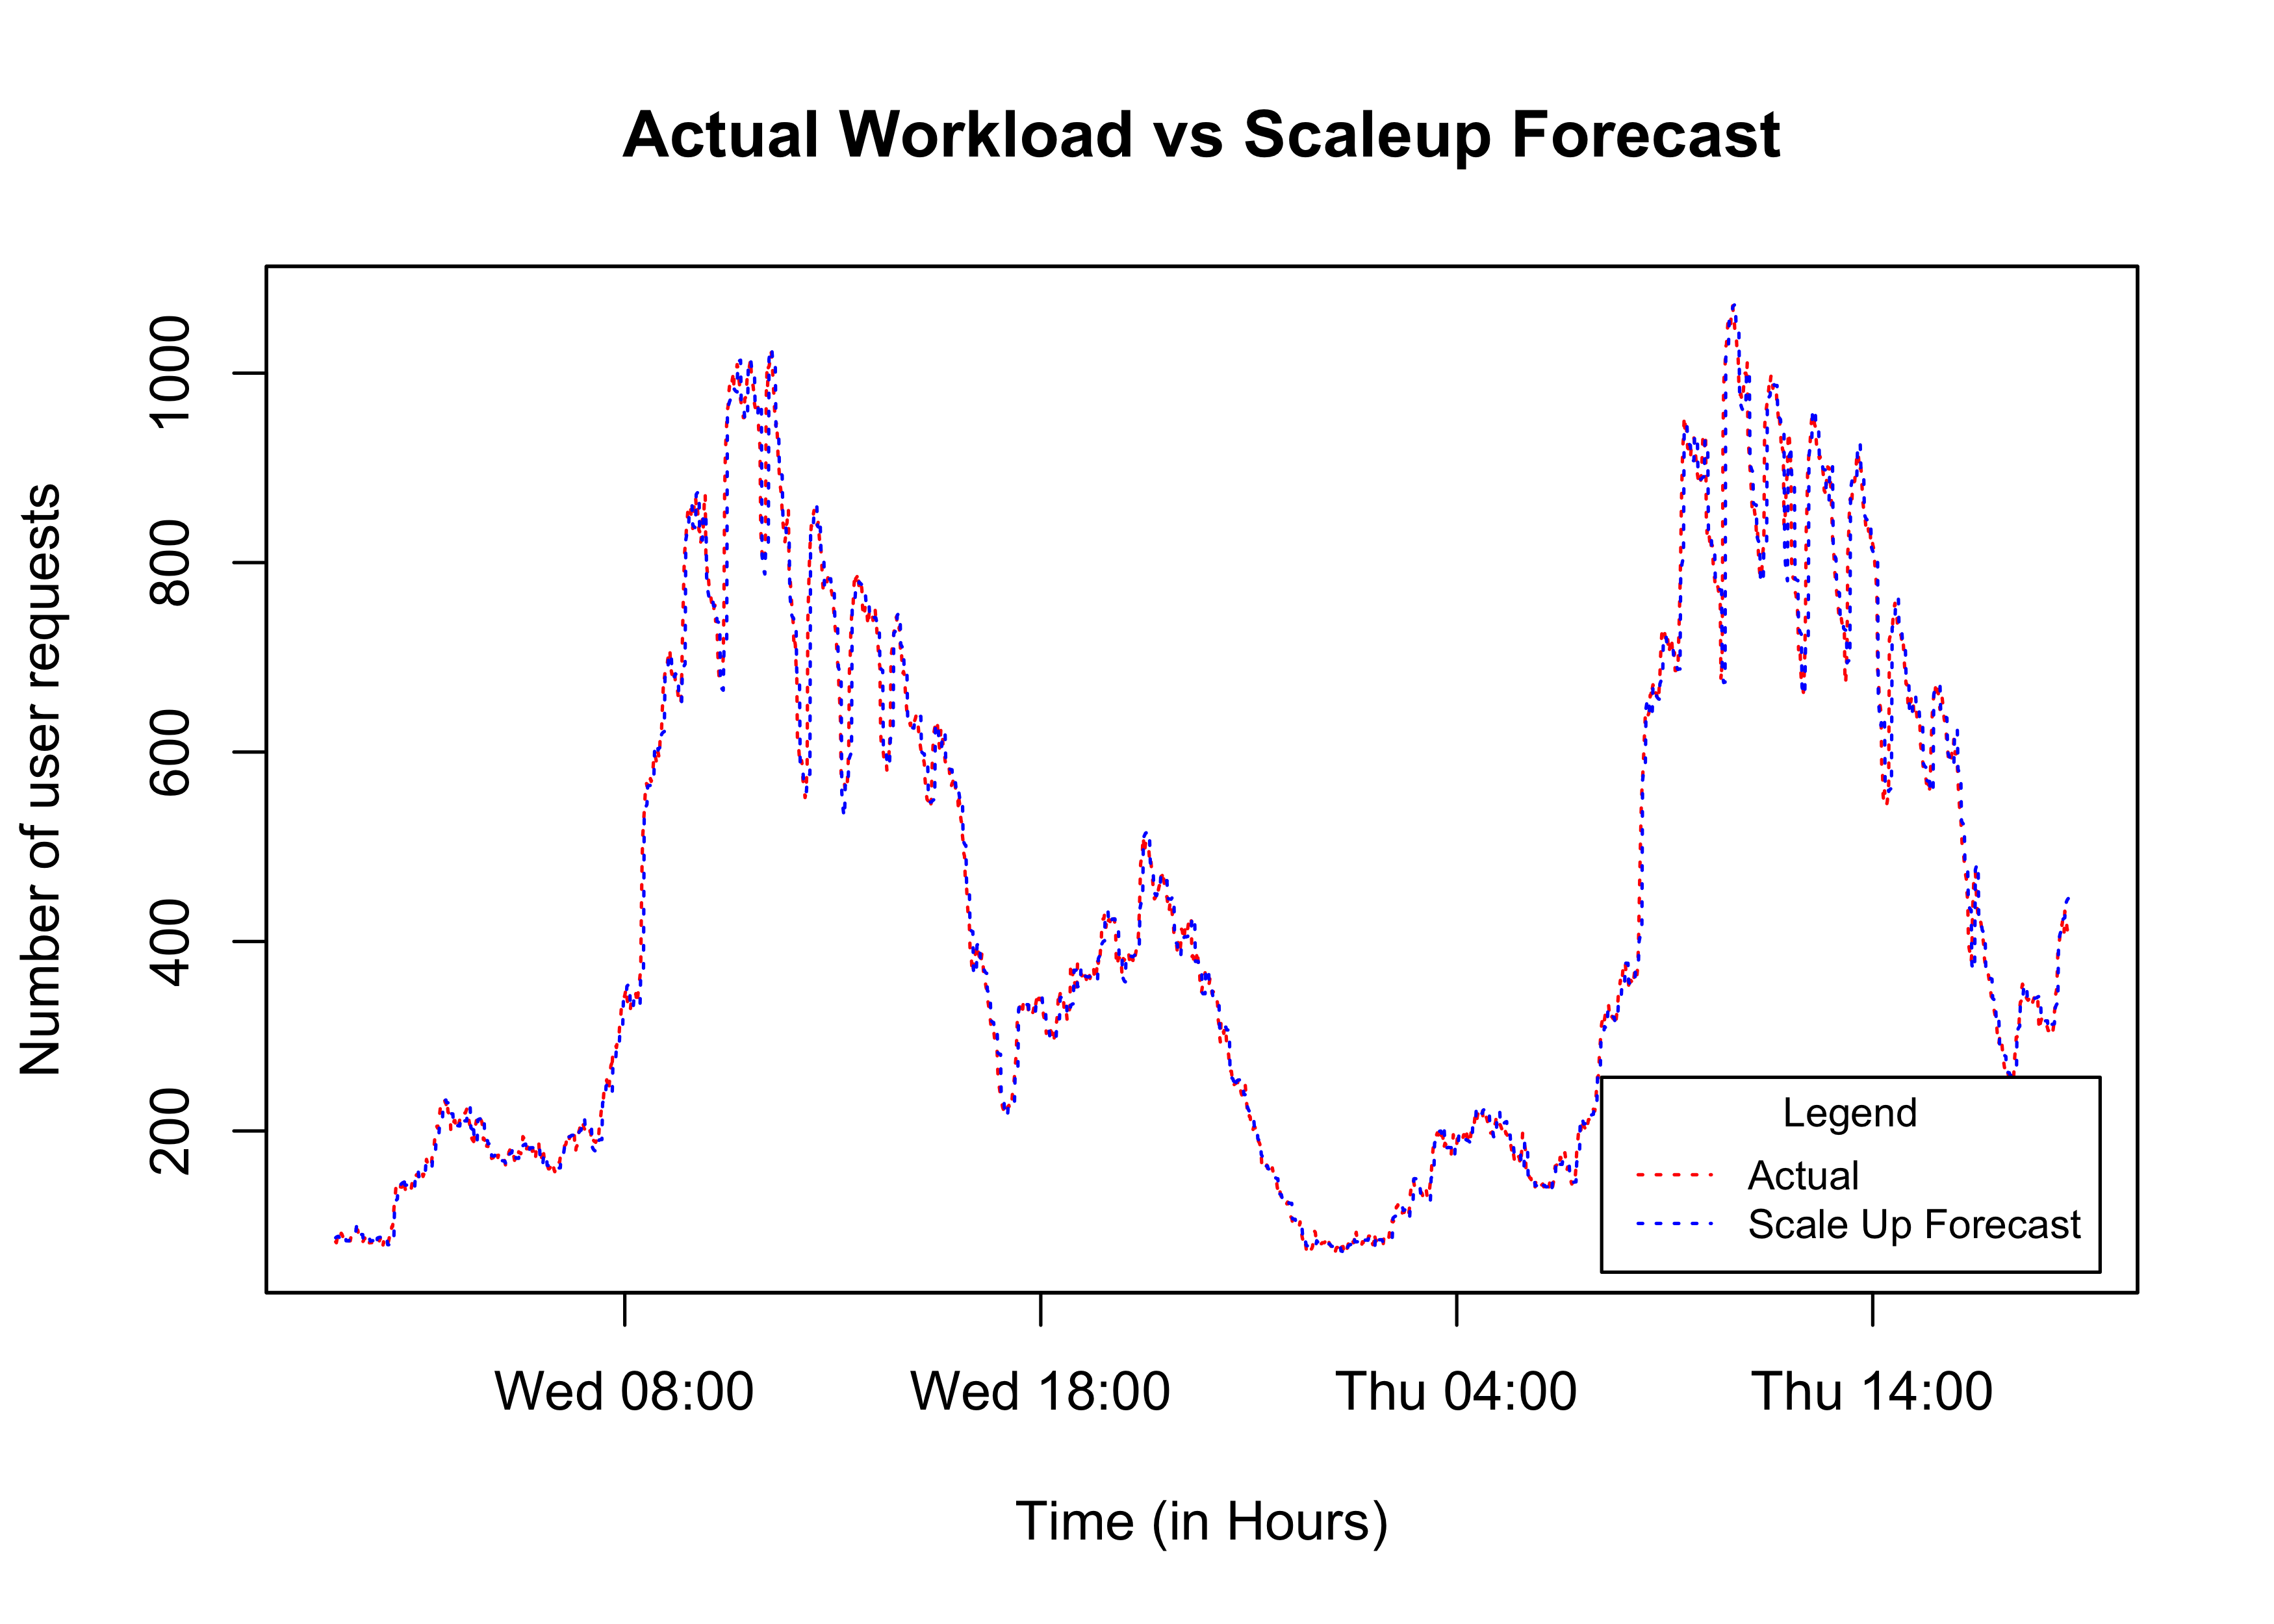
\includegraphics[width=\textwidth]{ScaleUpForecast.png}
         \caption{Scale up forecast}
         \label{figure:forecastscaleup}
     \end{subfigure}
     \begin{subfigure}[b]{0.9\textwidth}
         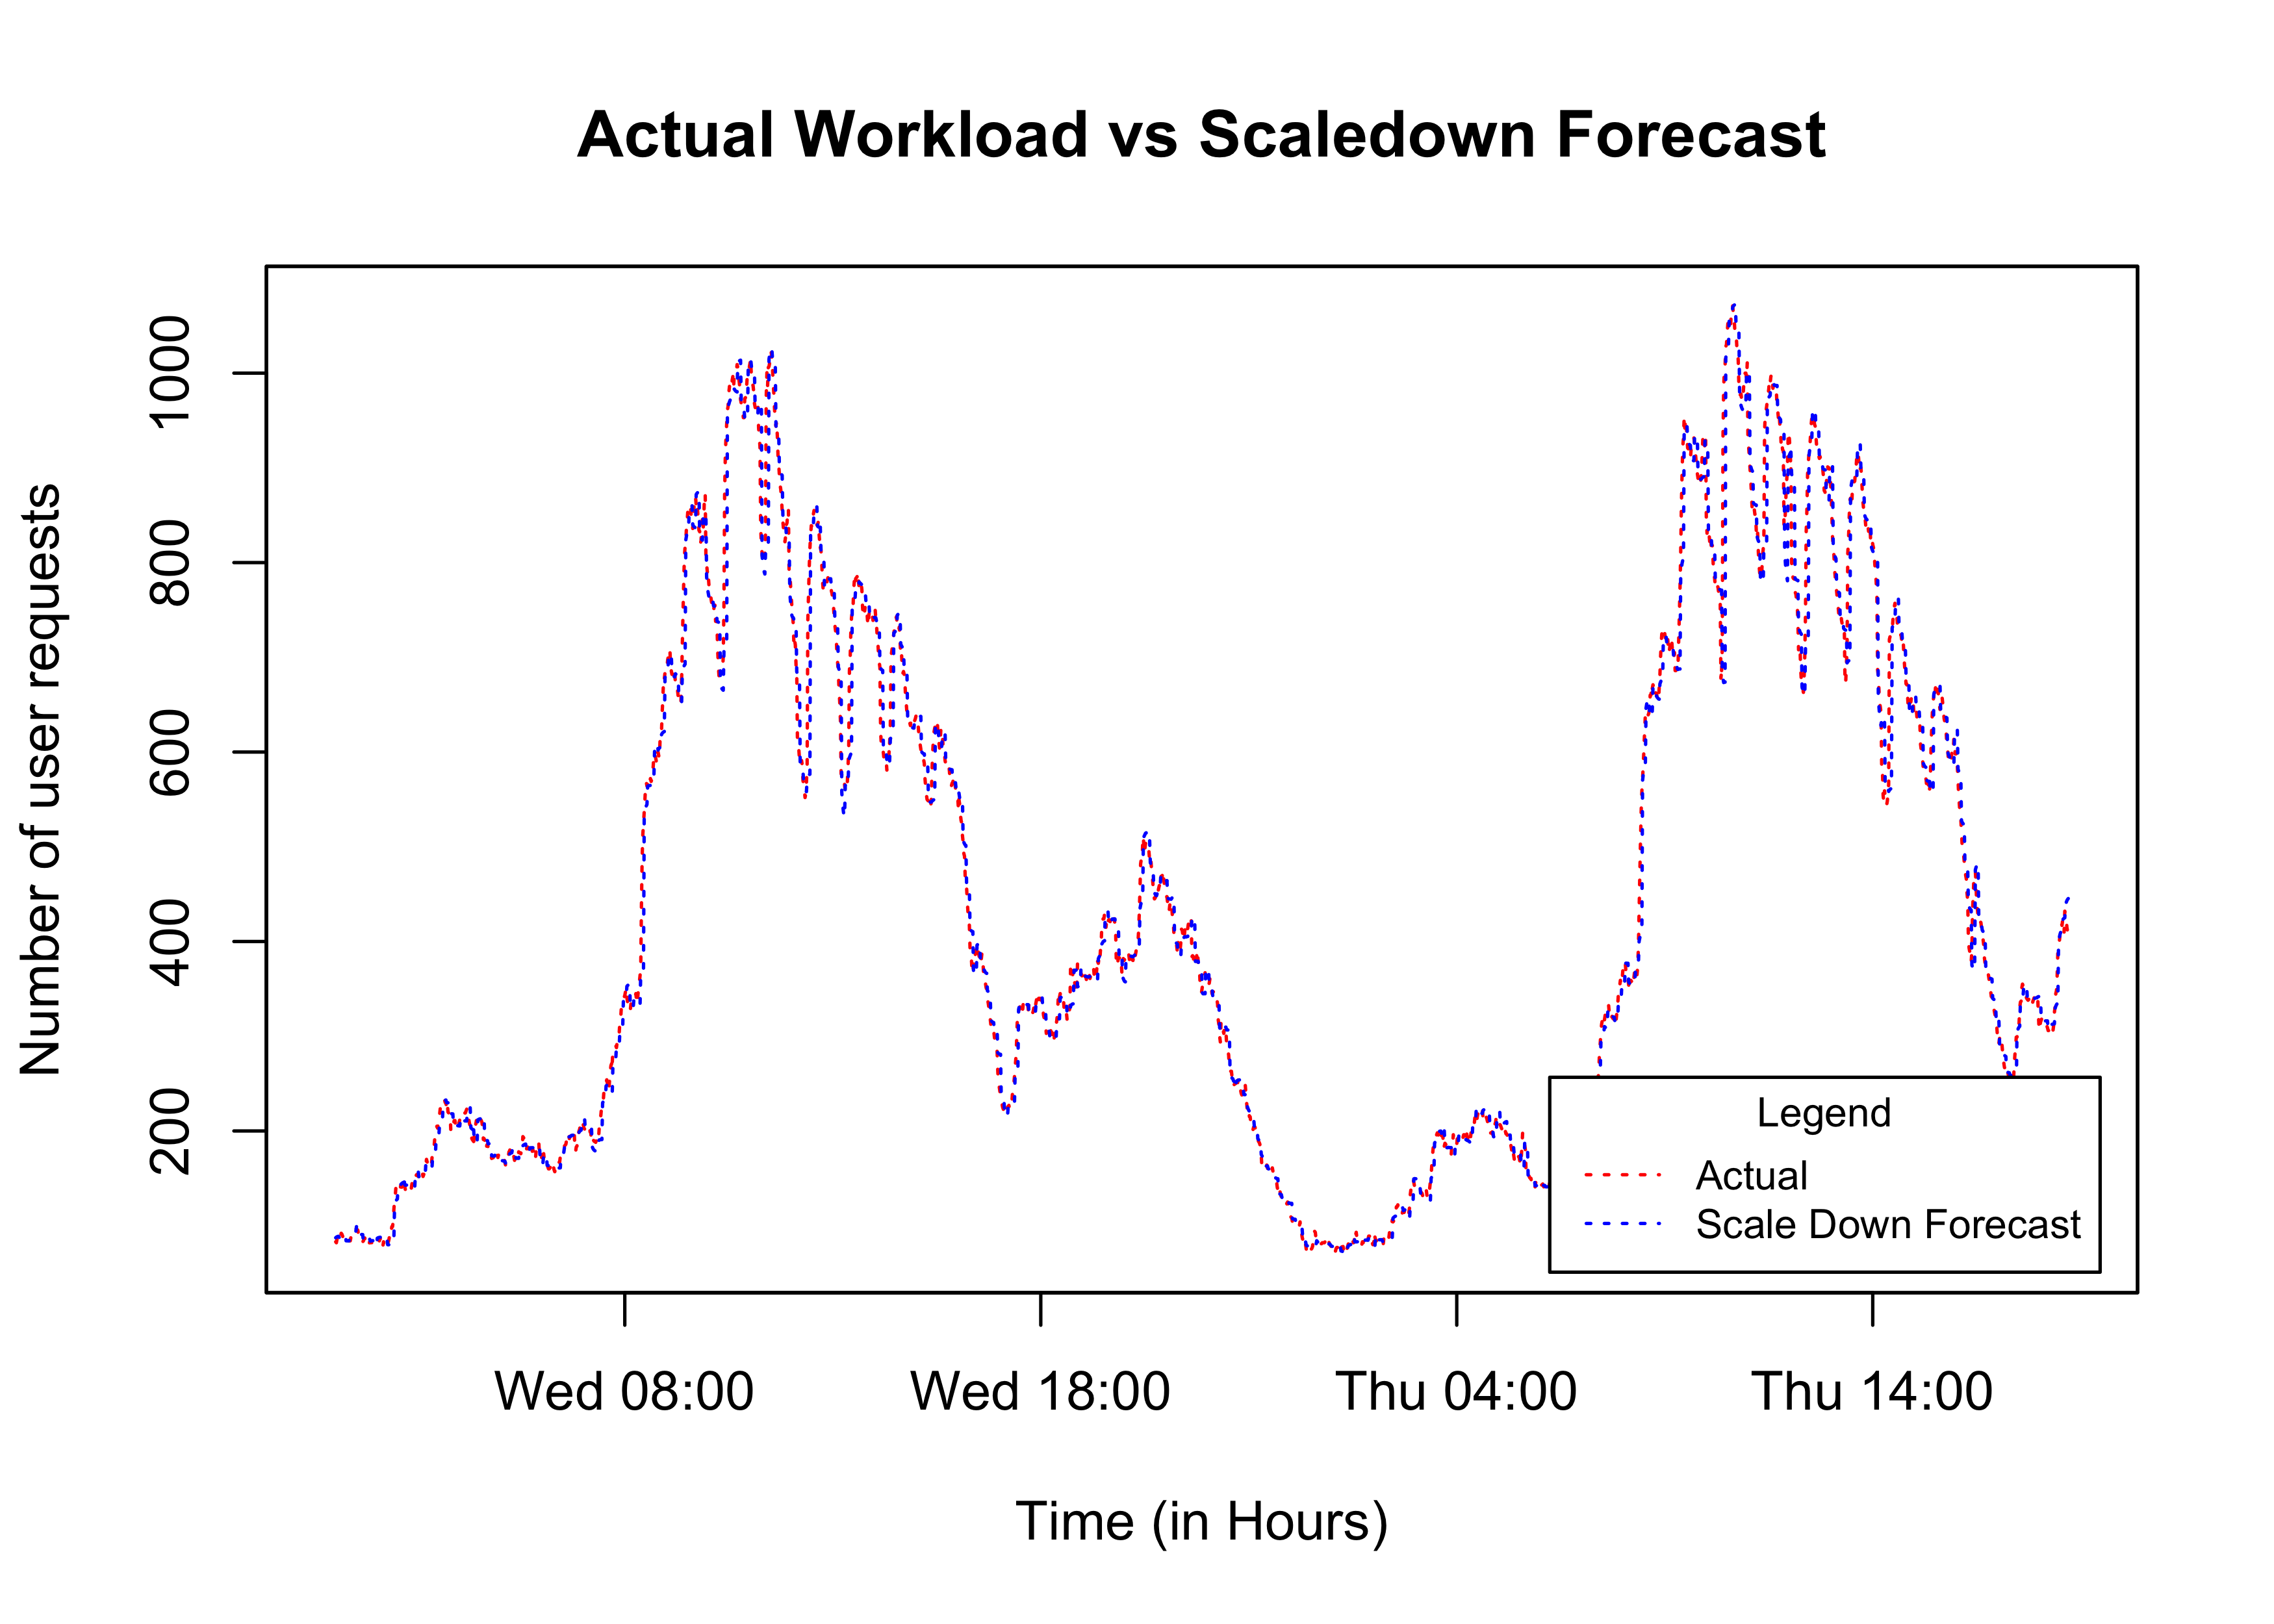
\includegraphics[width=\textwidth]{ScaleDownForecast.png}
         \caption{Scale down forecast}
         \label{figure:forecastscaledown}
     \end{subfigure}
     \caption{Forecast for Scale Up and Down}
     \label{fig:forecast}
\end{figure}
\begin{figure}
     \centering
     \begin{subfigure}[b]{0.45\textwidth}
         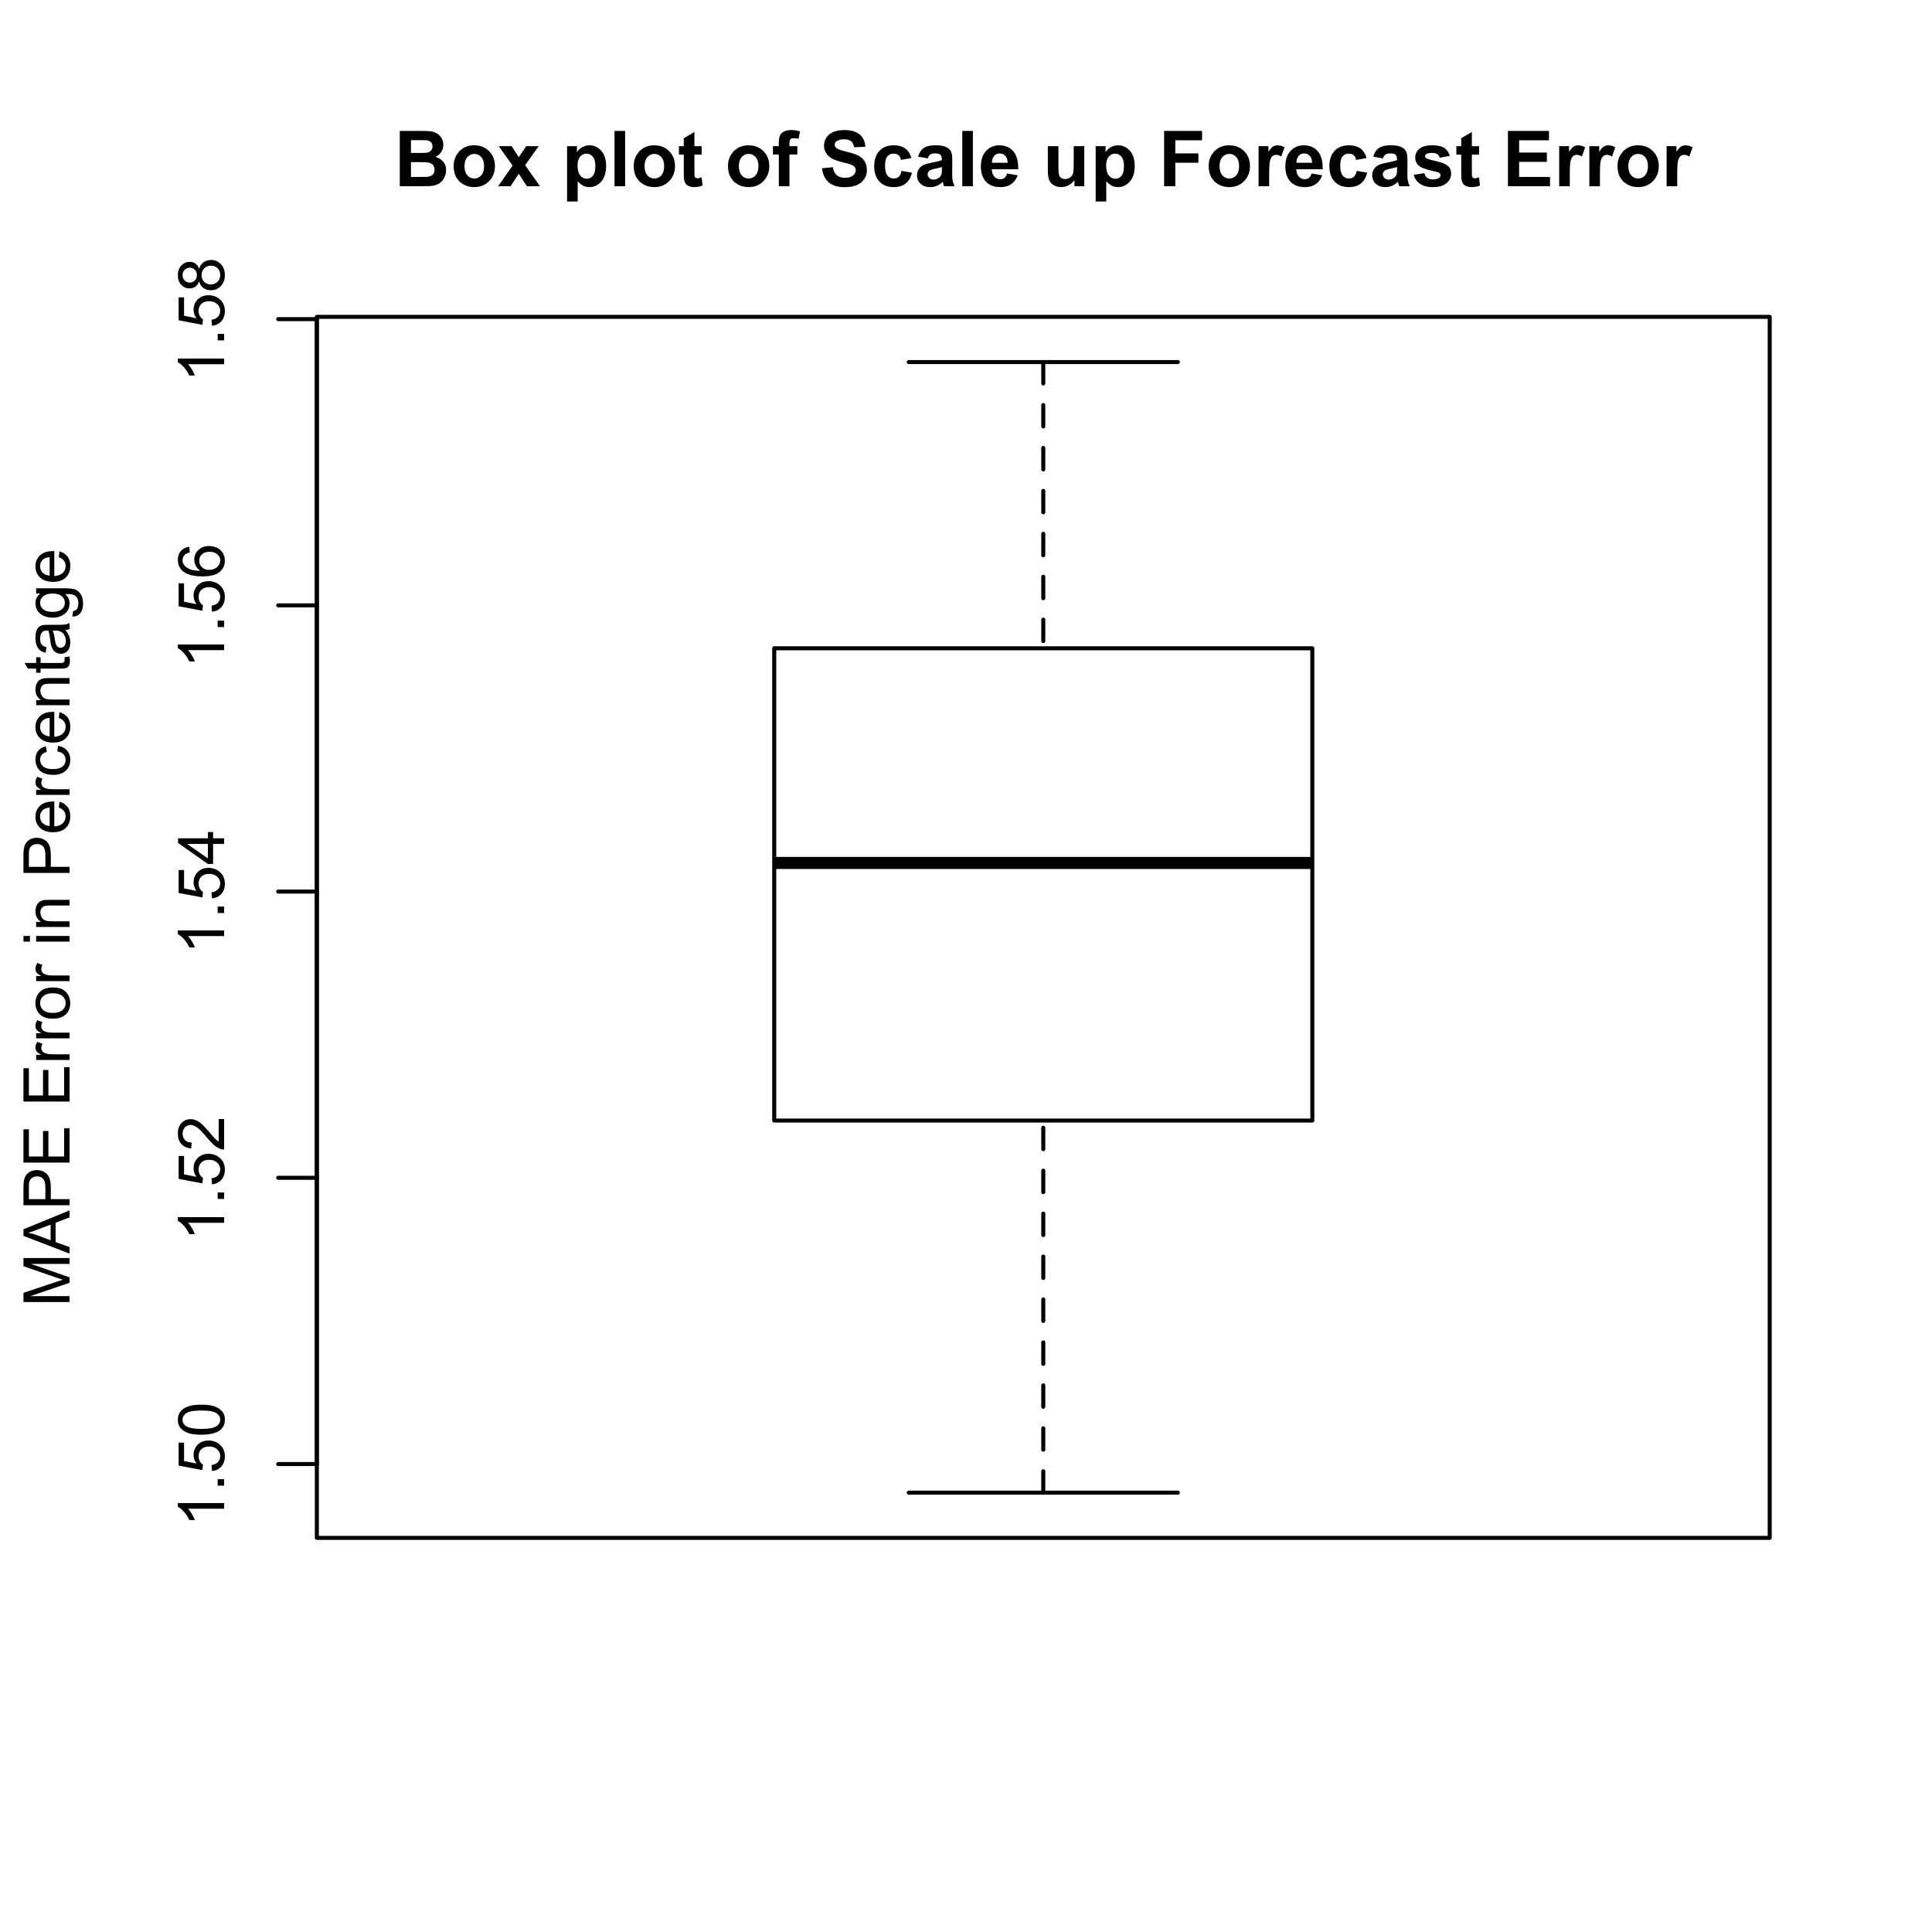
\includegraphics[width=\textwidth]{ScaleUpAcc.png}
         \caption{Scale up forecast error}
         \label{figure:forecastscaleuperror}
     \end{subfigure}
     \hfill
     \begin{subfigure}[b]{0.45\textwidth}
         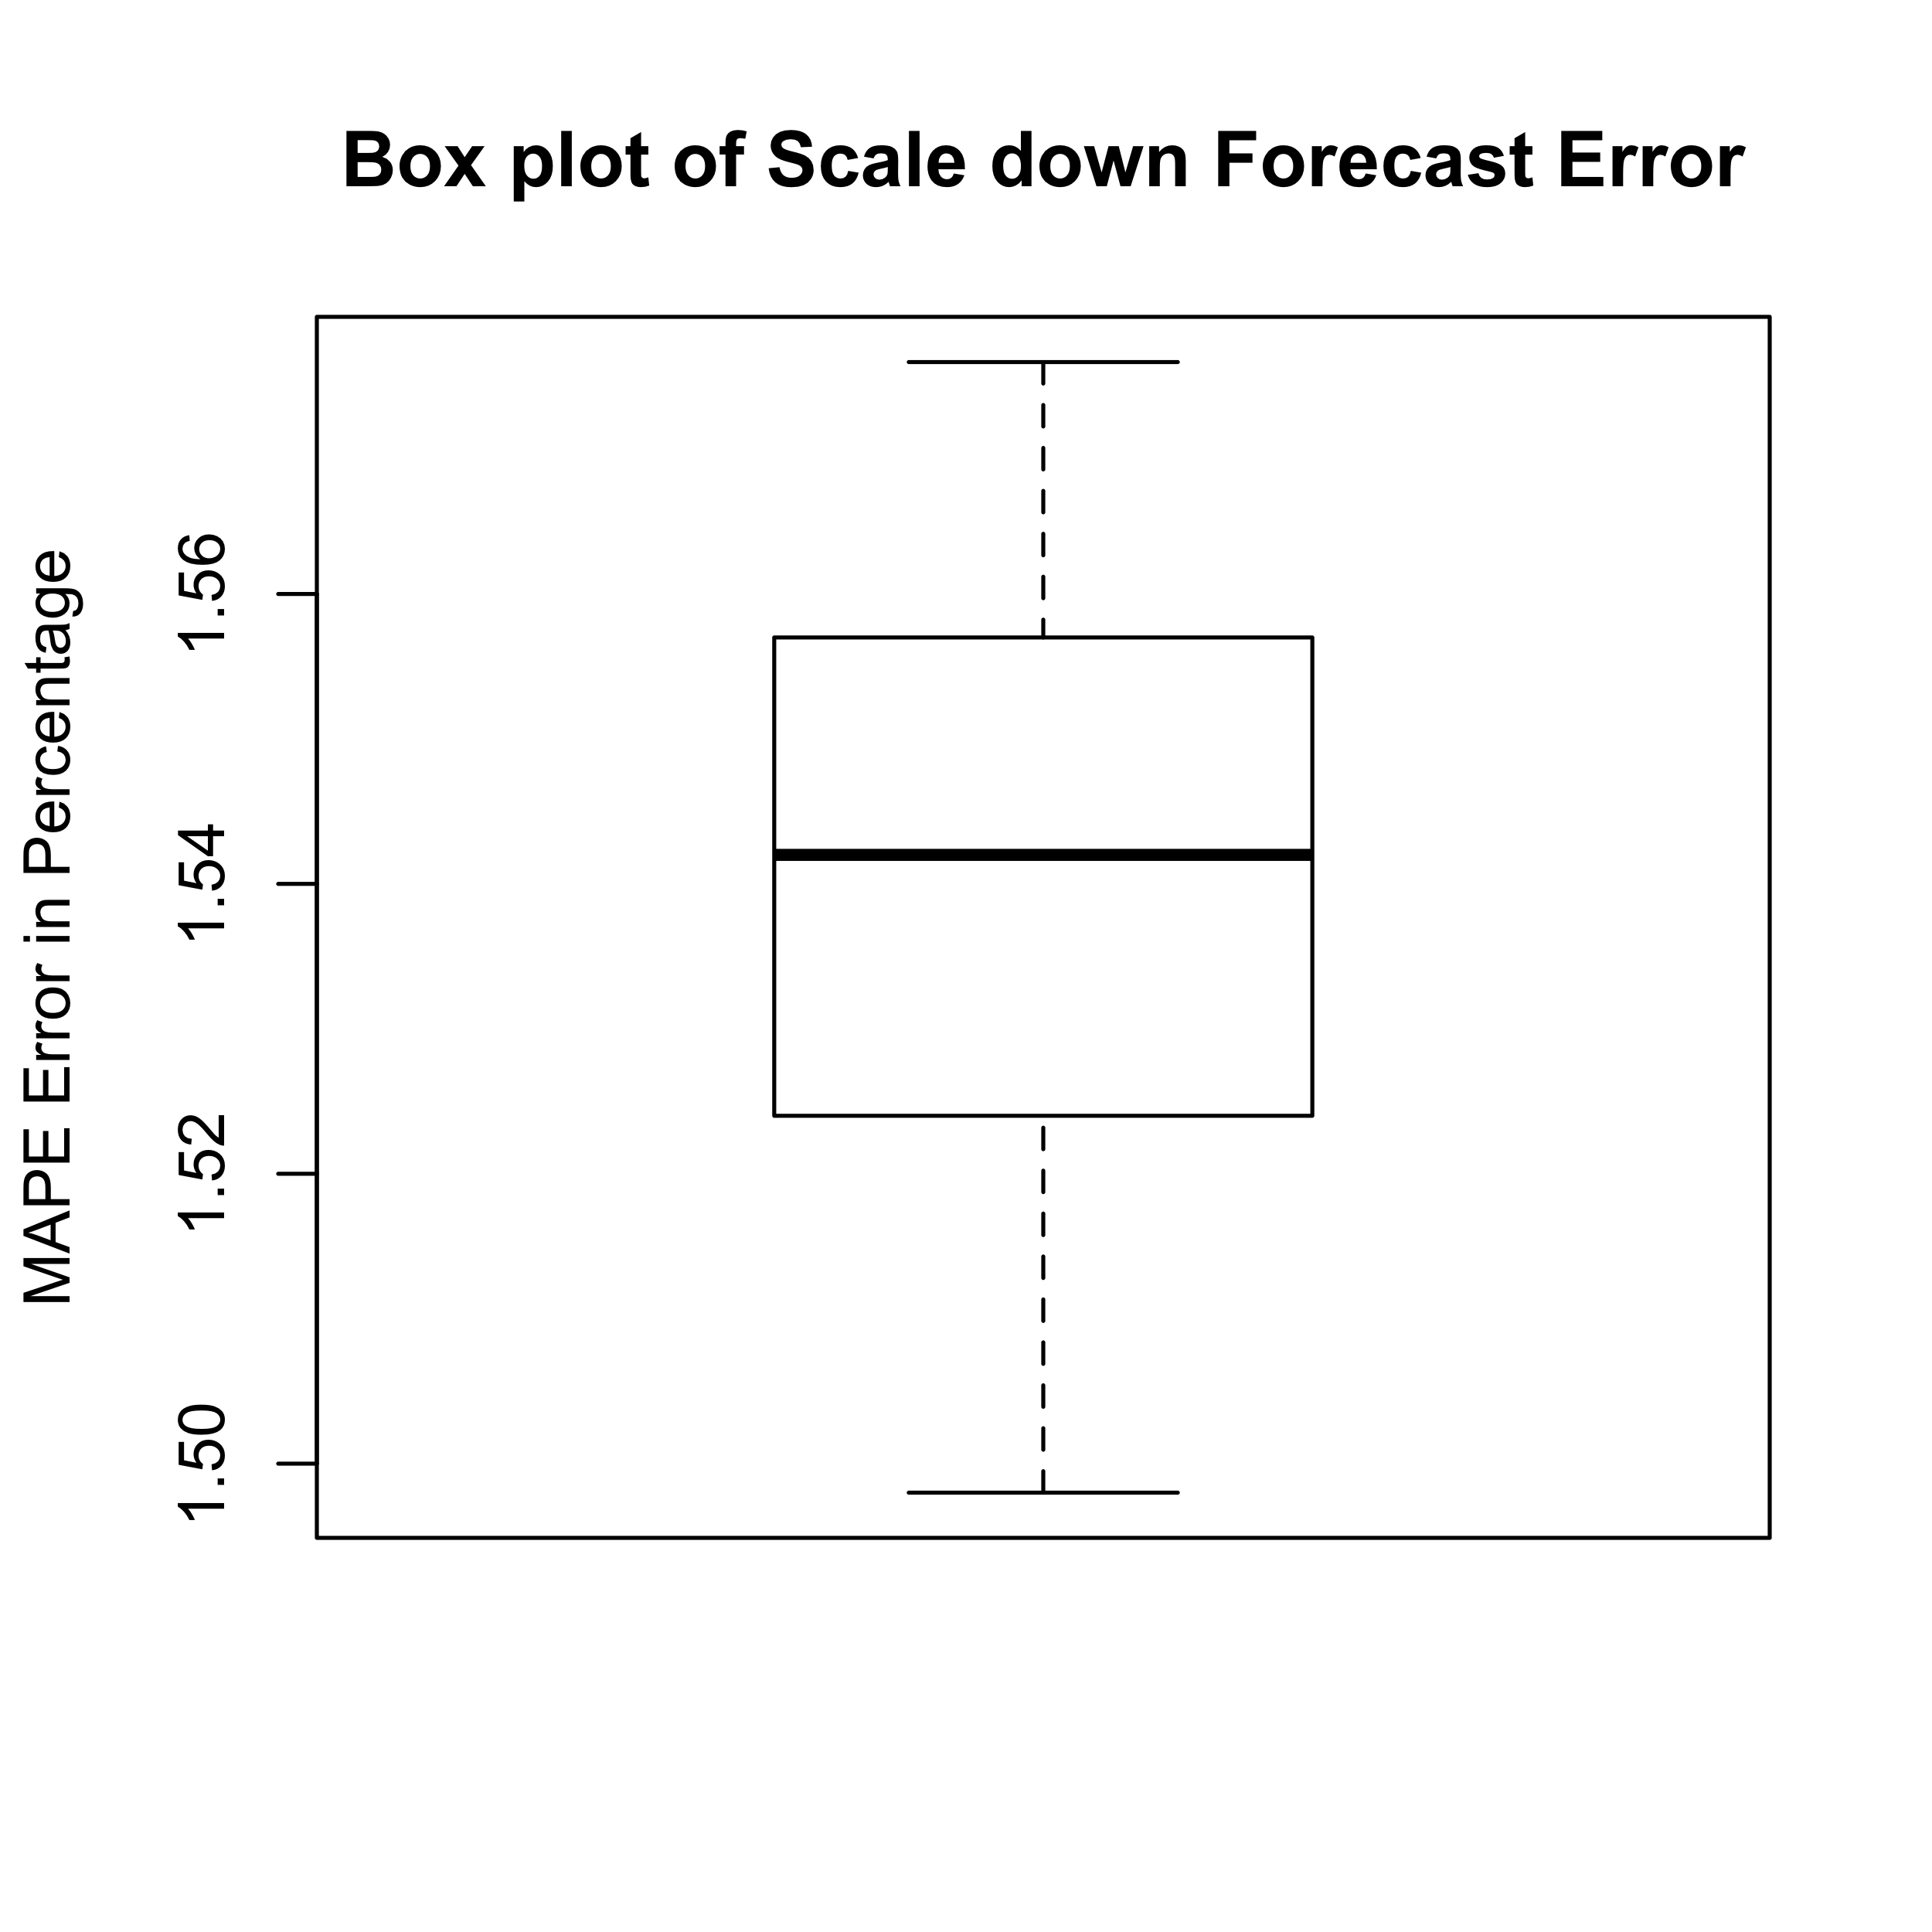
\includegraphics[width=\textwidth]{ScaleDownAcc.png}
         \caption{Scale down forecast error}
         \label{figure:forecastscaledownerror}
     \end{subfigure}
     \caption{Forecast Errors}
     \label{fig:forecasterror}
\end{figure}
\subsection{SLA violation}
\label{sub:SLA violation}
As discussed in previous section, AppElastic algorithm will run on the predicted workloads which is generated by ARIMA model. As it was clear form the previous section, ARIMA model has forecast error of 1.5\% in both scale up and scale down forecasts. These forecast error leads to SLA violations\footnote{Refer section~\ref{sec:SLA Violations}}. Figure~\ref{fig:forecasterror} some examples of SLA violation due to forecast error. Its evident from the Figure~\ref{fig:forecasterror}, the capacity of provisioned VM's falls short to support user request, hence some of the user request falls above the green line. Equation~\ref{eq:userslavio} is used to calculate how many of these users face SLA violation and have degraded quality of services or no service. As show in the case analysis~\ref{eq:slaviocase}, SLA violation will occur when the required number of VM's to fulfill user requests is more than number of VM's active. These SLA violation is evident from the experiments conducted and the graphs related to these SLA violations are in Figure~\ref{fig:slaviolationgraphs}. As its show in the Figure~\ref{figure:slaviolation1} and Figure~\ref{figure:slaviolation2}, number of VM's active in some parts of the graph are less than the number of user requests arriving to the system. Figure~\ref{figure:boxplotslaviolation} the boxplot of number of users for which SLA is violated. Based on the experiments up to 168 users has faced SLA violation. To mitigate this problem of SLA violation, the AppElastic algorithm can be further extended to provision more machines in case of rapid increase in workloads. In this case, if AppElastic is configured to provision two more machines which can accommodate 240 users, SLA violation can be totally solved.
\begin{equation}
\textrm{ Identify SLA Violations }=
  \begin{cases}
    VM_{required} - VM_{active} < 0 \textrm{ No SLA violation}\\
    VM_{required} - VM_{active} = 0 \textrm{ No SLA violation}\\
    VM_{required} - VM_{active} > 1 \textrm{ SLA violation}\\
\end{cases}
\label{eq:slaviocase}
\end{equation}
\begin{equation}
Users_{\textrm{SLA violation}} = UserRequest_{t} - Capaticy_{t}
\label{eq:userslavio}
\end{equation}
\begin{figure}
     \centering
     \begin{subfigure}[b]{0.45\textwidth}
         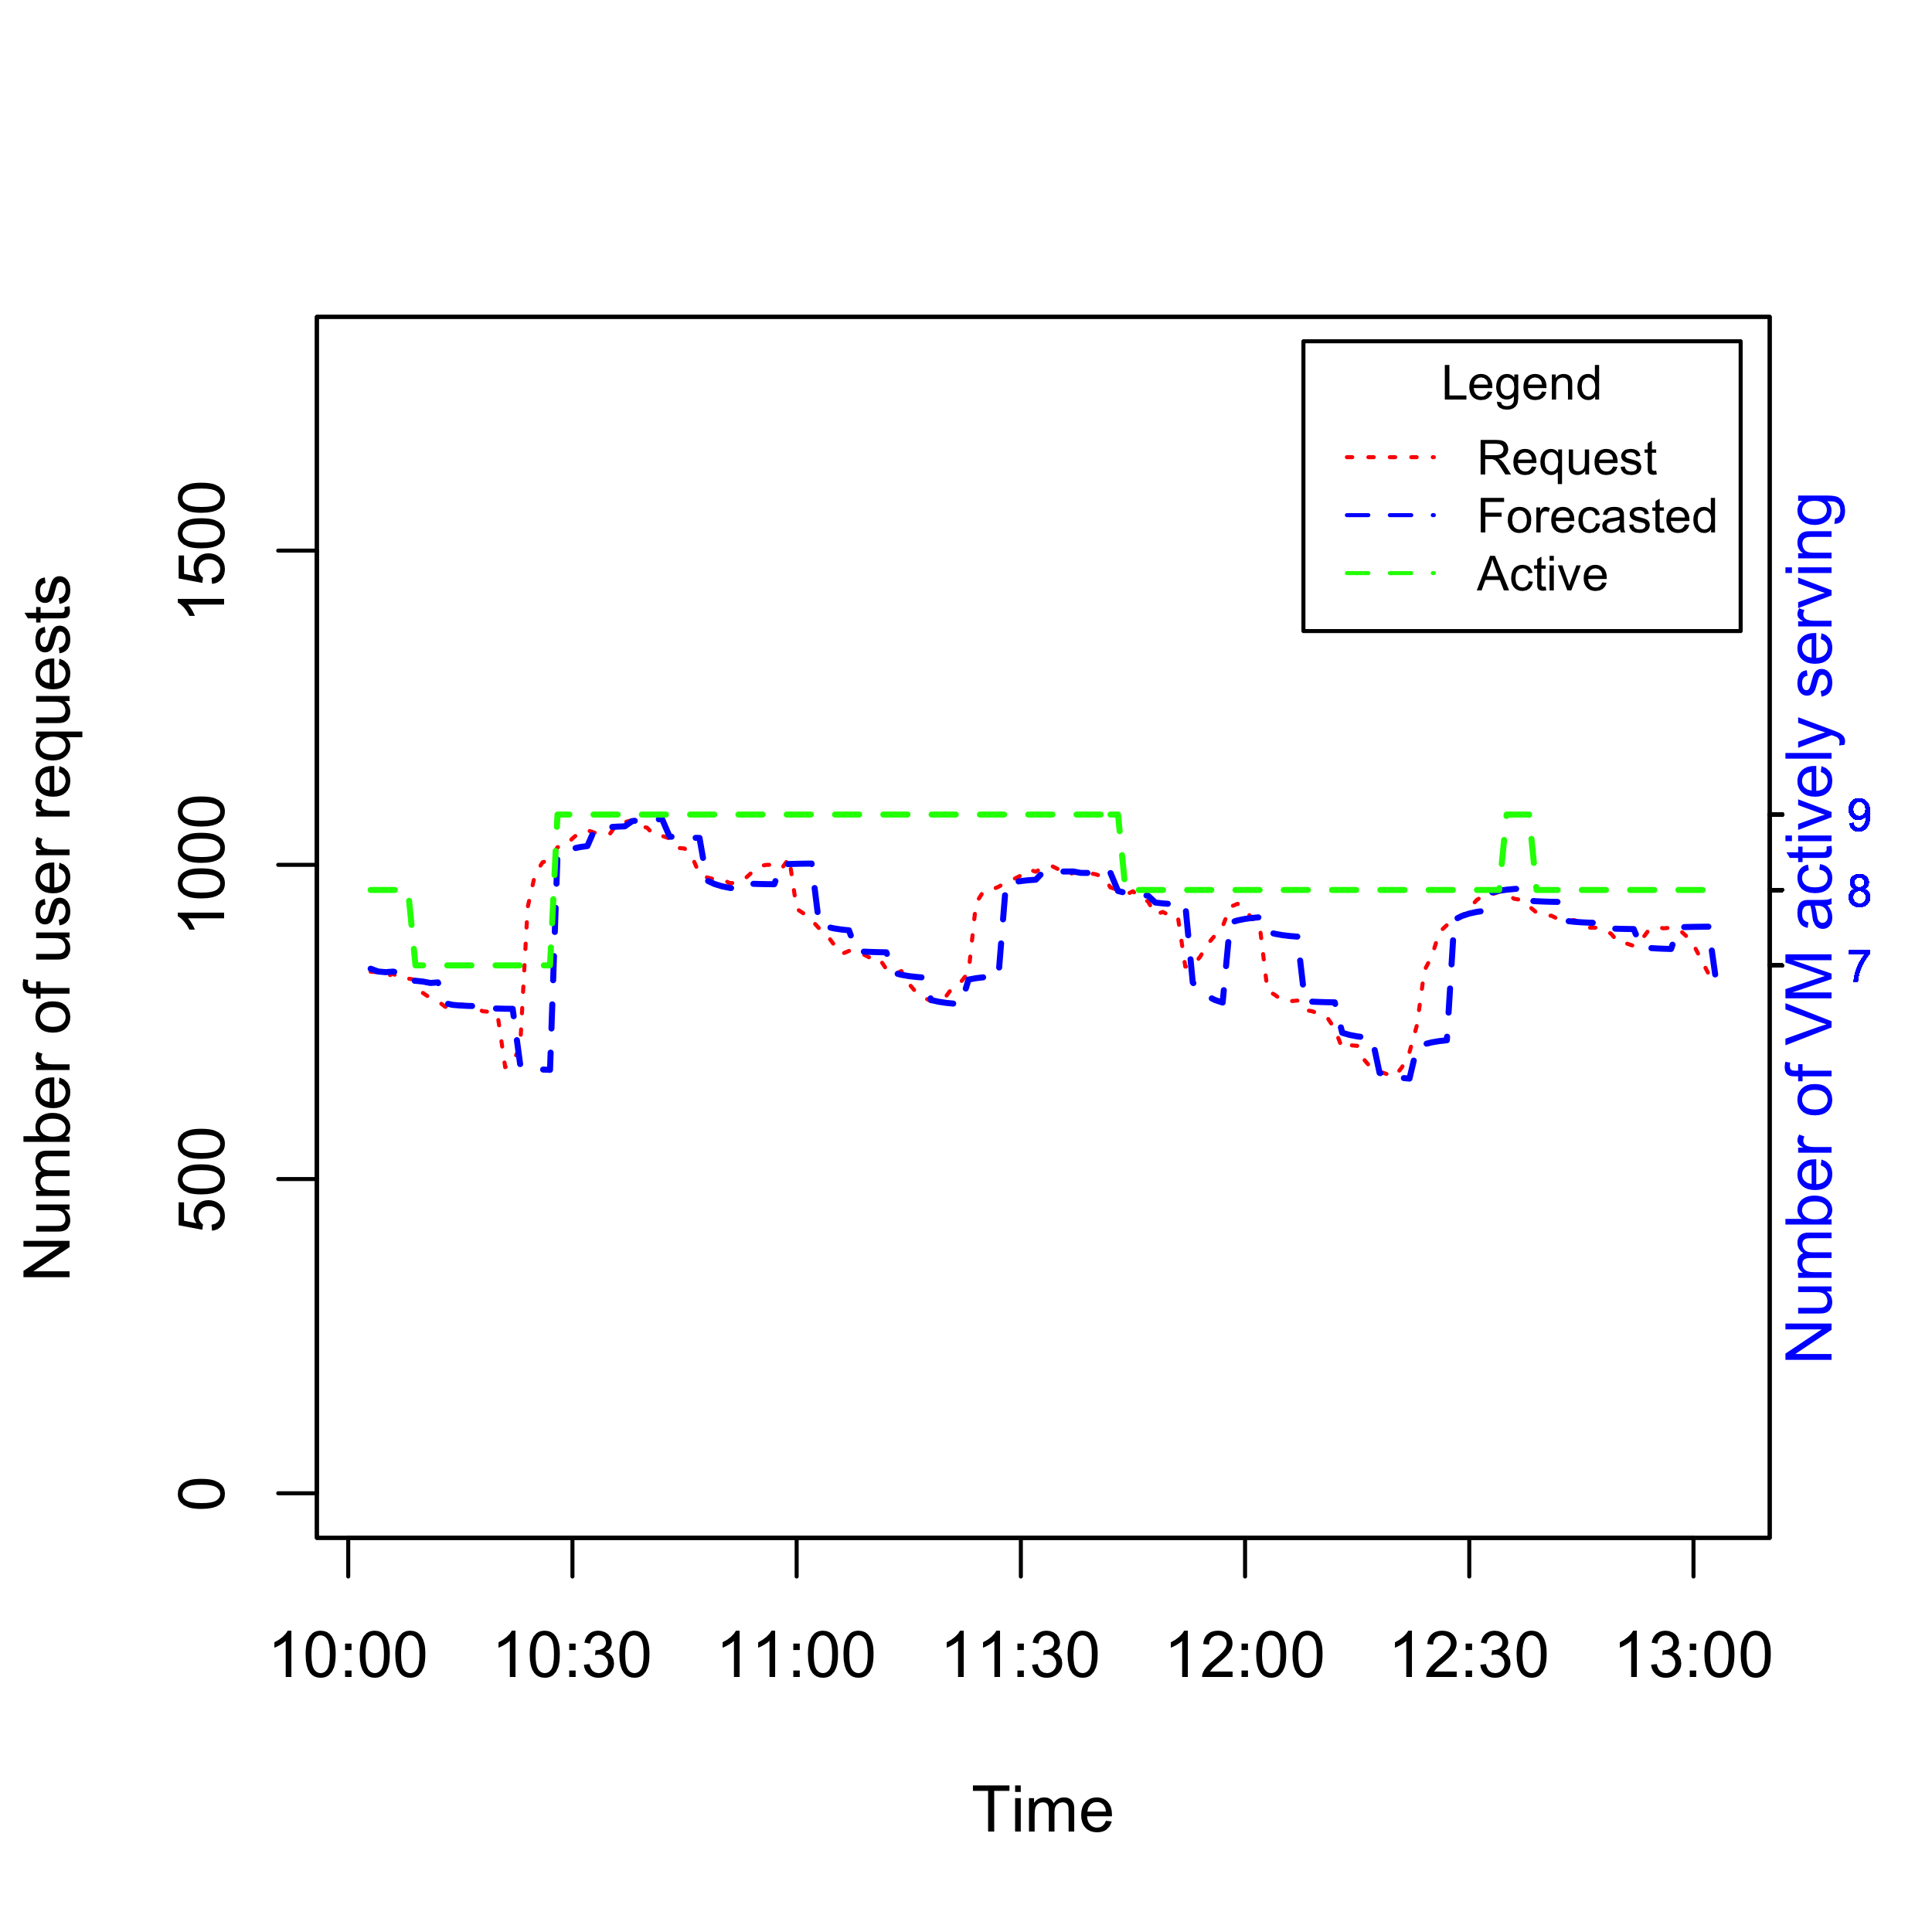
\includegraphics[width=\textwidth]{slaviolation1.png}
         \caption{Example of SLA violation-1}
         \label{figure:slaviolation1}
     \end{subfigure}
     \hfill
     \begin{subfigure}[b]{0.45\textwidth}
         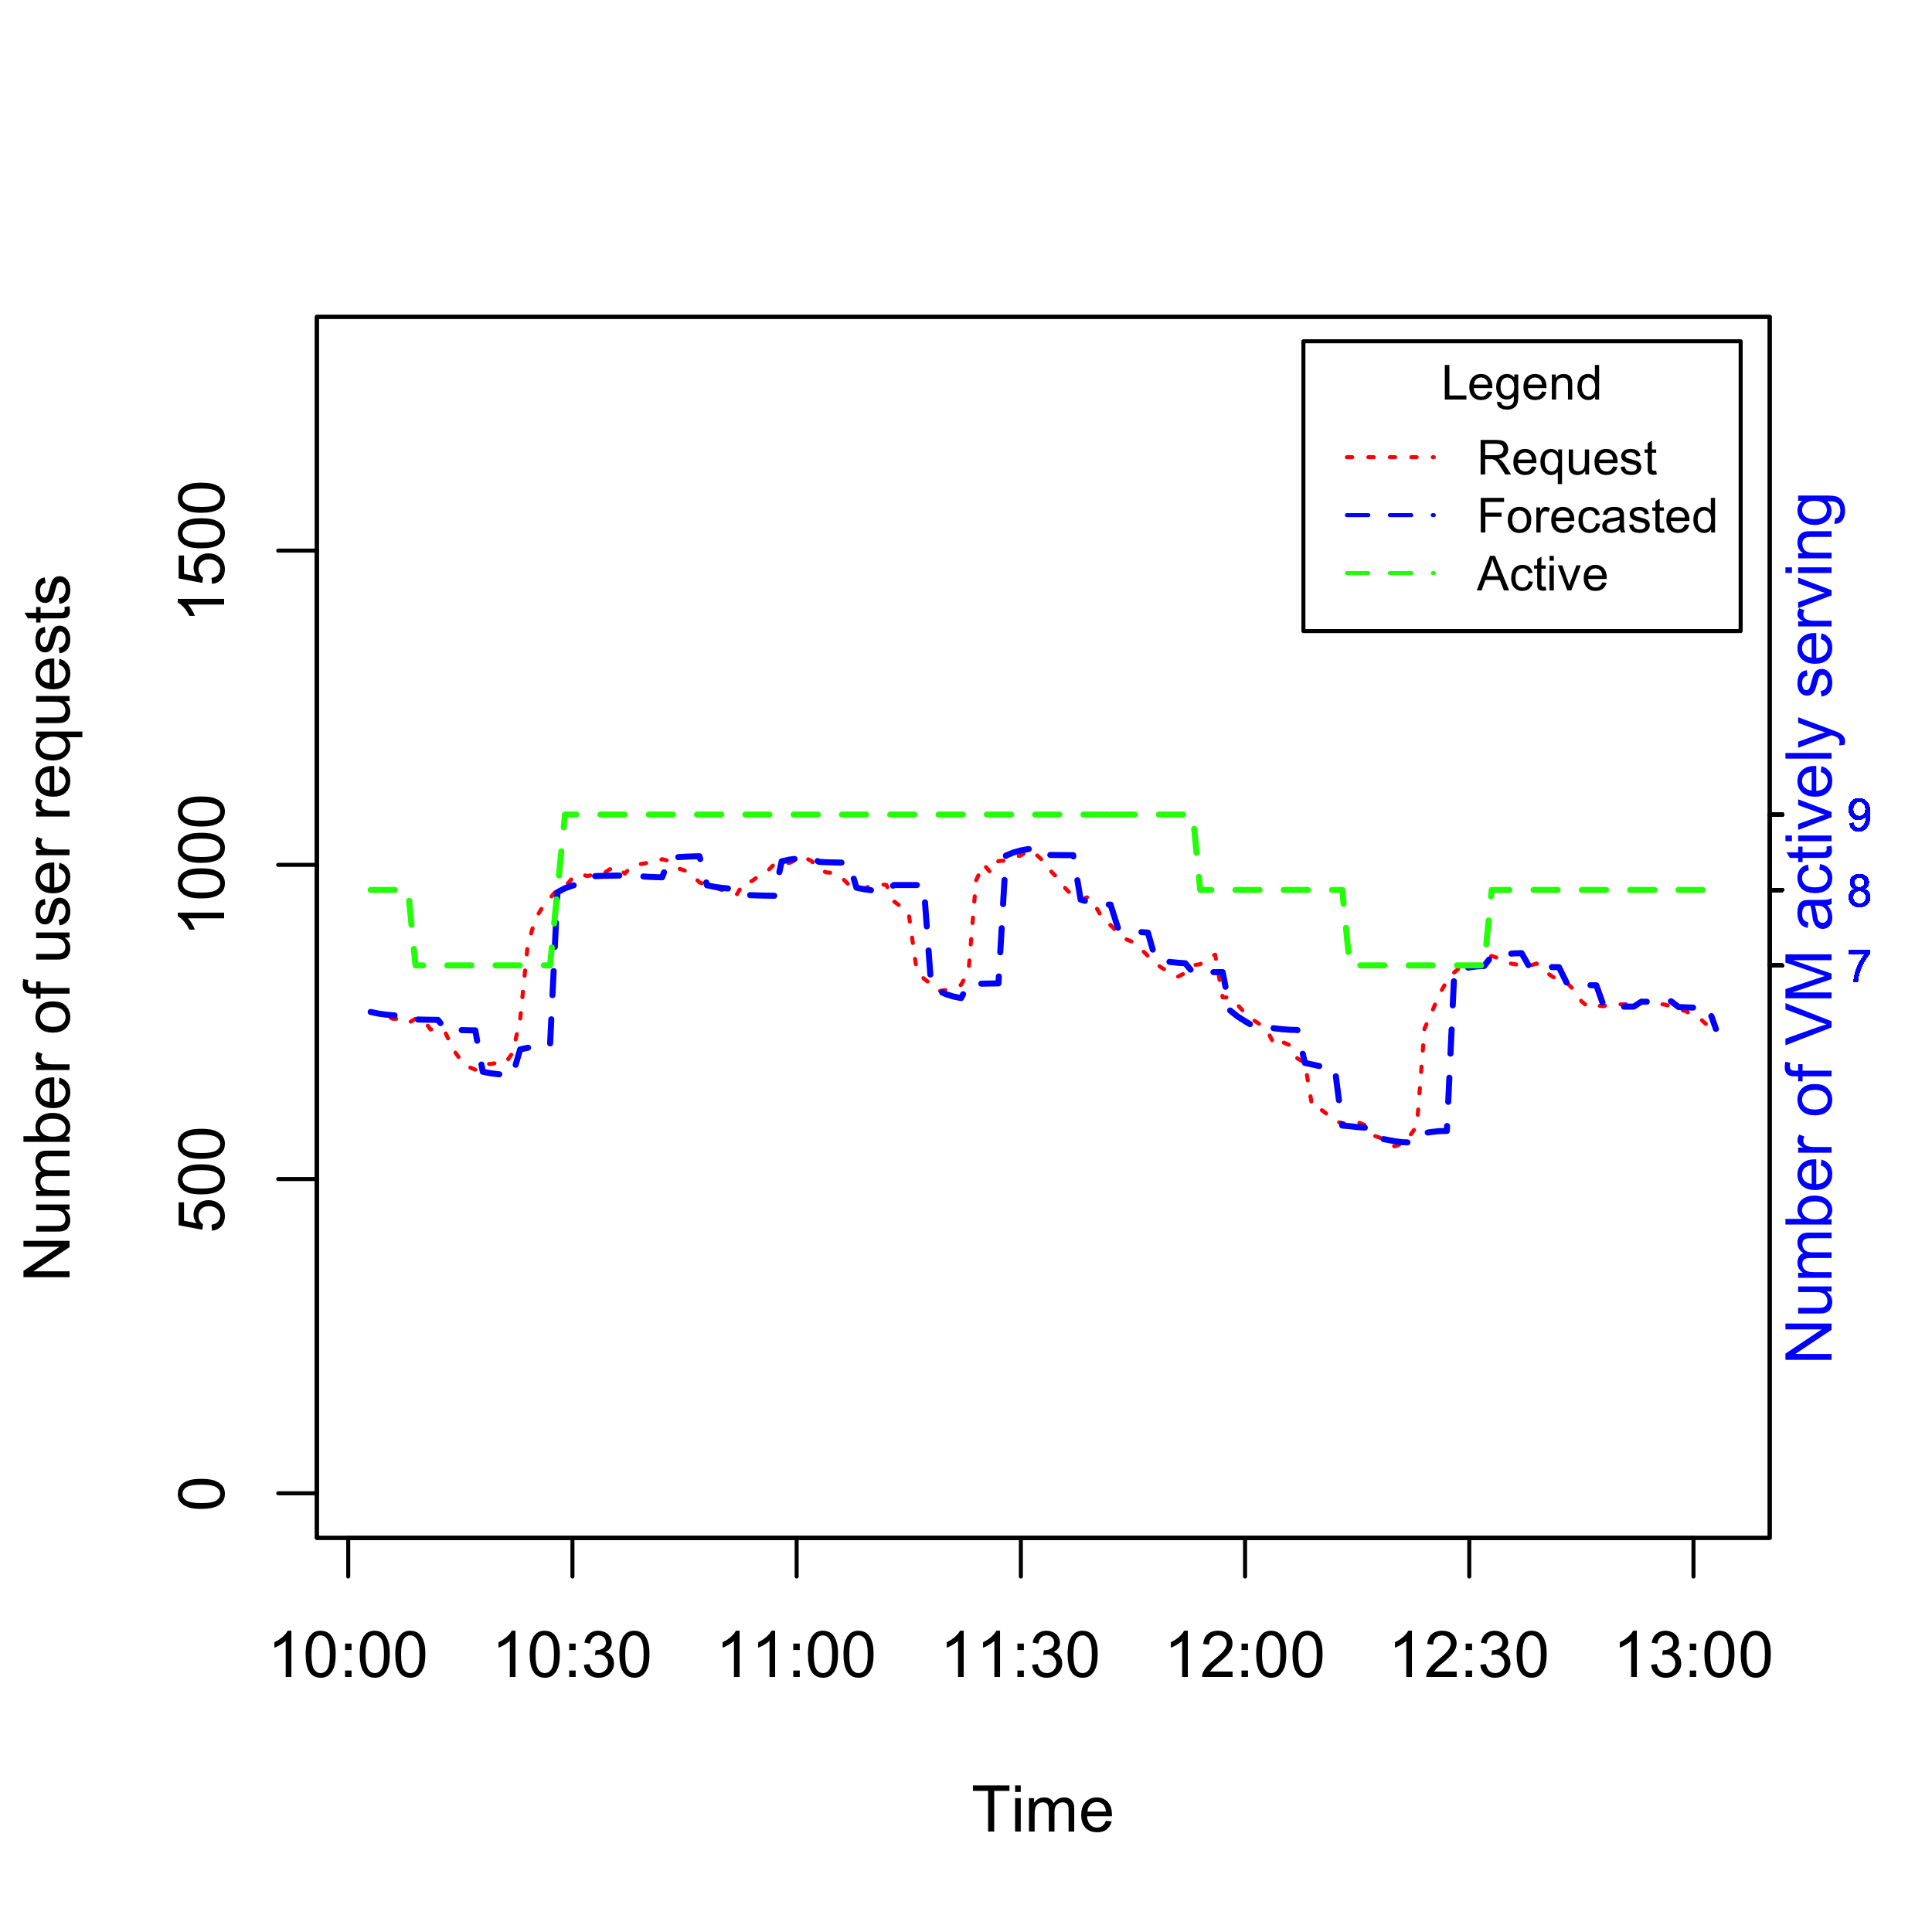
\includegraphics[width=\textwidth]{slaviolation2.png}
         \caption{Example of SLA violation-2}
         \label{figure:slaviolation2}
     \end{subfigure}
     \caption{SLA violation}
     \label{fig:slaviolationgraphs}
\end{figure}

\begin{figure}[h]
  \begin{center}
    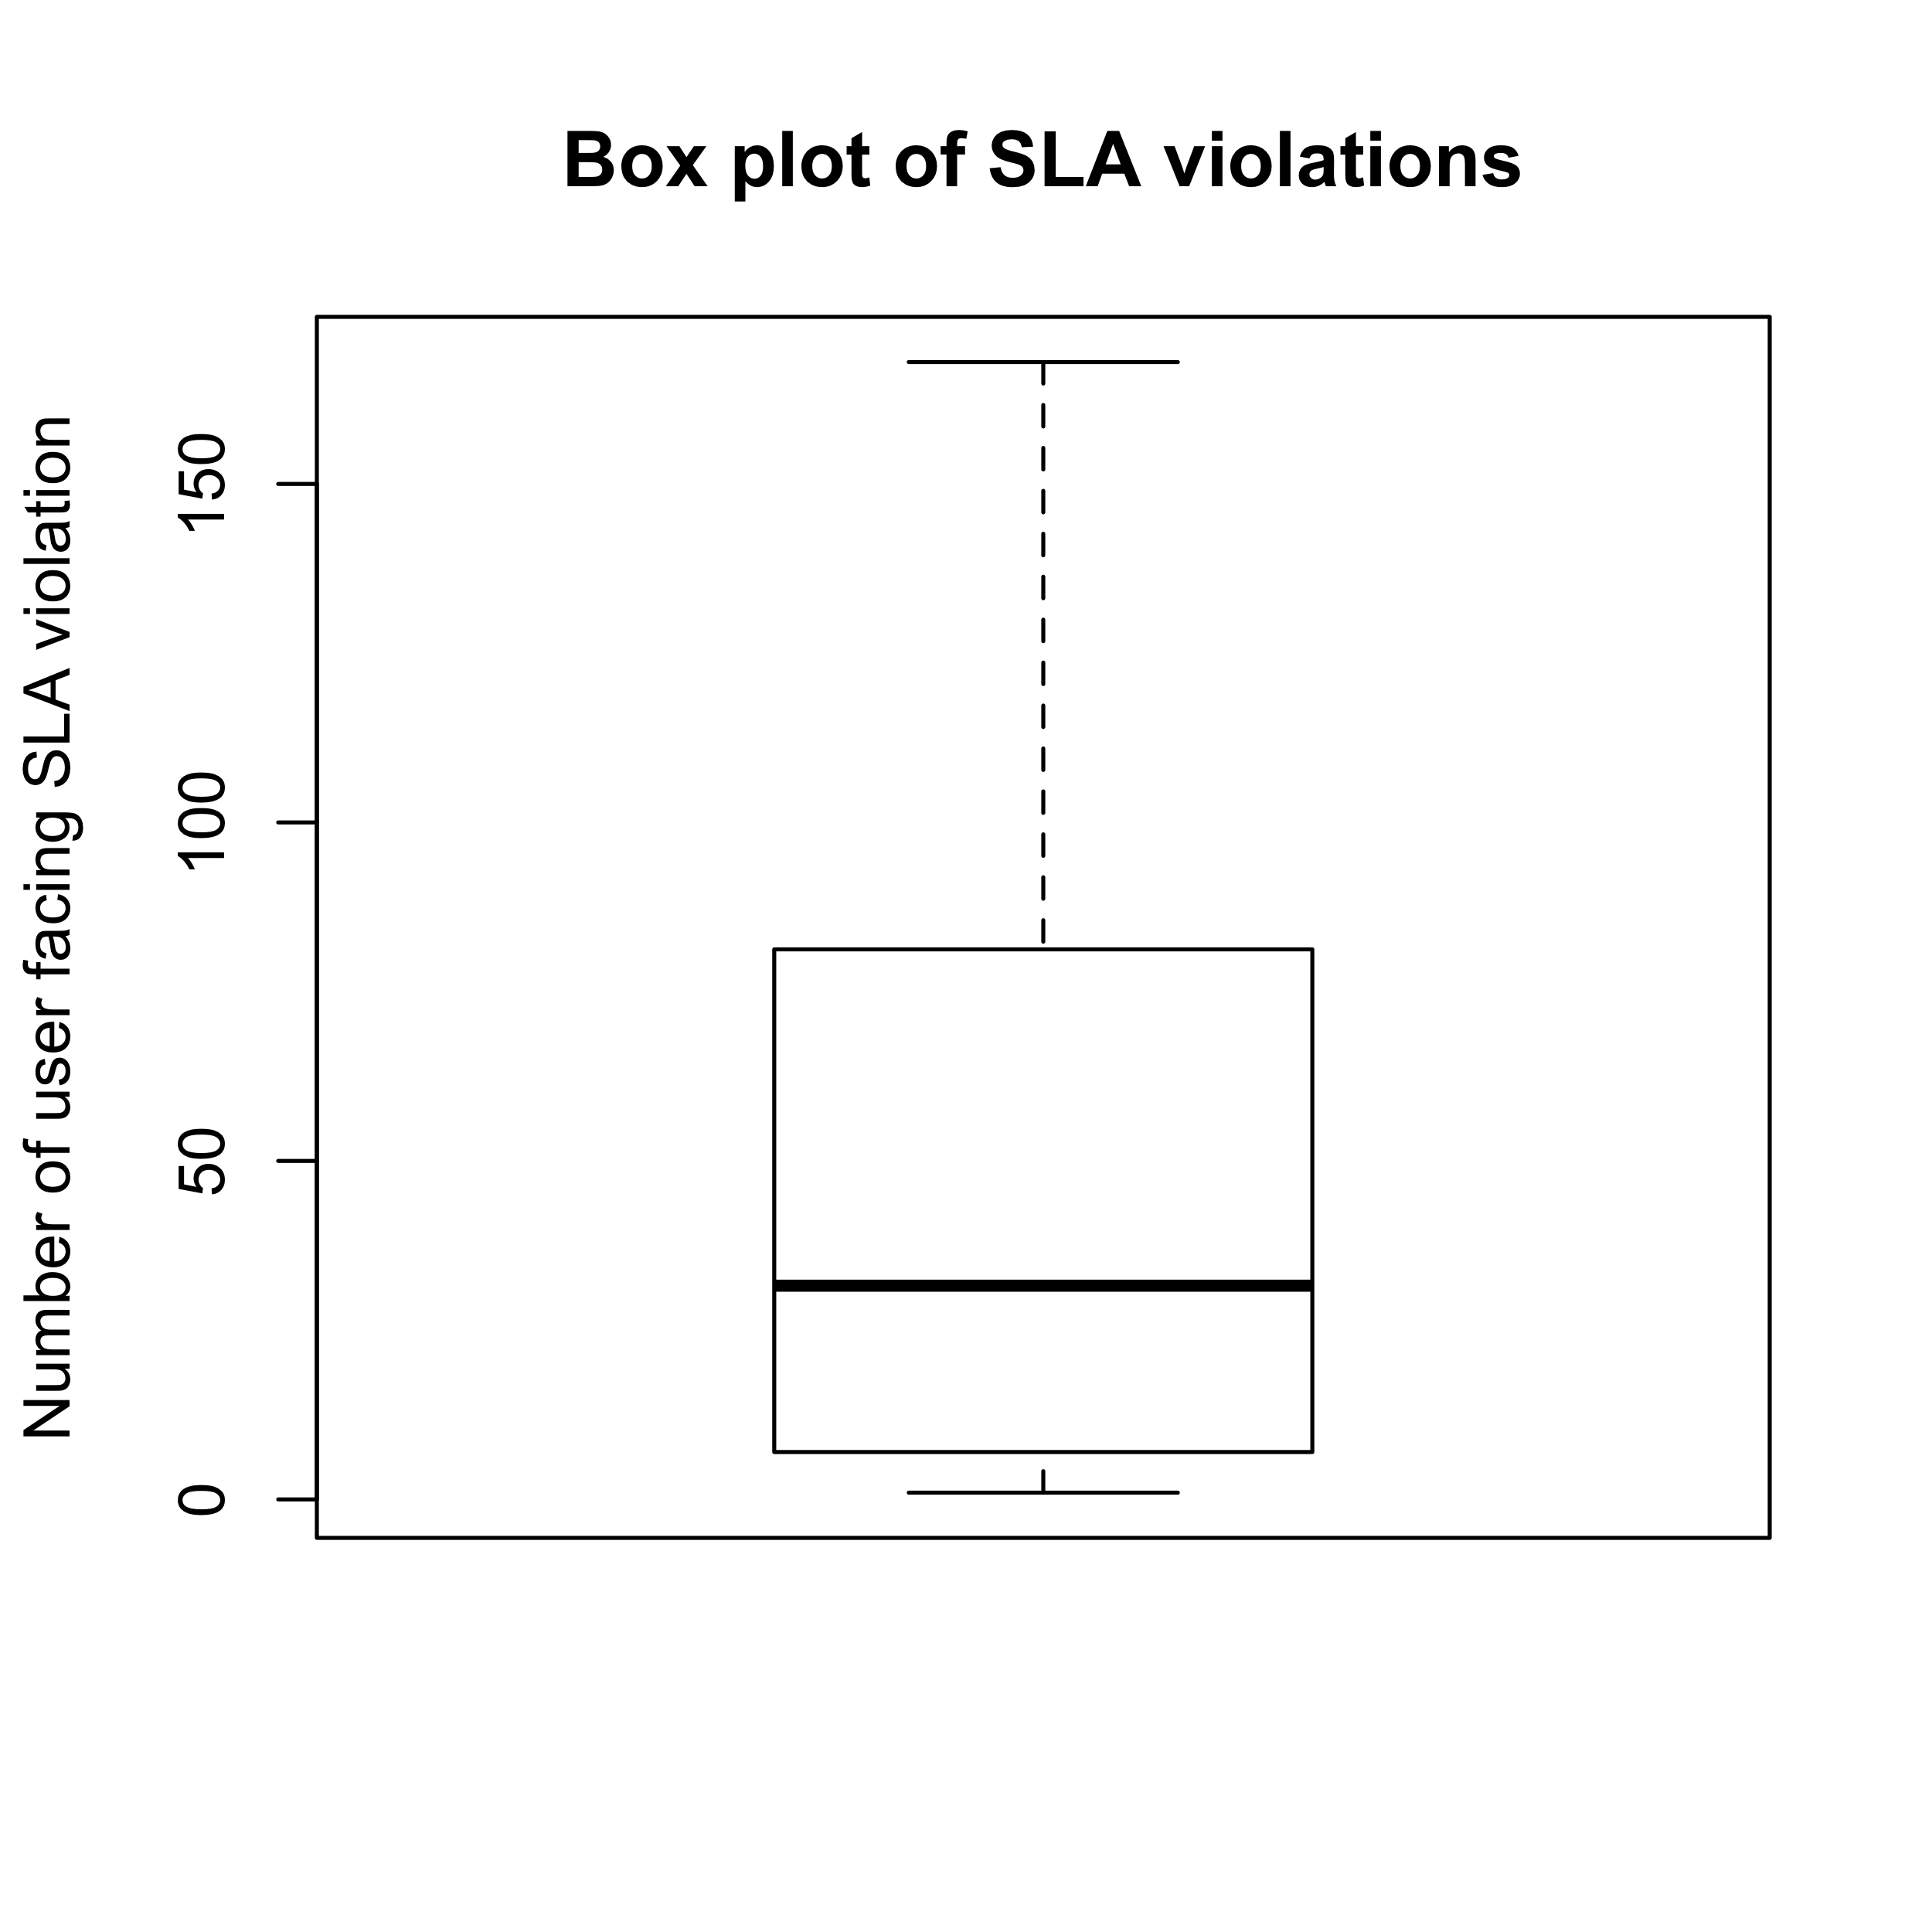
\includegraphics[scale=0.12]{boxplotslaviolation.png}
    \caption{Boxplot of SLA violation}
    \label{figure:boxplotslaviolation}
  \end{center}
\end{figure}
\subsection{Cost Evaluation}
\label{sub:Cost Evaluation}
As discussed in section~\ref{subs:ElasticSim Operation}, ElasticSim given an option of determining how many number of reserved instances to purchase to gain cost benefits\footnote{https://blog.cloudability.com/aws-101-reserved-instances/}. As shown Figure~\ref{figure:purchaseoption}, after running ElasticSim on test workload it produces various option of varying reserved instances. From the Figure~\ref{figure:purchaseoption}, bar graph is grouped into various options. In each option first bar represents the base line price, which is the cost of reserved instances used when serving peak workload. In the scope of this experiment, the base line was calculated for a peak workload of 1070 users. Based on this peak workload, total of 9 VM's are necessary for the period of simulation which is 41 hours and the cost associated with this is USD \$213.2. Since, ElasticSim varies the number of reserve instances to use for providing various option. The second bar represents cost associated with reserving the instances for that particular option. Total number of instances reserved for each option is presented in purple colored bar. Keeping reserved instances fixed through out the simulation, on-demand instances are used for varied workload. The cost associated with on-demand instances are presented in blue bar. The total cost, presented in cyan color, is the sum of reserved instance cost and on-demand instance costs. This total cost is used to make the right instance purchasing choose. Of all the option, option-3 provides a best option for purchasing since the total cost for 3 reserved instance and 18 on-demand instances will cost USD \$158.8. Using purchase option 3, ElasticSim was configured to use total of 3 reserved instances for the simulation duration of 41 hours and the cost benefits of using this option was the saving of USD \$52.45. In figure~\ref{figure:vmlifetime}, y-axis corresponds to VM-ID and x-axis is the time duration of the simulation. Red bars the graphs represents the total time of billing of each VM. Number of minutes used and its associated cost are mentioned next to the plot.
\begin{figure}[h]
  \begin{center}
    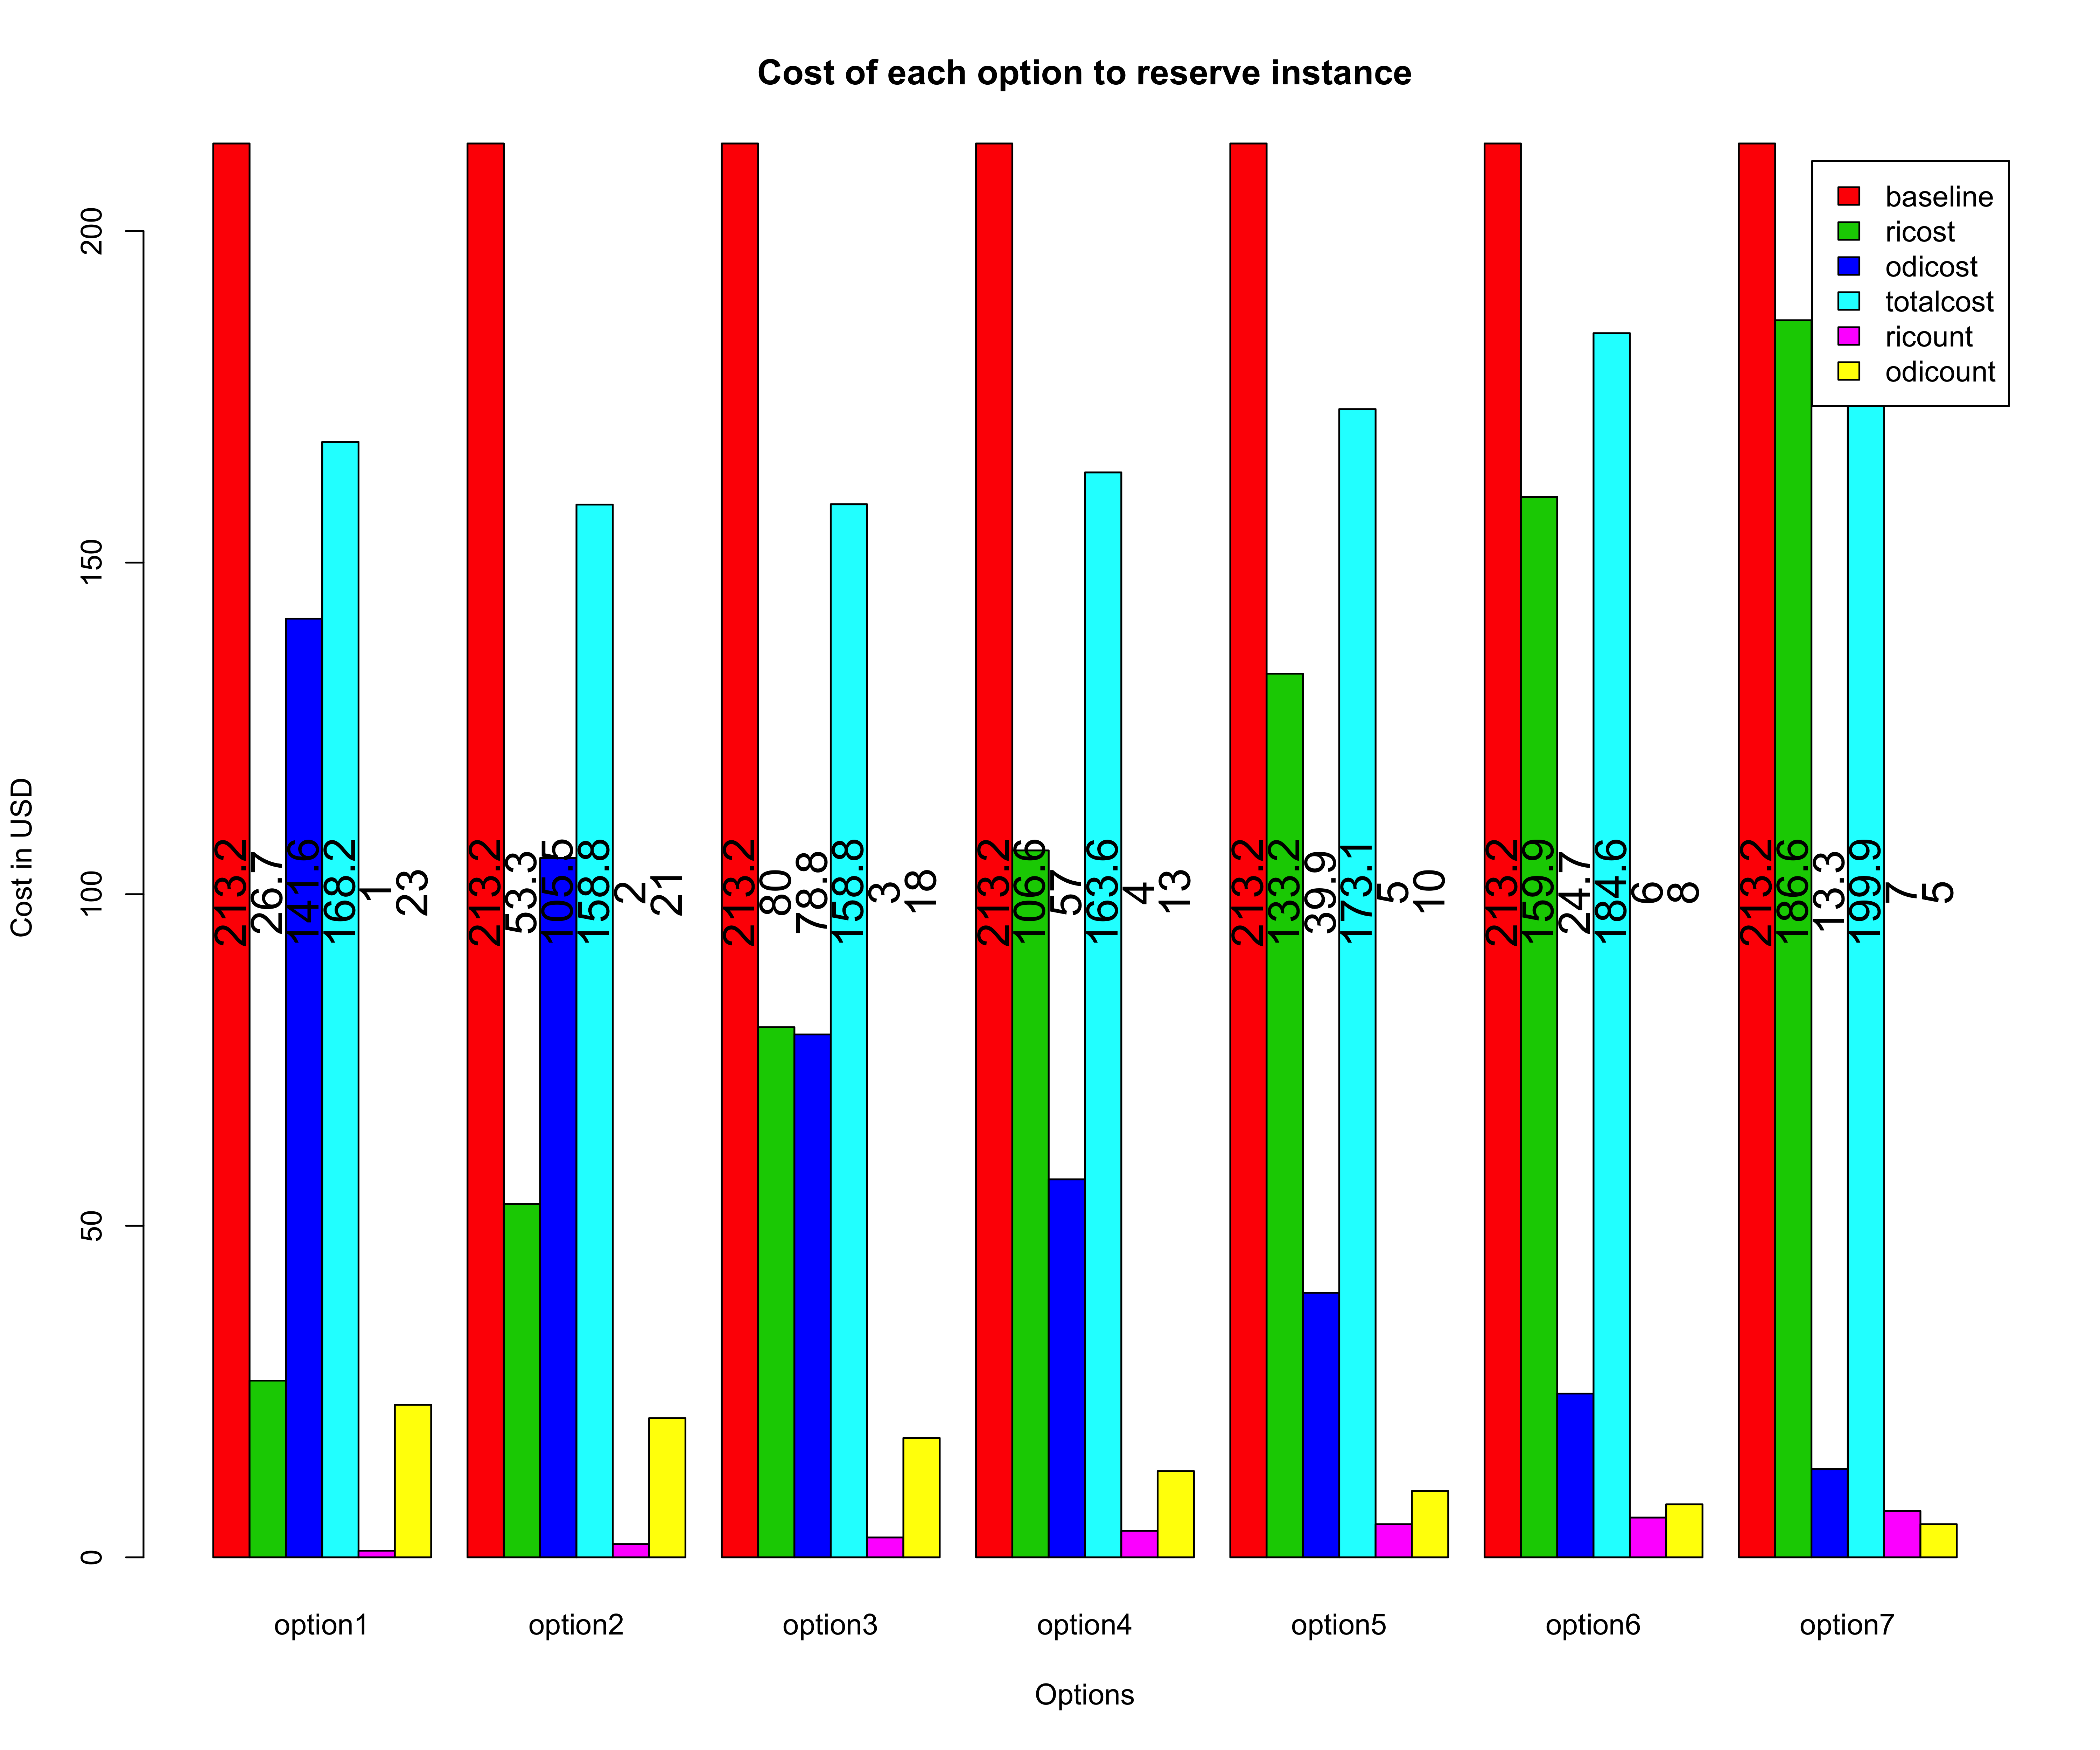
\includegraphics[scale=0.05]{purchaseoption.png}
    \caption{Cost effective instance purchase option}
    \label{figure:purchaseoption}
  \end{center}
\end{figure}


\section{Summary}
\label{sec:Summary}
Section~\ref{section:ElasticSim} provided implementation details of ElasticSim simulator. Implementation details and its internal operations were also presented in this section.
\\
Section~\ref{sec:implementationprediction} implementation details of automated ARIMA forecasting model was presented. Along with forecast model, accuracy measure method called MAPE was explained.
\\
In section~\ref{sec:AppElastic Algorithm Implementation}, implementation details and features of AppElastic algorithm was introduced with few code snippets. Proposed approach is evaluated in the section~\ref{sec:Evaluation} through various facets like: effectiveness of AppElastic algorithm, accuracy of ARIMA model and cost benefits. It showed that, deploying AppElastic with optimal reserved instances can provide significant cost benefits.

\begin{lstlisting}[language=java,caption=AppElastic with RI and ODI instances,label=list:appelasticriodi,numbers=left,frame=single,fontadjust=true,breaklines,basicstyle=\small]
ArrayList<Integer> userInInterval5 = getRequestCountsInTimeRange(timeStamp, timeStamp + timeTakenToActive,false);
Collections.sort(userInInterval5);
int maxUserInterval5 = userInInterval5.get(userInInterval5.size() - 1);
int machineReq = (int) Math.ceil((double)maxUserInterval5 / numberOfUserPerInstance);
// Machines currently being reserved.
int machineRunning = runningRiInstances.size();
// Machines running in ODI
for (int i = 0; i < runningOdiInstances.size(); i++) {
 if(timeStamp <= runningOdiInstances.get(i).endOfActivePeriod)
  machineRunning+=1;
}
if (machineReq > machineRunning) {
 int machinesToAdd = machineReq - machineRunning;
 for (int i = 0; i < machinesToAdd; i++) {
  machineIDWithRI += 1;
  runningOdiInstances.add(new VmInstance(machineIDWithRI, timeStamp, timeStamp + billingPeriod, timeStamp + timeTakenToActive, (timeStamp + billingPeriod) - timetakenToShutdown));
  }
}
ArrayList<Integer> usersInInterval15 = getRequestCountsInTimeRange(timeStamp, timeStamp + scaleDownLookAhead,true);
Collections.sort(usersInInterval15);
int maxUserInterval15 = usersInInterval15.get(usersInInterval15.size() - 1);
int newMachineReq15 = (int) Math.ceil((double)maxUserInterval15 / numberOfUserPerInstance);
ArrayList<VmInstance> vmsEndingActivePeriod = new ArrayList<>();
for (int i = 0; i < runningOdiInstances.size(); i++) {
 if (runningOdiInstances.get(i).endOfActivePeriod == timeStamp) {
  vmsEndingActivePeriod.add(runningOdiInstances.get(i));
  }
}
int totalVmToKill = machineRunning - newMachineReq15;
if (vmsEndingActivePeriod.size() > 0) {
// kill all vm's which are ending active period.
 if ( totalVmToKill >= vmsEndingActivePeriod.size() ) {
  for (int j = 0; j < vmsEndingActivePeriod.size(); j++)
  for (int i = 0; i < runningOdiInstances.size(); i++)
   if (runningOdiInstances.get(i).machineID == vmsEndingActivePeriod.get(j).machineID)
  	runningOdiInstances.get(i).canExtend = false;
}

// kill only subset of vm's ending active period.
if (totalVmToKill < vmsEndingActivePeriod.size()) {
 for (int j = 0; j < totalVmToKill; j++)
 for (int i = 0; i < runningOdiInstances.size(); i++)
  if (runningOdiInstances.get(i).machineID == vmsEndingActivePeriod.get(j).machineID)
   runningOdiInstances.get(i).canExtend = false;
}

for (int i = 0; i < runningOdiInstances.size(); i++) {
 if (timeStamp == runningOdiInstances.get(i).endOfActivePeriod && runningOdiInstances.get(i).canExtend) {
  		runningOdiInstances.get(i).endOfActivePeriod += billingPeriod;
  		runningOdiInstances.get(i).billingHourEndTime += billingPeriod;
 }
}
for (int i = 0; i < runningRiInstances.size(); i++) {
 if (timeStamp == runningRiInstances.get(i).endOfActivePeriod) {
  runningRiInstances.get(i).endOfActivePeriod += billingPeriod;
	runningRiInstances.get(i).billingHourEndTime += billingPeriod;
 }
}
\end{lstlisting}

\begin{figure}[h]
  \begin{center}
    \includegraphics[scale=0.04,angle=90]{vmlifetime.png}
    \caption{Life time of each VM used}
    \label{figure:vmlifetime}
  \end{center}
\end{figure}


\chapter{Discussion and Future Works}
\label{chap:DiscussionOutlook}
This chapter summarizes the achieved goals of this thesis and gives answer to the research questions proposed in Chapter 1. Then a discussion of AppElastic algorithms outlook over possible work can be performed in future.

\section{Achievements}
\label{sec:Achievements}
AppElastic algorithm, as a proactive threshold based horizontal scaling algorithm, provides a customer oriented approach to elasticity for cloud hosted applications. AppElastic algorithm works in collaboration with ARIMA forecast model and relies on models ability to forecast future workloads. It is designed and implemented with ElasticSim simulator based on the principle of easy testability of scaling algorithms and modeling of various components of the cloud.
\\
With the introduction of AppElastic algorithm and ElasticSim following goal where achieved:
\begin{itemize}
  \item Scalability: AppElastic algorithm which was introduced in the section~\ref{subs:AppElastic with Look-ahead}, is the actual scaling agent which horizontally scales the virtual servers to accommodate rapidly changing workloads.
  \item SLA guarantees: The implementation of AppElastic algorithm which was provided in section~\ref{sec:AppElastic Algorithm Implementation} provides SLA aware provisioning of VM's which is an important aspect for the serving consumers.
  \item Cost benefits: ElasticSim simulator which was introduced in the section~\ref{sec:Simulation design} provides various cost saving recommendations based on historical workload analysis. Once the simulator user chooses the best purchasing option. AppElastic algorithm tries to provide best performance scaling action for the given cost.
  \item Testability: ElasticSim simulator implementation provides an easy configurable system. The output generated by the simulator helps in debugging scale algorithm and provide graphic reports for readability purpose.
\end{itemize}

Based on the achievements summarized above as well as the work introduced in the Chapter 4 and Chapter 5, the answers to the research questions proposed in Section~\ref{sec:Research Questions} can be addressed as follows:
\begin{itemize}
  \item What are the parameters to consider while computing the right number of VM resources required to satisfies QoS guarantees?
  \\
  As defined in section~\ref{sec:Classification of elasticity mechanism}, AppElastic is a threshold based automated scaling algorithm. It uses total user request to the application as threshold parameter for compute right number of VM machine resources. As it was showed in section~\ref{sub:Evaluation of AppElastic Algorithm} AppElastic algorithm provide best SLA guarantees, but due it proactive provisioning feature SLA violations will occur.
  \item What are the right VM instance types to use to achieve low operational cost?
  \\
  Based on the heuristics approach employed by ElasticSim. Amazon AWS pricing options as an example, ElasticSim provides its user best possible instance purchase option based on analysis of historical workload trace. Once the historical data is used for instance planning, right number of instance types can be configured to work on actual workload to achieve cost benefits through savings.
  \item What kind of tool and technique can be used to accurately evaluate the performance and cost of the scaling algorithm without actual deployment on the clouds?
  \\
  ElasticSim which was introduced in section~\ref{sec:Simulation design} provides a configurable system to deploy and test any horizontal scaling algorithm. This kind of simulator provides researchers configurable and easy to implement feature.
  \item What are the forecasting techniques which can be used to proactively provision VM's to mitigate effects of delay in VM start and shutdown time?
  \\
  Considering the user request workload as time series data, based on background research ARIMA forecasting techniques which was introduced in ~\ref{sub:ARIMA} was used. As proved in evaluation section~\ref{sub:Forecast Accuracy}, automated ARIMA forecasting model which was used in this thesis provides as small as 1.5\% error in forecasting future workloads.
\end{itemize}
\section{Future Work}
\label{sec:Future Work}
The propose proactive auto scaling method opens up possibility of some new and challenging problems. Some of the possible extensions of the current work are discussed as bellow:
\begin{itemize}
  \item Workload: In this thesis, workload traces from Citrix Audio/Video conferencing application is used as input. Even though it proves to provide cost benefits and SLA guarantees. It has been seen how the AppElastic algorithm performs under test workload and its remain to explore the AppElastic algorithm behavior under production. Other than deploying AppElastic in production, research community has developed various syntactic workload generation tools such as LIMBO\cite{von2014limbo}\footnote{http://descartes.tools/limbo} which can be integrated with AppElastic to model complex workload patterns.
  \item Different forecasting techniques: ARIMA time series forecasting is the only modeling technique applied. Herbst et al.\cite{herbst2012workload} have developed a technique called Workload Classification \& Forecasting (WCF) tool which automatically generates spectrum of forecasting methods based on time series analysis like ARIMA, Extended Exponential Smoothing (ETS), tBATS, etc\cite{herbst2012workload}\footnote{https://github.com/NikolasHerbst/WCF}. Hence integrating AppElastic with such modern tools can be one the future works.
  \item Different threshold parameters: In the current system, number of user request is used as threshold parameter for scaling the system. Performance profiling of an application will provide various other parameters such as CPU load, memory, network utilization, service response time etc. which can be included into AppElastic algorithm as further threshold parameters.
\end{itemize}


\chapter{Conclusion}
\label{chap:Conclusion}

\cleardoublepage
% \phantomsection
\addcontentsline{toc}{chapter}{\listfigurename}
\listoffigures

\cleardoublepage
% \phantomsection
\addcontentsline{toc}{chapter}{List of Algorithms}
\listofalgorithms

\addcontentsline{toc}{chapter}{\listtablename}
\listoftables

\addcontentsline{toc}{chapter}{Bibliography}
\bibliography{handin}

\end{document}
